\documentclass[a4paper,12pt,twoside]{Tesis}

%Packages
\usepackage[nooneline]{subfigure}
\usepackage{url}
\usepackage{afterpage}
\usepackage{amsmath}
\usepackage{amsthm}
\usepackage{amssymb}
\usepackage{amsfonts}
\usepackage{listings}
%\usepackage{theorem}
%\usepackage{thmtools}
\usepackage{alltt}
\usepackage{colortbl}
\usepackage{afterpage}
% \usepackage{a4wide}
\usepackage{setspace}
%\usepackage[T1]{fontenc}
\usepackage{epsfig}
\usepackage{url}
%\usepackage{algorithm}
\usepackage{algorithmicx}
\usepackage{algpseudocode}
\usepackage{color}
%\usepackage{setspace}
\usepackage{textcomp}
\usepackage{mathcomp}
\usepackage{fontenc}
\usepackage{float}
%\usepackage[hyperindex,bookmarks,ps2pdf,dvips,breaklinks=true,linktocpage]{hyperref}
\usepackage[hyperindex,bookmarks,dvipdfm,dvips,breaklinks=true,linktocpage]{hyperref}
\usepackage{breakurl}
\usepackage{algorithm}
%\usepackage{algorithmic}
%\usepackage{metre}
%\usepackage{yhmath}
\usepackage{textcomp}
\usepackage{tabulary}
\usepackage{multicol}
\usepackage{caption}
%\usepackage{subcaption}
\usepackage{url}
\usepackage{graphicx}
\usepackage{caption}
\usepackage{subcaption}


\newtheoremstyle{example}{\topsep}{\topsep}%
     {}%         Body font
     {}%         Indent amount (empty = no indent, \parindent = para indent)
     {\bfseries}% Thm head font
     {}%        Punctuation after thm head
     {\newline}%     Space after thm head (\newline = linebreak)
     {\thmname{#1}\thmnumber{ #2}\thmnote{ #3}}%         Thm head spec

   \theoremstyle{example}
   \newtheorem{example}{Example}[section]

%%%Mathematical definitions%%%
\newcommand{\pclock}{\cal{P}}

\newtheorem{definition}{Definition}%[chapter]
%\newcommand{\bdfn}{\begin{definition} \begin{rm}}
%\newcommand{\edfn}{\vspace{-2ex}
%{\flushright $\Box$\\
%\mbox{}\vspace{-2ex}
%} \end{rm} \end{definition}}
%\newcommand{\edfnt}{ \end{rm} \end{definition}}
%
%\newcommand{\bthm}{\begin{theorem} \begin{rm}}
%\newcommand{\ethm}{\vspace{-4ex}{\flushright $\Box$\\
%\mbox{}\vspace{-4ex}} \end{rm} \end{theorem}}
%\newcommand{\bprop}{\begin{proposition} \begin{rm}}
%\newcommand{\eprop}{\vspace{-4ex}{\flushright $\Box$\\
%\mbox{}\vspace{-4ex}} \end{rm} \end{proposition}}
%\newcommand{\bcor}{\begin{corollary}\begin{rm}}
%\newcommand{\ecor}{\vspace{-4ex}{\flushright $\Box$\\
%\mbox{}\vspace{-4ex}} \end{rm} \end{corollary}}
%\newcommand{\blem}{\begin{lemma} \begin{rm}}
%\newcommand{\elem}{\vspace{-4ex}{\flushright $\Box$\\
%\mbox{}\vspace{-4ex}} \end{rm} \end{lemma}}
%\newcommand{\bfact}{\begin{fact} \begin{rm}}
%\newcommand{\efact}{\vspace{-4ex}{\flushright $\Box$\\
%\mbox{}\vspace{-4ex}} \end{rm} \end{fact}}
%\newcommand{\bex}{\begin{example} \begin{rm}}
%\newcommand{\eex}{\vspace{-2ex}{\flushright $\Box$\\
%\mbox{}\vspace{-2ex}} \end{rm} \end{example}}
%\newcommand{\narrow}{$\!${\scriptsize N}$\! \longrightarrow$}
%\newcommand{\narrowast}{$\!${\scriptsize N}$\!
% \stackrel{\ast}{\longrightarrow}$}
%\newcommand{\narrowur}{$\!${\scriptsize N}$\!
% \stackrel{<u,r>}{\longrightarrow}$}
\newcommand{\impast}{\stackrel{\ast}{\Longrightarrow}}
\newcommand{\entero}{\mathbb{Z}}
\newcommand{\bs}{[\![}
\newcommand{\es}{]\!]}
%\newcommand{\nat}{{\nnul}
%\newcommand{\eneg}{\hspace*{-0.15cm}}
%\newcommand{\real}{\rm I\! R}
%\newcommand{\barra}{\, | \,}
%\newcommand{\nbar}{\, \mid \hspace*{-1.25ex} \sim \,}
\newcommand{\prim}[1]{{\it Ft( #1 )}}
\newcommand{\interle}{|\hspace*{-0.04cm}\|}
\long\def\comment#1{}
\newcommand{\regla}[3]{\renewcommand{\arraystretch}{0.75}
\begin{array}{c}
\displaystyle #1\\
\rule{#3cm}{0.1mm}\\
\displaystyle #2
\end{array}\renewcommand{\arraystretch}{1.0}
}
\newcommand{\reglaa}[3]{\renewcommand{\arraystretch}{0.5}
\begin{array}{c}
\displaystyle #1\\
\rule{#3cm}{0.1mm}\\
\displaystyle #2
\end{array}\renewcommand{\arraystretch}{1.0}
}
\newcommand{\separ}{\vspace*{0.1cm}}
\newcommand{\reglal}[1]{
\frac{\;\;#1}{\;~~~~~\;}\!\!\!\!\rightarrow}
\newcommand{\reglasl}[1]{
\frac{\;\;\scriptstyle #1}{\;~~~~~~~~~~~~~~\;}\!\!\!\rightarrow}
\newcommand{\Regla}[1]{\stackrel{#1}{\Longrightarrow}}
\newcommand{\reglad}[2]{\renewcommand{\arraystretch}{0.5}
\begin{array}[t]{c}
\rule{#2cm}{0.1mm}\\
\displaystyle #1
\end{array}\renewcommand{\arraystretch}{1.0}}
\newcommand{\maximo}[1]{\renewcommand{\arraystretch}{0.40}
\begin{array}[t]{c}
{\it Max}\\
{\scriptstyle #1}
\end{array}\renewcommand{\arraystretch}{1.0}}
\newcommand{\minimo}[1]{\renewcommand{\arraystretch}{0.40}
\begin{array}[t]{c}
{\it Min}\\
{\scriptstyle #1}
\end{array}\renewcommand{\arraystretch}{1.0}}
\newcommand{\To}{\longrightarrow}
\newcommand{\flecha}[1]{\stackrel{#1}{\longrightarrow}}
\newcommand{\flechad}[2]{
\renewcommand{\arraystretch}{0.5}
\begin{array}{c}
{\scriptstyle #1}\\
\rightarrow\\
{\scriptstyle #2}\\
\end{array}
\renewcommand{\arraystretch}{1}
}
\newcommand{\flechal}[1]{\stackrel{#1}{-\!\!-\!\!\!\longrightarrow}}
\newcommand{\flechald}[2]{\renewcommand{\arraystretch}{0.5}
\begin{array}{c}
{\scriptstyle #1}\\
\longrightarrow\vspace*{-0.1cm}\\
{\scriptstyle #2}
\end{array}
\renewcommand{\arraystretch}{1}
}
\newcommand{\flechalu}[2]{\renewcommand{\arraystretch}{0.5}
\begin{array}{c}
{\scriptstyle #1}\\
\longrightarrow_u\vspace*{-0.1cm}\\
{\scriptstyle #2}
\end{array}
\renewcommand{\arraystretch}{1}
}
\newcommand{\menos}{\renewcommand{\arraystretch}{0.0002}
\begin{array}[b]{c}
\mbox{\small{.}} \\
-
\end{array}\renewcommand{\arraystretch}{1.0}}
\newcommand{\precond}[1]{\hspace*{-0.4em}~^{\bullet}
\hspace*{-0.05em}#1}
\newcommand{\nofalla}{
\stackrel{{\it fail}}{\longrightarrow}
\hspace*{-0.35cm}/
}
\newcommand{\nofallaa}{
\stackrel{{\it fail}}{\longrightarrow}
\hspace*{-0.45cm}/
}
\newcommand{\pila}[2]{\renewcommand{\arraystretch}{0.18}
\begin{array}[t]{c}
#1\\
{\scriptstyle #2}
\end{array}\renewcommand{\arraystretch}{1.0}}
\newcommand{\reglat}[1]{\pila{\longmapsto}{#1}}
\newcommand{\Computacion}[1]{\renewcommand{\arraystretch}{0.60}
\begin{array}[b]{c}
{\scriptstyle #1}\\
\Longrightarrow
\end{array}
\renewcommand{\arraystretch}{1.0}
}
\newcommand{\comentario}[1]{}
\newcommand{\andabajo}[1]{\renewcommand{\arraystretch}{0.40}
\begin{array}[t]{c}
{\Large \wedge}\\
{\scriptstyle #1}
\end{array}\renewcommand{\arraystretch}{1.0}}
\newcommand{\sumas}[1]{\renewcommand{\arraystretch}{0.42}
\hspace*{-0.1cm}
\begin{array}[t]{c}
{\mbox{\Large $\Sigma$}}\\
{\scriptstyle #1}
\end{array}\hspace*{-0.1cm}\renewcommand{\arraystretch}{1.0}}

%suma con cosas arriba y debajo
\newcommand{\suma}[2]{\renewcommand{\arraystretch}{0.42}
\hspace*{-0.1cm}
\begin{array}{c}
{\scriptstyle #2}\\
{\mbox{\Large $\Sigma$}}\\
{\scriptstyle #1}
\end{array}\hspace*{-0.1cm}\renewcommand{\arraystretch}{1.0}}

%Settings
\clubpenalty=10000
\widowpenalty=10000
\newtheorem{theorem}{Theorem}[section]
\newtheorem{lemma}{Lemma}[section]
\newtheorem{remark}{Remark}[section]
%tapn
%new macros
\newcommand{\Turg}{\ensuremath{T_{\mathit{urg}}}}
\newcommand{\sqrel}[2]{\ensuremath{{#1}\sqsubseteq{#2}}}
\newcommand{\cutsqrel}[2]{\ensuremath{{#1}\sqsubseteq_{cut}{#2}}}
\newcommand{\reachmark}[1]{\ensuremath{[#1\rangle}} % [M>
\newcommand{\itn}[1]{\ensuremath{{\mathit{#1}}}}
\newcommand{\jindex}{\ensuremath{{\mathit{\{1,\ldots,m\}}}}}
\newcommand{\iindex}{\ensuremath{{\mathit{\{0,\ldots,n\}}}}}
\newcommand{\consumei}{\ensuremath{{\mathit{Consume_i}}}}
\newcommand{\consumeij}[1]{\ensuremath{{\mathit{Consume_{#1}}}}}
\newcommand{\producei}{\ensuremath{{\mathit{Produce_i}}}}
\newcommand{\produceij}[1]{\ensuremath{{\mathit{Produce_{#1}}}}}
\newcommand{\tai}{\ensuremath{{\mathit{T_{y,i}}}}}
\newcommand{\taif}{\ensuremath{{\mathit{T^{\mathit{flag}}_{y,i}}}}}
\newcommand{\taip}{\ensuremath{{\mathit{T^{\mathit{place}}_{y,i}}}}}
\newcommand{\taj}[2]{\ensuremath{{\mathit{T_{#1,#2}}}}}
\newcommand{\tajp}[2]{\ensuremath{{\mathit{T^{\mathit{place}}_{#1,#2}}}}}
\newcommand{\tajf}[2]{\ensuremath{{\mathit{T^{\mathit{flag}}_{#1,#2}}}}}
\newcommand{\agexi}[2]{\ensuremath{{\mathit{age({#1,#2})}}}}
\newcommand{\fr}[1]{\ensuremath{{\mathit{fract(#1)}}}}
\newcommand{\inte}[1]{\ensuremath{{\mathit{int(#1)}}}}
\newcommand{\rankeq}{\ensuremath{{\mathit{\cong}}}}
\newcommand{\notrankeq}{\ensuremath{{\mathit{\ncong}}}}
\newcommand{\multiset}[1]{\ensuremath{\mathit{\{\!\!\{#1\}\!\!\}}}}
\newcommand{\alist}[1]{\ensuremath{\mathit{<\!\!#1\!\!>}}}
\newcommand{\rank}[2]{\ensuremath{{\mathit{rank_{#1}(#2)}}}}
\newcommand{\tokens}{\mathcal{T}}
\newcommand{\abstmarking}{\mathbb{M}}
\newcommand{\abstinn}{\mathscr{In}}
\newcommand{\abstout}{\mathscr{Out}}
\newcommand{\abstmarkingsof}[1]{\ensuremath{\mathscr{A}(#1)}}
\newcommand{\abstoken}{\ensuremath{{\mathit{(r,p,\ell,c)}}}}
\newcommand{\absmarktriple}[1]{\ensuremath{{\mathit{#1}}}}
\newcommand{\cupdiamond}{\mathbin{\mathaccent\diamond\cup}} % Added by Jose to denote the merge
\newcommand{\cupdot}{\mathbin{\mathaccent\cdot\cup}} % Added by Jose to denote the disjoint operator
\newcommand{\fire}{\ensuremath{{\mathit{fire((p,t))}}}}
\newcommand{\enable}{\ensuremath{{\mathit{enable((p,t))}}}}
\newcommand{\rankM}[1]{\ensuremath{{\mathit{rank(#1)}}}}
\newcommand{\fireM}{\ensuremath{{\mathscr{F}}}}
\newcommand{\transM}{\ensuremath{{\mathscr{Trans}}}}

\newcommand{\initstack}{\ensuremath{\mathit{InitStack()}}}
\newcommand{\noinf}{\ensuremath{\mathit{maxBound}}}
\newcommand{\sizeofmarking}{\ensuremath{\mathit{size}}}
\newcommand{\tapntuple}{\ensuremath{(P, T, \Turg, \ia,\allowbreak \oa, \cfunction, \wfunction, \type, \inv)}}
%\newcommand{\tawfntuple}{\ensuremath{(P_w \cup P_r, T, \ia,\allowbreak \oa, \cfunction, \wfunction)}} % Added by Jose to model Timed-Arc workflow nets
\newcommand{\rctawfntuple}{\ensuremath{(P, T, \ia,\allowbreak \oa, in, out, \cfunction, \wfunction, \type, \inv)}} % Added by Jose to model Resource Constrained Timed-Arc workflow nets
%\newcommand{\productiontuple}{\ensuremath{(P_p , T, \ia_p ,\allowbreak \oa_p , \cfunction, \wfunction)}} % Added by Jose to model the production net of Resource Constrained Timed-Arc workflow nets
\renewcommand{\int}{\ensuremath{\mathcal{I}}}
\newcommand{\intinv}{\int^{\text{inv}}}
\newcommand{\outup}[1]{\mathit{Out}^{#1}}
\newcommand{\inup}[1]{\mathit{In}^{#1}}
\newcommand{\proc}{\ensuremath{\mathit{S}}}
%\newcommand{\lab}{\ensuremath{\mathit{Act}}}
%\newcommand{\act}{\ensuremath{\mathit{Labels}}}
\newcommand{\act}{\ensuremath{\mathit{Act}}}
\newcommand{\queryset}{\mathcal{Q}}
\newcommand{\querytype}{QUERYTYPE}
\newcommand{\places}{\mathit{Places}}
\newcommand{\false}{\mathit{ff}}
\newcommand{\true}{\mathit{tt}}
\newcommand{\ef}{\mathit{EF}}
\newcommand{\cut}{\mathit{cut}}
\newcommand{\caufunc}{\mathit{cau}}
\newcommand{\typefour}{\mathit{IV}}
\newcommand{\typeone}{\ensuremath{\mathit{Inv}}}
\newcommand{\typetwo}{\ensuremath{\mathit{Dead}}}
\newcommand{\typethree}{\ensuremath{\mathit{Std}}}
\newcommand{\cat}{\ensuremath{\mathit{cat}}}
\newcommand{\ia}{\ensuremath{\mathit{IA}}}
\newcommand{\oa}{\ensuremath{\mathit{OA}}}
\newcommand{\cfunction}{\ensuremath{\mathit{g}}}
\newcommand{\wfunction}{\ensuremath{\mathit{w}}}
\newcommand{\type}{\ensuremath{\mathit{Type}}}
\newcommand{\smalltype}{\ensuremath{\mathit{type}}}
\newcommand{\inv}{\ensuremath{\mathit{I}}}
\newcommand{\types}{\mathbf{{Types}}}
\newcommand{\inn}{\ensuremath{\mathit{In}}}
\newcommand{\out}{\ensuremath{\mathit{Out}}}
\newcommand{\inhib}{\mathit{Inhib}}
\newcommand{\transporti}{\ensuremath{\mathit{Transport}_j}}
\newcommand{\transportone}{\ensuremath{\mathit{Transport}_1}}
\newcommand{\transport}{\mathit{Trans}}
\newcommand{\eqMarking}{\equiv}
\newcommand{\gMarking}{>}
\newcommand{\lMarking}{<} 
\newcommand{\enablfunc}{\hat{T}_N}
\newcommand{\nnul}{\mathbb{N}_{0}}
\newcommand{\rnul}{\mathbb{R}^{\geq 0}}
\newcommand{\nuptok}[1]{\mathbb{N}_{0}^{#1}}
\newcommand{\markingsof}{\mathcal{M}}
%\newcommand{\path}[2]{#1 \Rightarrow^* #2}
\newcommand{\qquestion}[3]{\framebox{ \minibox{{\bf Problem:}\ #1 \\ {\bf Instance:} #2 \\ {\bf Question: #3}}}}% Added by Jose to make question environment
\newcommand{\trans}[1]{\stackrel{#1}{\rightarrow}}
\newcommand{\transbdss}[1]{\stackrel{#1}{\rightarrow}_{\textrm{BDS}}}
\newcommand{\transbds}{\rightarrow_{\textrm{BDS}}}
\newcommand{\notrans}{\ensuremath{\nrightarrow}}
\newcommand{\eqdef}{\stackrel{\textrm{def}}{=}}
\newcommand{\powerset}{\mathcal{P}}
\newcommand{\rbigeq}{\mathbb{R}_{\geq 0}}
\newcommand{\cutmold}{\cut(M)_{>}}
\newcommand{\cutyoung}{\cut(M)_{\leq}}
\newcommand{\mold}{M_{>}}
\newcommand{\myoung}{M_{\leq}}
\newcommand{\moldone}{{M_{1}}_{>}}
\newcommand{\moldtwo}{{M_{2}}_{>}}
\newcommand{\real}{\mathbb{R}}
\newcommand{\nbig}{\mathbb{N}}
\newcommand{\causality}{\ensuremath{\mathit{Causality}}}
\newcommand{\mc}{\ensuremath{\mathit{MC}}}
\newcommand{\mcarc}{\ensuremath{\mathit{C}_{arc}}}
\newcommand{\nextInv}{\ensuremath{\mathit{NextInv}}}
\newcommand{\mcplace}{\ensuremath{\mathit{C}_{place}}}
\newcommand{\cmax}{\ensuremath{\mathit{C}_{max}}}
\newcommand{\normal}{\ensuremath{\mathit{Normal}}}
\newcommand{\waiting}{\ensuremath{\mathit{Waiting}}}
\newcommand{\passed}{\ensuremath{\mathit{Passed}}}
\newcommand{\trace}{\ensuremath{\mathit{Trace}}}
\newcommand{\addpw}{\ensuremath{\mathit{AddToPW}}}
\newcommand{\eq}{\ensuremath{_{\mathit{eq}}}}
%\renewcommand{\top}{\ensuremath{\mathit{top}()}}
\newcommand{\pop}{\ensuremath{\mathit{pop}()}}
%\newcommand{\note}[1]{{\color{red} NOTE: #1}}
\newcommand{\ceq}{:=}
\newcommand{\push}{\ensuremath{\mathit{push}}}
\newcommand{\emptystack}{\ensuremath{\mathit{isEmpty}()}}
\newcommand{\validSuc}{\ensuremath{\mathit{validSuccessors}}}
\newcommand{\successor}{\ensuremath{\mathit{successors}}}
\newcommand{\maxrunend}{\ensuremath{\mathit{endOfMaxRun}}}
\newcommand{\cpp}{C{}\texttt{++}}
\newcommand{\inmark}{\ensuremath{\mathit{M_{in}}}}
\newcommand{\outmark}{\ensuremath{\mathit{M_{out}}}}
%\newcommand{\question}{\framebox{}}



%%%%%%%%%%%%%%%%%%%%%%%%%%%%%%%%%%%%%%%%%%%%%%%%%%%%%%%%%%%%%%%%%%%%%%%%%%%%%%%%%%%%%%%%%%%%%%
\begin{document}

\autor{Jos\'e Antonio Mateo Cort\'es}
\titulo{Verification and Validation of Web Service Compositions using Formal Methods}
\fecha{}
\tutorA{Dr.~Valent\'in Valero Ruiz}
\tutorB{Dr.~Ji\v{r}\'{\i} Srba}

\maketitle

\frontmatter

\setstretch {1.5}

\section*{Acknowledgements}

To be added.

\chapter*{Abstract}\label{c0}

Nowadays, most of the computing systems are based on service-oriented computing (SOC). 
This paradigm aims at replacing complex monolithic systems by a composition of interacting systems
called services. A service encapsulates self-contained functionality and offers it over
a well-defined and standardized interface. It allows cross-organizational collaborations 
in which each participant is in charge of a particular tasks leading to 
the development of scalable, flexible and low-cost distributed applications. Each service
works as an autonomous component, performing only the tasks for which it has been implemented. 
As the development of such services is independent, companies can reuse a considerable amount of components, 
thus saving money and time. Moreover, these technologies are widely used 
due to their ability to provide interoperability among services 
from different companies since all the participants know the services offered by the others as well as how to access them. 

Due to privacy concerns or commercial policy, entities participating in one of 
these architectures have no access to complete information, that is, 
he code implementing the services the particpants consume is hidden, 
thus being impossible to examine or verify the implementation of the consumed services.
Another issue is that web services are usually \emph{stateless},
which means that no state is stored from the clients viewpoint. 
However, some new applications and services have emerged, which
require to capture the state of some resources. Thus,
new standards to manage the state of a web service have appeared. For instance,
Open Grid Services Infrastructure (OGSI) was conceived to allow designers to manage resources when using web services, and
this standard became Web Services Resource Framework (WSRF) when new improvements were introduced. 

Obviously, in this scenario the probability of making errors is higher than working in a monolithic scenario. Therefore, there is
a clear need of applying any kind of technique to ensure the correctness of each participant and their composition.
In this Thesis, we present a formal language called BPELRF and its semantics. The aim of this language is
to model a set of bussiness processess implemented in the de-facto standard modelling language, WS-BPEL, but
enriched with the ability to manage distributed resources. These distributed resources are managed according to
the guidelines provided by the standard WSRF. Moreover, we provide a visual model of this language in terms of 
coloured Petri nets in order to ease uninitiated people to deal with it, and we use the well-known toolbox, CPNTools,
to verify the composition of web services with distributed resources expressed in BPELRF. As usual, the process of building manually
the Petri nets model of large scenarios is time-consuming and error-prone. Therefore,
we have implemented a tool to support web designers that, given a BPELRF specification, it extracts automatically the coloured 
Petri nets of the scenario. Finally, this model can be verified using CPNTools.

On the second part of the Thesis, we extend the classical definition of Workflow nets with time features. 
Workflow nets were introduced 
by Wil van der Aalst as a formalism
for the modelling, analysis and verification of business workflow processes.
%to model, validate and verify business process, \emph{workflow nets} (wf-nets) \cite{Aalst97,Aalst98}. 
The formalism is based on Petri nets abstracting away most of the data 
while focusing on the possible flow in the system. 
Its intended use is in finding design errors 
such as the presence of deadlocks, livelocks 
and other anomalies in workflow processes. Such correctness criteria can
be described via the notion of \emph{soundness} that
requires the option to complete the workflow, guarantees proper termination
and optionally also the absence of redundant tasks. 

After the seminal work on workflow nets, researchers have 
invested much effort in defining new soundness criteria and/or 
improving the expressive power of the original model by adding new features 
and studying the related decidability and 
complexity questions.
%such as reset or inhibitor arcs, resources, time or multiple instances. 
%It is impossible and is also out of the scope of this paper to summarise here all
%of these works, and, therefore, we refer the interested reader to \cite{AalstHHSVVW11} for further information. 
%Nevertheless, it is worthwhile to
%mention that there is a common characteristic in all of this extended models: undecidability. Thus, soundness (or its different variants)
%is decidable for classical workflow nets \cite{Aalst97}, but, for instance, it is undecidable when we add reset or inhibitor arcs \cite{AalstHHSVVW11}.
In this Thesis, we define a quantitative extension of workflow 
nets with timing features called timed-arc Workflow nets. It allows us to argue, among others, 
about the execution intervals of tasks, deadlines and urgent behaviour of workflow processes. Our workflow
model is based on timed-arc Petri nets
where tokens carry timing information
and arcs are labelled with time intervals restricting the available
ages of tokens used for transition firing. Here, we consider both discrete and continuous time
semantics, thus conforming a whole theory of workflow nets. Finally, all the theory presented in 
this thesis have been introduced in the tool Tapaal, offering researchers a mean to model 
timed-arc workflow nets and to automatically verify (strong) soundness.



\tableofcontents
\cleardoublepage

\listoffigures
\cleardoublepage

\listoftables
\cleardoublepage

%\listofalgorithms
%\cleardoublepage

\parskip=6pt


%%%%%%%%%%%%%%%%%%%%%%%%%%%%%%%%%%%%%%%%%%%%%%%%%%%%%%%%%%%%%%%%%%%%%%%%%%%%%%%%%%%%%%%%%%%%%%
\mainmatter

\pagestyle{headings}

\chapter{Introduction}\label{chapter:c1}
\markboth{Chapter~\ref{chapter:c1}. Introduction}{}

\section{Motivation}\label{scope}
\markright{~\ref{scope}Motivation}

The development of software systems is becoming more complex with the 
appearance
of new computational paradigms such as Service-Oriented  Computing  (SOC), 
Grid Computing and Cloud Computing.
In these systems, the service provider needs to ensure some levels of 
quality and privacy to the final
user in a way that had never been raised. It is therefore necessary 
to develop new techniques to benefit from the advantages 
of recent approaches, as Web service compositions. 
Formal models of concurrency have been widely used for the description and analysis of concurrent and distributed systems. 
Grid/Cloud environments are characterized by a dynamic environment 
due to the heterogeneity and volatility of resources. 
There are two complementary views in composite web services: Choreography and Orchestration. 
The choreography view describes the observable interactions among services and can
be  defined  by  using  specific  languages such as Web  Services
Choreography  Description  Language  (WS-CDL), %\cite{WSCDL}
or  by
using some more general languages like UML Messages Sequence
Charts (MSC). On the other hand, orchestration concerns
the internal behaviour of a Web service in terms of invocations
to  other  services.  Web Services Business 
Process Execution Language (WS-BPEL) \cite{Andrews2003WSBPEL} is normally used 
to describe Web service orchestrations, so this
is considered the de-facto standard language for describing Web services
workflows in terms of web service compositions. 

To facilitate additional interoperability among services, more standardization is required to deal with distributed resources. In January of 2004, several members of the \emph{Globus Alliance} organization and the computer multinational \emph{IBM} with the help of experts from companies such as \emph{HP, SAP, Akamai, etc.} defined the basis architecture and the initial specification documents of a new standard for that purpose, Web Services Resource Framework (WSRF)~\cite{Ban06,WSRFstandard}. Although the Web service 
definition does not consider the notion of state, interfaces frequently provide the user with the ability to access and manipulate
states, that is, data values that persist across, and evolve as a result of Web service interactions. The messages that the services 
send and receive imply (or encourage programmers to infer) the existence of an associated stateful resource. It is then desirable 
to define Web service conventions to enable the discovery of, introspection on, and interaction with stateful resources in standard 
and interoperable ways~\cite{foster2004}. 

The main motivation of the first part of the Thesis is to provide a formal 
semantics for WS-BPEL+WSRF to manage stateful Web services workflows 
by using the existing machinery in distributed systems,
and specifically a well-known formalism, such as prioritised-timed
coloured Petri nets, which are not only a graphical model, but they also
provide us with an easier way to simulate and analyse the modelled
system. Thus, our aim is not to provide just another WS-BPEL semantics. 
In order to deal with the integration of BPEL plus WSRF in a proper way, 
we have realized that it is more convenient 
to introduce a specific semantic model, which  covers 
properly all the relevant aspects of WSRF such as notifications and 
resource time-outs. 
The integration of WS-BPEL and WSRF is not new; in the literature, 
there are a bundle of works defining this integration, but 
none of these works define a formal semantics in terms of Petri
nets.

The aim of the second part of the Thesis is to extend a mature formalism like
Workflow nets with time features. To this end, we use timed-arc Petri nets, where
each token has attached a timestamp, allowing to measure, for instance, execution times. 
Workflow nets are useful when designing how the participants of a business process interact
and in which order. Thus, it is easy to check bottlenecks or undesirable behaviour in our processes.
Moreover, we prove the decidability (or undecidability) of a fundamental property for workflow nets, soundness.
This property is checked using a continuous and a discrete time semantics. To add value to our workflow theory, we have included
it into a well-known tool, Tapaal.
 
\section{Objectives}\label{objectives}

Next, we describe the general and specific objectives of the Thesis.

\subsection*{General Objectives}

Two main objectives for this Thesis have been considered. The first one is the formal definition (syntax and semantics)
of a language that encapsulates the main aspects of composite web services (provided with distributed resources) 
from the orchestration viewpoint.  
The second objective is to propose a new extension of workflow nets in terms 
of timed-arc Petri nets, thus providing two formal models in which the time semantics can be discrete or continuous. 
Obviously, these objectives are too general and, therefore, we list below a set of subobjectives that are
required to achieve these overall objectives.


\subsection*{Specific Objectives}

To meet this overall objectives the following specific objectives are also achieved:

\begin{itemize}

\item \textbf {Objective 1: State-of-the-art}

\begin{enumerate}

\item Study of different formalisms for the modelling and analysis of Grid/Cloud Computing applications using web services.

\item Summarise the current definitions of soundness and the different extensions of workflow nets presented to date.

\end{enumerate}

\item \textbf{Objective 2: Technological framework definition}

\begin{enumerate}

\item Study of the current techniques for modelling and implementing web service compositions and Grid/Cloud Computing applications.

\item Analysis of the different tools for modelling workflow nets as well as possible target applications of the theory presented in this Thesis.
\end{enumerate}

\item \textbf{Objective 3: Development of the proposal}

\begin{enumerate}

\item Define the specific models, first the syntax, and, then, the operational semantics and the Petri nets semantics for the language BPELRF.

\item Extend the current definition of workflow nets with a time semantics.

\item Adapt the definition of soundness to this timed scenario.

\item Develop tools supporting the theory presented here.

\item Analyse and evaluate both proposals.

\end{enumerate}

\item \textbf{Objective 4: Examples and Case studies}

\begin{enumerate}

\item Propose a set of simple examples where the main features are illustrated.
\item Study a set of theoretical examples where the power of both proposals and its main aspects are characterized .
\item Demonstrate the applicability of this work by applying it to real (industry-based) case studies.
\end{enumerate}

\end{itemize}

\section{Dissertation Structure}\label{structure}
\markright{~\ref{structure} Dissertation Structure}

This Thesis is organised in five different chapters, as follows.

\textbf{Chapter~\ref{chapter:c1}} makes a brief introduction to the Thesis, showing the motivation, the main objectives and the scope of it.

\textbf{Chapter~\ref{chapter:c2}} shows the state of art for the contents included here. This chapter includes a brief description of Service-Oriented Computing (SOC) and distributed computing, e.g. Grid and Cloud computing and the use of formal methods for the analysis of web service compositions and the benefits of using formal techniques in the development of software and hardware. Moreover, a comprehensive introduction of the standards used in this work is presented. Next, we get into workflow nets and the possible time extension of them, as well as its main properties. Finally, we describe the basic notions of the formal models of concurrency used in the Thesis.

In \textbf{Chapter~\ref{chapter:c3}}, we define the extended models of concurrency used in this work. We start defining a 
general extension of basic Petri nets and, then, we present two extensions of them. Some properties for the study of concurrent systems are also described. 
First, we introduce prioritised-timed Petri nets as they are used in 
the Chapter \ref{chapter:c4} as the visual formal model for the language BPELRF and, second, we define timed-arc Petri nets as they will be used as formalism
to define our timed extension of workflow nets. 

\textbf{Chapter~\ref{chapter:c4}} presents a formal specification language called BPELRF, which takes two well-known standards (WS-BPEL and WSRF) as basis, to model synchronous and asynchronous stateful interactions. This language is enriched with a publish-subscribe architecture, service discovery, event and fault handling and time-outs. As usual, an operational semantics for this language is defined. Moreover, we define a visual model of it in terms of coloured Petri nets and a tool to that allows us to get an automatic and easy translation to CPNTools input model, thus permitting us to make simulation and verification of some properties.

In \textbf{Chapter~\ref{chapter:c5}} we suggest a timed workflow model based on timed-arc Petri nets, and study
the foundational problems of soundness and strong (time-bounded) soundness.
We explore the decidability of these problems
and compare the discrete and continuous semantics of timed-arc
workflow nets. 

Finally, the main conclusions, contributions and future works of this Thesis are described in \textbf{Chapter~\ref{chapter:c6}}.
\cleardoublepage

\chapter{State of the Art}\label{chapter:c2}
\markboth{Chapter~\ref{chapter:c2}. State of the Art}{}
In this chapter, it will be introduced the state-of-the-art 
related to the specification, formalization and verfication
of stateful web services and their composition as well as the use of formal methods in this topic. The aim of this chapter is to provide the reader
with the basic notions about formal methods and stateful web service compositions in order to help he/she in the understanding
of the Thesis. To begin with, a brief introduction of formal methods 
and why they are needed is presented. Second, a survey about the diffent technologies used to model web services
and the different approaches to compose them are introduced and,
next, the different mechanisms available to improve
these web services with distributed resources. 
Finally, the different formal models used here are defined. 
On the other hand, we introduce workflow nets
and why they are useful to model business processess. 
Some informal definition about the properties can be studied with this formal model is also provided. 

\section{Motivation}

Throughout the history of computing , engineers and researchers have used different formal methods to improve the quality of hardware and software. These systems with continuous technological progress in integration techniques and programming methodologies inevitably grow in scale and complexity. Because of this complexity, the probability of error is higher and, in addition, some of these errors can cause incalculable economic losses, time or even the loss of human lives. Therefore, the main aim of designers should be to provide developers with the required tools to build systems with a negligible error rate and with the lowest cost. However, this task is far from trivial since one needs to ensure the correctness of the specifications and needs to provide techniques that ease error detection and the verification of the developed models without consuming so much time of the development process. One of the ways that engineers have been used to achieve this goal is the use of formal techniques to ensure the correctness of the development process as well as the product under construction. These formal methods can be defined as the set of procedures and tools based on mathematical languages that virtually ensure the correctness of a system \cite{Clarke96} since they increase the level of knowledge that the participants have about the system, revealing inconsistencies and ambiguities that could not be detected using other techniques, i.e., the use of formal methods provides a greater degree of refinement of the model than other methods.


\begin{figure}
\begin{center}
  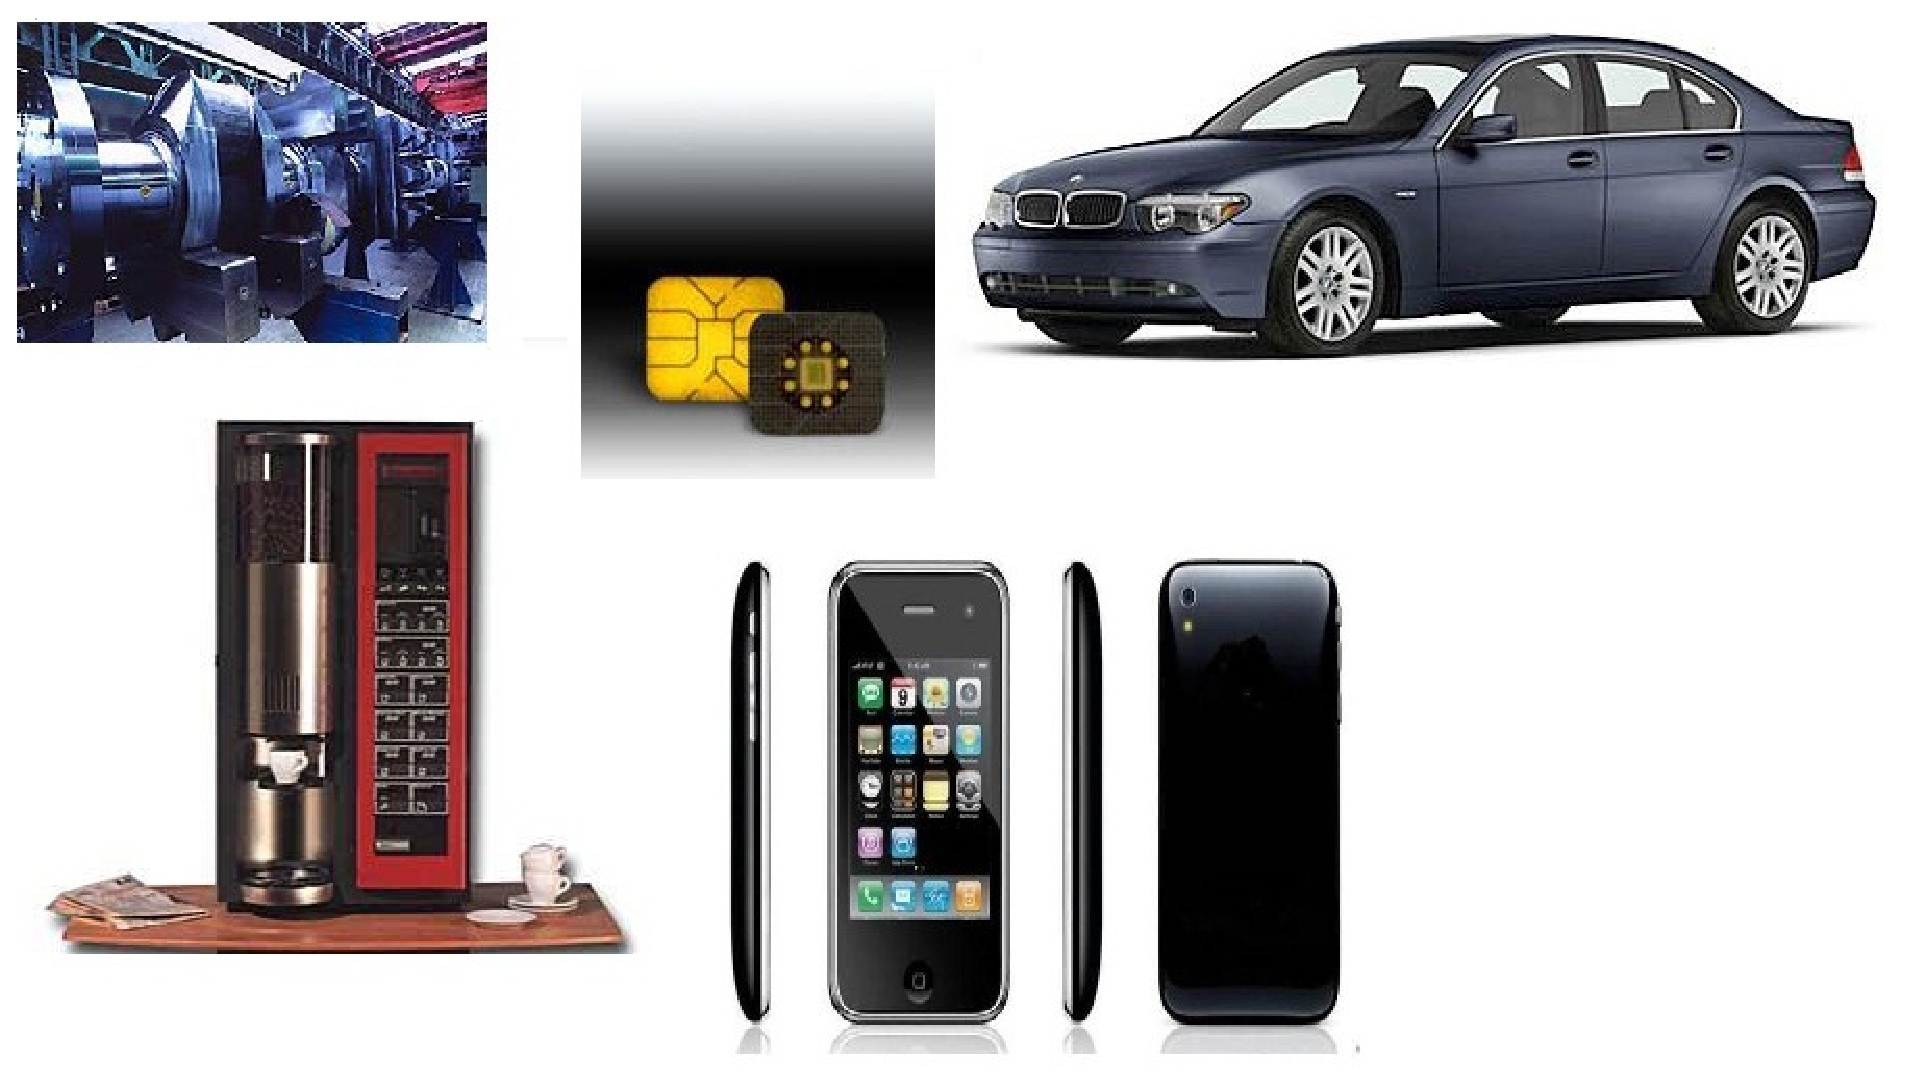
\includegraphics[scale=0.5, width =\columnwidth]{Figures/usos}
\end{center}
  \caption{Example of systems where formal methods are (can be) used .}
  \label{fig:uso}
\end{figure}

In the past, the use of formal techniques in practice seemed to be utopian and unrealizable. 
Among other causes, the notations used to require a high mathematical background in
mathematics and, therefore, they were too complicated for the uninitiated in the topic. 
The techniques did not allow the system to be scalable and the existing tools were
too difficult to use or understand or even there were no tools for a particular 
technique or formalism. In addition, case studies were not convincing enough and, 
therefore, developers could not appreciate the usefulness of formalization. 
However, in the early 90s, it started to glimpse a new way in this area. 
For the specification of software, the industry began to use the language Z \cite{Abrial80} 
in order to obtain rigorous specifications. For hardware verification, major 
companies such as Intel and AMD started to use formal techniques such as \emph{model checking} 
or \emph{theorem proving} to supplement tests on simulators. This led to the description of larger case studies,
which was benefitial for the advance of this area since other developers started to consider the possibility of 
introducing the use of formal techniques into their development processes.
In Figure \ref{fig:uso}, one can observe different systems in which these techniques are currently
used to ensure proper operation. For instance, big companies (e.g Boeing and Airbus)
use formal languages to specify the requirements of the equipment as well as they use 
formal methods to verify the most critical systems in the aircrafts. Moreover, automotive
companies verify the most critical systems ( e.g. brake or airbag systems) using \emph{model checking}. 

The main advantages of using formal methods are:

\begin{itemize}
\item The use of mathematics as a base gives this approach a certain rigour.
\item Identify ambiguity and inconsistencies.
\item Facilitates the construction of consistent and \emph{deadlock-free} systems.
\item Provides customer confidence in the system.
\item There are many tools that support the existing techniques.
\item Find bugs early should save money.
\end{itemize} 

The main disadvantages (or beliefs) that slow the progress of this area are:

\begin{itemize}
\item It is believed that the use of formal methods slows the development process.
\item Many developers think it is difficult to work with formal specifications.
\item It does not guarantee the correctness of the implemented code (only the model
it is based).
\item Increasing system complexity causes an exponential increase
the complexity of the verification.
\end {itemize}

As commented previously, companies can use formal methods along the entire
development lifecycle of a system, both hardware and software. 
Here, we will focus on software since this Thesis studies different standards for building software components. 
Next, we describe the different phases in which designers can apply any formal technique. 

One of the most important part in the development of a system is the requirements specification. 
A specification can be seen as a technical document where the features and services needed 
to build a product are stated. Nevertheless, it can also include information on 
subsequent steps such as verification, validation, testing, etc. Therefore, 
this should be the first part in which the participants should apply formal methods, taking the 
required time to correctly specify the system since a neat and correct specification will influence the 
rest of the proccess.
Anyway, make a proper specification does not guarantee the absence of errors because the 
presence of faults is an intrinsic characteristic of the systems. In this sense, 
the simple act of writing the document helps engineers to find errors in the early stages 
of the development process, helping the company to save  money and time. 
In Figure \ref{fig:coste}, one can observe what is the effect (in money) of finding a bug
in the different phases. As can be observed, the cost of fixing a bug increases as 
we advance in the lifecycle and, therefore, it is recommended to find these bugs as soon as possible. 
In this Thesis, we propose a formal language and its visual model to specify web service compositions 
with distributed resources, but this will be presented in Chapter \ref{chapter:c3}.

\begin{figure}
\begin{center}
  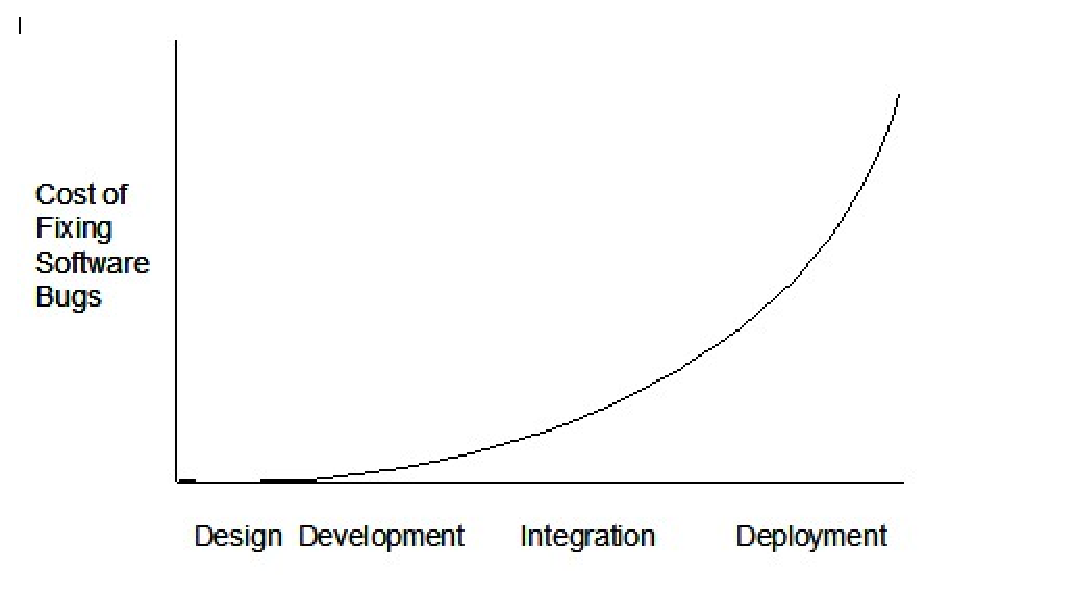
\includegraphics[scale=0.5, width =\columnwidth]{Figures/coste}
\end{center}
  \caption{Cost evolution of fixing a bug.}
  \label{fig:coste}
\end{figure}

In the classic life cycle, the verification and validation phases are performed after the implementation phase, 
but as we have seen in Figure \ref{fig:coste}, it is advisable to detect these errors as soon as possible. 
As expected, it is practically impossible to verify completely all the behaviour of a complex 
system so that the goal of researchers in this area is to check whether certain properties hold in the model. 
The properties of interest will be related to the classical problems of concurrency (\emph{deadlock, mutual exclusion,\ldots}) 
and some aspects directly related to the system itself such as check 
the adherence of it to certain time constraints. For example, in a banking system, 
it is mandatory to ensure that transactions meet the stipulated time for completion 
because if you exceed these restrictions some security issues could come out.

In this sense, one can follow two different ways to perform 
the verification of a system: \emph{Human-directed proof or Automated proof}.
The first one is used when you want to strengthen the knowledge of the system 
rather than completely ensure the correctness of it, and, therefore, it is a person who check the properties manually. 
This variant improves the knowledge of the system, but it is time-consuming and 
error-prone due to the entire process is conducted for a human being. 
In the second approach (\emph{automated proof}) there are also two variants: \emph{automated theorem proving and model checking}. 
The \emph{automated theorem proving } is conducted by a program that tries 
to produce a formal proof of a system from scratch, giving a description of it, 
a set of logical axioms and a set of inference rules. On the other hand, model checking \cite{Clarke99} 
is a technique for verifying finite state concurrent systems. It has a number of advantages 
over traditional approaches that are based on simulation, testing, and deductive reasoning. 
In particular, model checking is normally automatic and usually quite fast. Also, if the design contains an error, 
model checking will produce a counterexample that can be used to pinpoint the source of the error. 
Here, the specification can be expressed in propositional temporal logic propositional 
normally LTL \cite{Pnueli77} or CTL \cite{Henzinger94} or some of its variants, 
and the system is represented as a graph of transitions between states. 
The main challenge in model checking is dealing with the state space explosion problem. 
When dealing with web systems, this problem occurs in systems with many components that can interact with 
each other or systems with data structures that have many different values. 
In such cases the number of global states can be enormous. 
Researchers have made considerable progress on this problem over the last ten years. 
% Typically , the client only available to the engineer high-level representation of the system (usually in natural language ) and the specification of the same , also in natural language. So any \ emph { model checker } ( Spin \cite{Holz04} , UPPAAL \cite {Larsen97}, etc.) Exits with an affirmative answer if the proposed design meets the specification or provides a counterexample to locate where it has the error.

 
\section{Web Services modelling}

Although the Web was initially intended for the exclusive use of human beings, 
many experts believe that it needs to evolve (probably through modular design 
and construction services) to better support for the automation of many tasks. 
The concept of \emph{service} provides a higher level of abstraction to organize 
large-scale applications and build more open environments, helping to develop 
applications with improved productivity and quality with respect to other approaches. 
As services are only a mean for building distributed applications, 
it is required to evaluate the different existing approaches in this area. 
Figure \ref{arch} shows an example of service-based architecture, 
where there are three main parts: a consumer, a provider (the servers) and a set of records, 
where the services are stored. The role of the providers is to publish and/or advertise the 
services offered in the records, where consumers can find and invoke them. 
Current standards that support interactions between web services provide a 
solid foundation for service-oriented architecture. 
The web architecture is a framework that can be reinforced with more 
powerful representations and techniques inherited from other approaches.

\begin{figure}
\begin{center}
  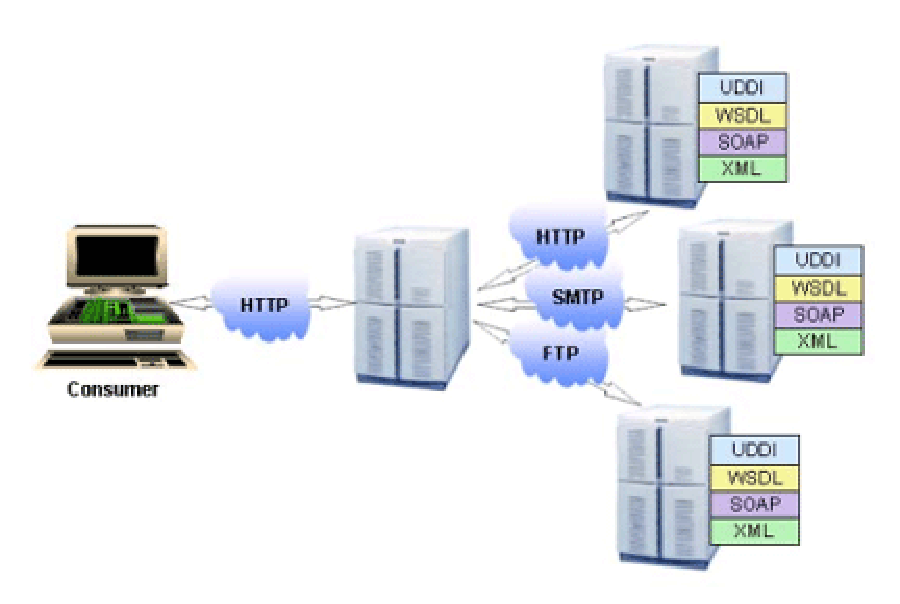
\includegraphics[width =\columnwidth]{Figures/clientserver.eps}
\end{center}
  \caption{Client-server web architecture}
  \label{arch}
\end{figure}

In this way, Service-Oriented Computing (SOC) paradigm promotes the use of services 
for the development of massively distributed applications, trying to achieve the creation of fast, 
low-cost, flexible and scalable applications \cite{Papazoglou2007}. 
Services are the main building block of this paradigm, being these services self-describing and platform-independent. 
Thanks to the use of standards for the description, publication, discovery and invocation, 
the services can be integrated without taking care of the low-level implementation 
details of each service. The aim of SOC is to make possible 
the creation of dynamic business processes and agile applications 
by providing an easy way to assemble application components into a loosely coupled network of services.

To reach the goals of SOC, a Service-Oriented Architecture (SOA) is defined. 
SOA is a software architecture based on the utilization of services, 
being these services provided to the user of the application or to other services in the network. 
This is possible by the use of service interfaces that can be published and discovered. 
SOA is based on a model of roles where every service can play multiple roles. 
For example, a service can offer certain functionality to a user and, at the same time, 
being the consumer of the functionality provided by some other services. 
Such model reduces the complexity of applications and increases their flexibility. 
Although at the beginning of SOA there were several architectures aspiring 
to become SOA standards \cite{Karp2000,Sun1999}, the most successful one was the architecture based on Web Services.

W3C defines a Web Service (WS) in the following way:

\begin{quotation}
	``A Web Service is a software system designed to support interoperable machine-to-machine interaction over a network. It has
an interface described in a machine-processable format (specifically WSDL). Other systems interact with the Web Service in a manner prescribed by its description using SOAP-messages, typically conveyed using HTTP with an XML serialization in conjunction with other Web-related standards.''
\end{quotation}

We can see in this definition that there are two basic standards 
related to Web Services: Web Service Description Language (WSDL) for the definition 
of the service functionality and its properties \cite{W3C2001}, 
and Simple Object Access Protocol (SOAP) for the exchange of 
XML messages between services \cite{W3C2007}. 
There is also an additional standard called Universal Description, Discovery and Integration (UDDI) 
used to create Web Service directories and to search for services 
in the network \cite{OASIS2004}, but this is a bit out of date. The use of these standard protocols is 
the key point to improve the integration between different parties in a web service architecture.

In Figure \ref{Figure1} a possible representation of the web service architecture stack is shown. 
One can see that the three standards described above are only a small part of the stack. 
One also need protocols to define security aspects (ensuring that exchanges of information 
are not modified or forgotten in a verifiable manner and that parties can be authenticated), 
to provide reliable messaging for the exchange of information between parties, 
to specify the collaboration between services when we compose them, 
to individually describe the behaviour of each service in a business process, etc. 
The problem is that whereas the standards for basic services (WSDL and SOAP) 
are widely adopted for their respective purposes, the situation is not very 
clear when we talk about composing services, 
having multiple protocols aspiring to become a standard in this layer.

\begin{figure}[h]
\begin{center}
\psfig{file=Figures/ws-stack.eps,scale=.55}
\end{center}
\caption{Web Service architecture stack.}
\label{Figure1}
\end{figure}

Two different approaches can be followed when we designing web service compositions. 
They are called \textit{orchestration} and \textit{choreography}. 
The former describes the individual business process followed by 
each one of the participants in the composition, 
while the latter describes the composition from a global viewpoint, 
defining the interactions (exchange of messages) happening between the parties, that is, 
how they collaborate in the composition. In Figure \ref{orch}, it is depicted graphically what it the role
of each of them if they are compared with the musicians in an orchestra. Despite these differences, the ideal solution would 
be fusing both approaches in a single language and environment \cite{Papazoglou2007}.

\begin{figure}[h]
\begin{center}
\psfig{file=Figures/orchestra.eps,scale=.5}
\end{center}
\caption{Choreography vs. Orchestration}
\label{orch}
\end{figure}

Anyway, the languages we can use in both cases should accomplish some common goals: 
(i) the capacity of modelling service interactions, including control flow and data constraints, 
(ii) the possibility of specifying exceptional behaviour, 
indicating which errors can happen in the execution of the composition 
and the way of handling these errors, and (iii) the ability to model web service compositions at a high level, 
without taking care of the implementation details of each one of the services.

{\bf Comment: Concluir ventajas y desventajas de cada uno.} 
Choreography on the other hand does not rely on a central coordinator. Rather, each
web service involved in the choreography knows exactly when to execute its operations
and whom to interact with. Choreography is a collaborative effort focused on exchange
of messages. All participants of the choreography need to be aware of the business
process, operations to execute, messages to exchange, and the timing of message
exchanges.
The most recent answer to the integration challenge is the Service Oriented
Architecture (SOA) and the web services technologies. The bottom-up view of the SOA
sees different business applications exposing their functionalities through web services.
Thus we can now access different functionalities of different legacy and new developed
applications in a standard way (through web services). Such access to functionalities is
important because typical companies have a large number of existing applications
which have to be integrated.
Regarding the choreography approach, there are several languages that 
have been designed for that purpose. One of the most popular languages 
is Web Services Choreography Description Language (WS-CDL), 
which specifies the common and complementary observable behaviour of 
all participants in a composition \cite{W3C2005}. 
It is based on XML and describes the peer-to-peer collaborations 
between the composite web services from a global point of view, that is, 
the exchange of messages to achieve a common business goal. 
The aim of this language is allowing the composition of any kind of web services, 
regardless of the platform hosting the service or the implementation language. 
Figure \ref{Figure2} is an example of how WS-CDL can be useful 
for the integration of different kinds of web services.

\begin{figure}[h]
\begin{center}
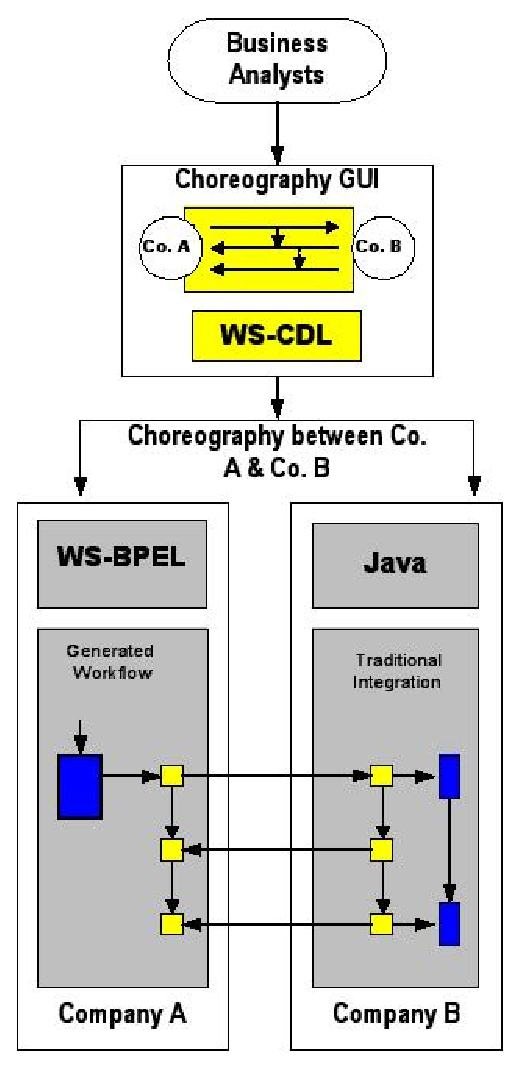
\psfig{file=Figures/WSCDL.eps,scale=.7}
\end{center}
\caption{Integration of Web Services using WS-CDL.}
\label{Figure2}
\end{figure}

A WS-CDL document defines a hierarchy of choreographies, where there is only one top-level choreography, marked explicitly as the \textit{root choreography}. The basic building block of a choreography is the \textit{interaction} element. It indicates information exchanges between participants, possibly including the synchronization of some information values. These interactions are performed when one participant sends a message to another participant in the choreography. When the message exchanges complete successfully, the interaction completes normally. 

We can distinguish two different kinds of \textit{complex activities} inside a choreography: the workunit element and the ordering structures. The \textit{workunit} element specifies a condition that must be fulfilled in order to perform some work and/or the repetition of some work. It completes successfully when the set of activities inside completes successfully. \textit{Ordering structures} are used to combine basic activities and other complex activities in a nested way, expressing the order in which actions are performed within the choreography. There are three ordering structures: The \textit{sequence} ordering structure expresses that the set of activities inside must be executed sequentially. The \textit{parallel} ordering structure indicates that the set of activities inside must be executed concurrently. It completes successfully when all the concurrent activities complete successfully. And the \textit{choice} ordering structure specifies that only one of multiple activities can be executed. If the choice have workunits inside, only the first one in lexical order with a ``true'' guard condition is selected. If there are other activities, there is no way to know which one is selected; it is considered as a non-observable decision.

Different types of exceptions are considered in WS-CDL. Exception workunits can be defined to handle all these exceptions. They may also be used as the mechanism to recover from the exceptions. At least one exception workunit must be defined. The guard of the workunit can be used to specify the particular type of exception we want to handle. Only one exception workunit can match each exception. If multiple exception workunits are defined, the order of evaluating them is based on the order in which the workunits have been defined. When the matching happens, the actions of the matched workunit are executed. If no matching happens and a default exception workunit exists, then the actions of this workunit are executed. Otherwise, the exception is raised in the parent choreography. WS-CDL also allows us to define finalization actions within a choreography that can confirm or cancel the effects of this choreography, so we can use this actions for compensation. 

Next, we introduce the orchestration approach used in this Thesis.

\subsection {WS-BPEL}
In 2002, researchers and engineers of the main companies of the world (IBM, Microsoft, etc.)
realised that the new and rapidly emerging process-oriented approach required the definition of 
a neat and precise language for describing how a set of intecting web services can be included
in a business process. Traditional methods for integration and business process automation 
typically involve embedded logic inside of applications designed 
to meet a specific business need such as ERP, supply chain, or CRM. 
The development, testing, and deployment efforts required 
to change these applications make integration and process changes both costly and complex \cite{}.
To address these issues, proprietary products emerged 
to abstract integration and process automation into a new layer of software tools. 
These software products liberated integration and process tasks from 
the underlying business systems so they could be more effectively changed, managed, and optimized.
The idea and motivation behind almost each new technology and platform for
enterprise application development is to provide an environment where better
business applications can be developed with less effort and these business applications
should closely align to the business processes, which should not be too complex, and
which can be adapted to the changing nature of business processes without too much
effort. Within companies, business applications have to
interoperate and integrate. Integrating different
applications has always been a difficult task for various functional and technology
related reasons \cite{}.

The Business Process Execution Language for Web Services (BPEL4WS), for short BPEL, 
was first conceived in July, 2002 with the release of the BPEL4WS 
1.0 specification. This first draft was initially developed by just three companies, IBM, Microsoft, and BEA. 
This document proposed an orchestration language inspired 
by previous variations such as Web Services Flow Language (WSFL), developed by IBM and XLANG specification language developed
by Microsoft. WSFL was designed by IBM and is based on the concept of directed graphs.
XLANG was designed by Microsoft and is a block-structured language. BPEL combines
both approaches and provides a rich vocabulary for description of business processes. After this first attempt, other major companies such as SAP and Siebel Systems joined the former ones to write
the version 1.1 of the BPEL4WS specification that was released less than a year later, in May of 2003. 
Fortunately, this brand new version received much more attention and vendor support, 
leading to a number of commercially available BPEL4WS-compliant 
orchestration engines \cite{}. Before publishing this release, 
the BPEL4WS specification was submitted to an OASIS 
technical committee in order to be evaluated so that the specification could be developed into an official and open standard.
This technical committee was active from April 2003 to May 2007, 
and, during this time, a lot of contributions and improvements were received. 
In April 2007, WS-BPEL version 2.0 was approved as an OASIS standard. 
As a proof of maturity, more than 37 organizations collaborated to develop WS-BPEL, including representatives of Active Endpoints, Adobe Systems, BEA Systems, Booz Allen Hamilton, EDS, HP, Hitachi, IBM, IONA, Microsoft, NEC, Nortel, Oracle, Red Hat, Rogue Wave, SAP, Sun Microsystems, TIBCO, webMethods, and other members of OASIS \cite{}.
Finally, in January 2008, another OASIS technical committee started 
to define a WS-BPEL extension to emcompass the definition of 
human interactions (``human tasks'') as part of a WS-BPEL process. Figure \ref{bpelevolution} summarises this evolution-

\begin{figure}[h]
\begin{center}
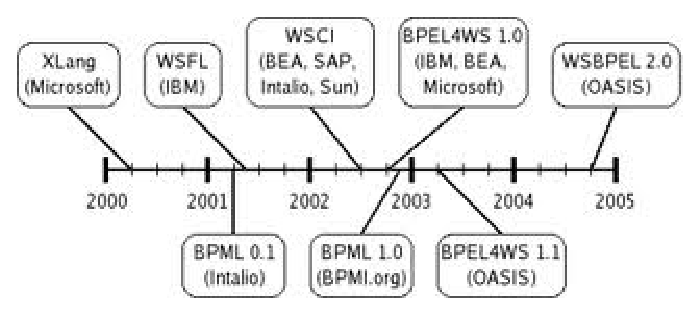
\psfig{file=Figures/bpelhistory.eps,scale=.7}
\end{center}
\caption{WS-BPEL evolution.}
\label{bpelevolution}
\end{figure}

Moreover, there were established ten original design goals associated with the definition of WS-BPEL \cite{wsbpelstandard}:
\begin{itemize}
\item Define business processes that interact with external entities 
through web service operations defined using WSDL, and that 
manifest themselves as web services defined using WSDL. 
\item Define business processes using an XML-based language. 
Do not define a graphical representation of processes or provide any particular design methodology for processes.
\item Define a set of web service orchestration concepts that are meant to be used by both the external (abstract) and internal (executable) views of a business process. Such a business process defines the behavior of a single autonomous entity, typically operating in interaction with other similar peer entities. 
%It is recognized that each usage pattern (i.e., abstract view and executable view) will require a few specialized extensions, but these extensions are to be kept to a minimum and tested against requirements such as import/export and conformance checking that link the two usage patterns.
\item Provide both hierarchical and graph-like control regimes, and allow their use to be blended as seamlessly as possible. This should reduce the fragmentation of the process modeling space.
\item Provide data manipulation functions for the simple manipulation of data needed to define process data and control flow.
\item Support an identification mechanism for process instances that allows the definition of instance identifiers at the application message level. Instance identifiers should be defined by partners and may change.
\item Support the implicit creation and termination of process instances as the basic lifecycle mechanism. Advanced lifecycle operations such as ``suspend'' and ``resume'' may be added in future releases for enhanced lifecycle management.
\item Define a long-running transaction model that is based on proven techniques like compensation actions and scoping to support failure recovery for parts of long-running business processes.
\item Use Web Services as the model for process decomposition and assembly.
\item  Build on Web services standards (approved and proposed) as much as possible in a composable and modular manner.
\end{itemize}

As a result, WS-BPEL along with web services technologies provide now a standardized integration interface 
and a standardized language for the integration of different services as well as for the automation of some tasks. 
Nevertheless, web scenarios are becoming more and more complex since they highly heterogeneous, that is, a lot of different
services from different companies interact jointly to perfom a particular task. In particular, it is known
that business processes change relatively often due to this heterogeneity. Therefore, designers 
do not need only a way to compose a set of services, rather they also
need a way to compose and modify them in the right order and in a relatively 
uncomplicated and straightforward way. Due to this, BPEL is sometimes compared 
to general purpose programming language, but it
is not as powerful as one of the well-known programming language \cite{}. However, 
it is simpler and better suited for business
process definition and, therefore, BPEL must be considered a supplement to
modern languages rather a replacement.

%The first version of BPEL has been developed in August 2002 by BEA, IBM, and
%Microsoft. Since then the majority of vendors have joined which has resulted in several
%modifications and improvements and adoption of version 1.1 in March 2003. In April
%2003, BPEL was submitted to OASIS (Organization for the Advancement of Structured
%Information Standards) for standardization purposes where the WSBPEL TC (Web
%Services Business Process Execution Language Technical Committee) has been formed
%since. This
%has led to even broader acceptance in industry.


%there are two possible ways to compose a set Choreography has not gained support from the
%industry which would be comparable to BPEL \cite{}.
%This is where the BPEL (Business Process Execution Language for Web Services, also
%WS-BPEL or BPEL4WS) becomes important. BPEL allows composition of web services
%and is thus the top-down approach to SOA ? the process oriented approach to SOA.
%Let us have a closer look at a typical BPEL process. First, the BPEL business process
%receives a request. To fulfill it, the process then invokes the involved web services and
%finally responds to the original caller. Because the BPEL process communicates with
%other web services, it relies heavily on the WSDL description of the web services
%invoked by the composite web service.

After briefly introduce its history and design goals, we discuss next its technical details. 
BPEL is therefore an orchestration
language in the sense that it is used to define the composition
of services from a local viewpoint, describing the individual
behaviour of each participant. Choreography is covered by other standards,
such as WS-CDL (commented previously). BPEL is designed to support the description of both behavioural service interfaces and executable
service-based processes \cite{OuyangVABDH07}. A behavioural interface (known as abstract process) is a specification of the
behaviour of a class of services, capturing constraints on the ordering of messages to be sent to and
received from a service. An executable process defines the execution
order of a set of activities (mostly communication activities), the partners involved in the process, the
messages exchanged between partners, and the events and exception handling specifying the behaviour
when specific events or faults occur. In Figure \ref{bpelexample}, we can observe an example of the typical business process
of a travel agency.

\begin{figure}[h]
\begin{center}
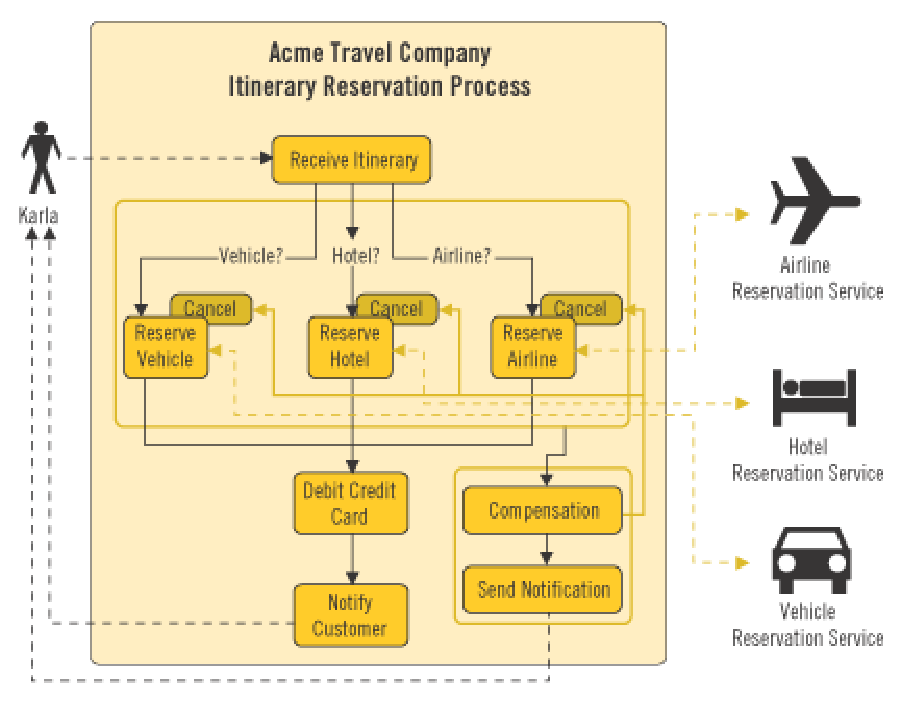
\psfig{file=Figures/bpelexample.eps,scale=.7}
\end{center}
\caption{Example of a business process workflow.}
\label{bpelexample}
\end{figure}

According to the standard of WS-BPEL, an  abstract process is a partially specified process that is not intended to be executed
and it must be explicitly declared as ``abstract''. As its name indicates, 
an abstract process may hide some of the required 
operational details expressed by an executable artifact.
All the constructs of executables processes are made available to abstract processes
and, consequently, they share the same expressive power \cite{}. 
Therefore, the main different between an abstract and a executable processes is 
that the second one contains the exact details of business processes and, consquently,
it is intended to be executed in an orchestration engine, whereas the first one serve a descriptive role,
defining the message exchange between the parties involved. Specifically, an abstract process is usually use to 
describe the observable behavior of some or all of the services offered by an
executable process and/or to define a process template that contains domain-specific best practices. 
Such a template can be seen as a design-time representation of the process logic, excluding execution details to be
completed when mapping to an executable process.
In most cases BPEL is used for
executable processes \cite{}.
Moreover, the definition of conceptual model in which one can define an abstract or an executable
process is a key feature of WS-BPEL since the processes execute and interact with their
partners in a consistent way regardless of the supporting platform or programming model used
by the implementation of the hosting environment, unlocking the potential of
web services because it allows the development of tools and other technologies that greatly
increase the level of automation and thereby lower the cost in establishing cross enterprise
automated business processes. In addition to this, abstract process ensures the level of privacy required by the 
companies since the implementation of the service is hidden to the other participants. 

In detail, WS-BPEL is an XML-based language which
supports the web services technology stack, including SOAP, WSDL, UDDI and so on. 
It defines a model and a grammar for describing the behavior of a business process
based on interactions between the process and its partners as well as the order of these interactions. 
The interaction with each partner is performed through web service interfaces, 
and the structure of the relationship at the interface level
is encapsulated in what is called a partnerLink. WS-BPEL also introduces 
mechanisms for dealing with business exceptions and faults. Moreover, WS-BPEL
introduces a mechanism to define how activities have to be compensated in cases 
where exceptions occur or a partner requests reversal.
A WS-BPEL process is a reusable definition that can be deployed in different ways and in
different scenarios, while maintaining a uniform application-level behavior across all of them.


\begin{figure}[h]
\begin{center}
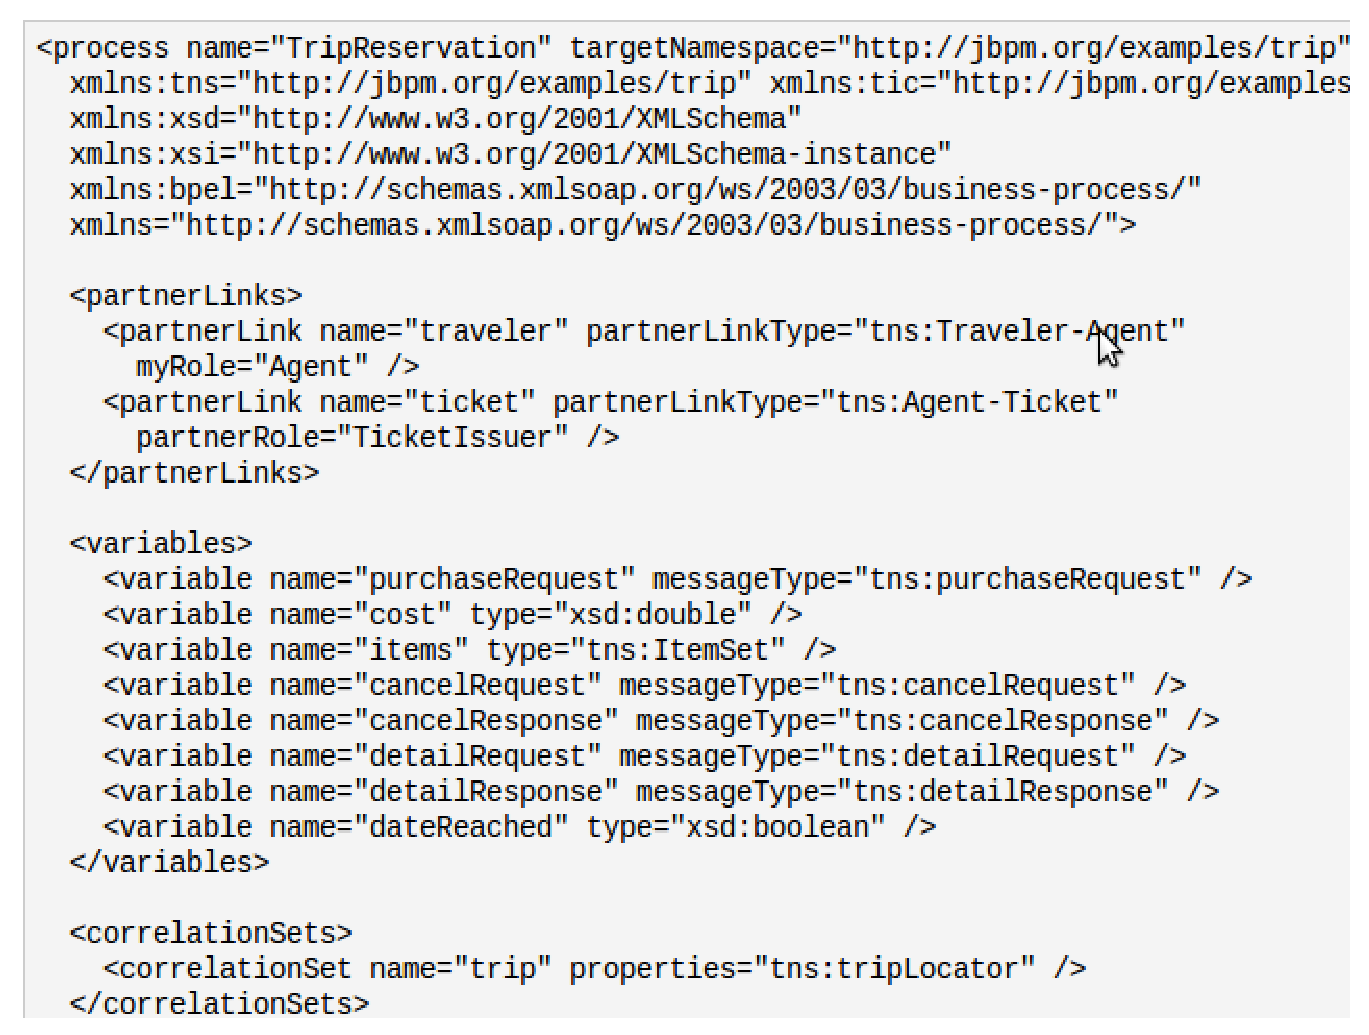
\psfig{file=Figures/bpelcode.eps,scale=.5}
\end{center}
\caption{WS-BPEL code.}
\label{bpelcode}
\end{figure}

In Figure \ref{bpelcode}, we can observe a piece of the BPEL code for a booking process. 
BPEL processes use {\em variables} to temporarily store 
data. Variables are therefore declared on a process or on a scope 
within that process. Also, 
it provides \emph{basic} or \emph{structured} to declare the process logic. 
\emph{Basic activities} are those which describe the elemental 
steps of the process behaviour \cite{}: 
\begin{itemize}
\item The activity \emph{assign} is used to assign data to the variables defined in the process. 
This activity can be used to copy data from one variable to another as well as to
populate new data in a variable using expressions. As usual, expressions are constructed using 
variables and constants. 
\item The activity \emph{empty} is devoted to be used as an activity that does nothing. For instance, one can
decide to capture an exception and do nothing to handle it. Another use of \emph{empty} is
to provide a synchronization point in a parallel activity.
\item The activity \emph{wait} specifies a particular delay or deadline. 
\item To invoke a web service of service provider, WS-BPEL offers the activity {\em invoke}. 
Normally, this activity is used to request an operation in a service. This operation is usually 
a basic activity in the provider. Operations can be of two types: request-response or one-way.
One-way consist of sending a message (some variables can be enclosed) so that no response is expected
as part of the operation, whereas a request-response invocation requires a message back. Evidently, this
response message can be used to notify the sender about a fault during the operation. A more detailed
explanation will be provided in Chapter \ref{chapter:c3}. 
\item A \emph{receive} activity is necesary to receive the message sent in the invoke activity.
messages, the portType (optional) and operation that it expects the partner to invoke. The
value of the partnerRole in the partnerLink is not used when processing a <receive> activity.
In addition, it specifies a variable, using the variable attribute, to
store the message the operation to be requested. In many cases, this activity is the first part of the process.
\item The \emph{reply} activity is used to respond to a request previously accepted through an
inbound message activity. For instance, it can be used in conjunction with the receive activity
to respond to the invocation of a service. Clearly, it is only meaningful
for request-response interactions, but a one-way ``response'' can be sent by invoking the
corresponding one-way operation on the sender. Finally, it may specify a
variable attribute that references the variable that contains the message data to be sent.
\item The activity \emph{throw} is used to signal an internal fault explicitly.
\item The activity \emph{exit} is used to immediately end the process instance.
\item WS-BPEL provides the user with the ability to declare new activities that are
not contemplated in the specification. This is done using the \emph{extension activities}. This
extension is not explicitly contemplated in the theory of this Thesis, although they are required
to implement the theory in an orchestration engine.
\item Finally, using the activity \emph{rethrow} in a fault handler, it is possible to rethrow a fault.
For instance, this activity is useful when the situation that causes the fault is not solved after
the completion of the fault handler and, therefore, it is needed to redo this handler to check if the
situation has been solved afterwards.
\end{itemize}  

On the other hand, \emph{Structured activities} encode the control-flow logic of the process.
The set of structured activities defined in the standard are the following:
\begin{itemize}
\item The activity \emph{sequence} includes a set of activities that are performed sequentially in the
order in which they appear in the structure. It ends
when the last activity in the sequence has finished.
\item The activity \emph{flow} provides concurrency and synchronization, creating 
a set of concurrent activities directly nested within the process and it enables
synchronization dependencies between activities that are nested to it. A more detailed explanation
of how this activity works is given in Chapter \ref{chapter:c3}.
\item The activity \emph{if} specifies conditional behavior. As usual, the activity consists of an ordered list of one or
more conditional branches defined by the ``if'' and optional ``elseif'' elements, followed by an
optional ``else'' element.
\item The activity \emph{while} provides conditional repetitive behaviour.
\item \emph{RepeatUntil} provides the repeated execution of a contained activity. The difference with
the activity while is that the inner activity is executed at least once.
\item The activity \emph{pick} waits for the occurrence of exactly one event from a set of events, and then
executes the activity associated with that event. After an event has been selected, the other events
are no longer accepted by that ``pick''. Moreover, a deadline for the occurrence of such events can be established
in such a way if this deadline experies the pick activity ends. This structure has some similarity the choice operator in
a process algebra althoudh with a predefined timeout. 
In WS-BPEL, it can be compared with a set of receive activities that run in parallel, where just only one can be executed,
and a common deadline for the execution of these receive activities is set (to this end, the wait activity can be used).
\item Lastly, the standard offeres an activity (forEach) to execute the contained activity a predefined number of times that
is expressed in the definition of the activity.
\end{itemize}


\section{Heterogeneous Distributed Systems: Grid/Cloud Computing}

In 1943, the president of IBM, Thomas J. Watson, predicted:

\begin{center}
``I think there is a world market for about five computers''
\end{center}

In recent times, this phrase has been widely discussed since some authors
consider that it is an clear example of failed prediction. Nevertheless, with the advent of new computational 
such as Grid and Cloud Computing, some authors argue that it will become a reality soon. In addition,
other authors consider that this phrase is completely true nowadays since there five big companies that
are monopolising the world market \cite{}.

Thanks to the fast development of society, daily basic services such as water, electricity, gas and telephone services 
are commonly supplied to citizens so that everybody can have 
immediate access to them in developed countries. Today, these services 
known as ``utility'' services since customers are charged according to the consumption. In 1969, Leonard Kleinrock, one of the leading scientists of the American ARPANET agency, said: ``Today, computer networks are in their infancy, but as they grow and become more sophisticated we will see the rise of the \emph { Utility computing}. It is amazing how in 1969 a scientist could already see the usefulness of computers and the advent of a distributed computing model that would be based on providing services and paying for them. What makes this statement more fascinating is that this year is when the Internet was born. The first version only connected 2 computers worldwide, but this person was already thinking that someday the Internet could connect millions of computers into a single network. This vision of computing (based on a model of on demand service provisioning) anticipated the massive transformation of the computer industry in the XXI century. 

Thus, major companies such as Google, Amazon or Microsoft are introducing it in their business model. Moreover, it
is often confused with Cloud and Grid Computing. Utility Computing 
is the underlying business model for a Grid or Cloud infrastructure, i.e. it
can be seen as a mean of charging customers  for computing services so that 
users pay only for the consumption, whereas the costs associated with the production and distribution of computing services 
will be undertaken by the provider. As happens with revolutionary software, 
protocols or any computer-related paradigm, Cloud Computing must undergo 
a series of steps to check if all benefits 
that providers are promising really serves companies to save costs and enhance the competitiveness. 
In this sense, Larry Ellison, founder and CEO of Oracle, believe that Cloud Computing 
is nothing more than a new way of naming what companies have been doing so far \cite{abovetheclouds}: 
\begin{quote}
``The interesting thing about Cloud Computing is that we have redefined Cloud Computing 
to include everything that we already do\ldots I do not understand what we would do differently in the light of Cloud
Computing other than change the wording of some of our ads.''
\hspace{5cm}\emph{Larry Ellison, quoted in the Wall Street Journal, September 26, 2008.}
\end{quote}
Many researchers have tried to define the term ``Cloud Computing'' without reaching 
a standard definition. For instance, Buyya et al. \cite{} define a cloud system as:
\begin{quote}
``A cloud is a parallel and distributed system consisting of a collection of 
virtualized and interconnected computers that have been provisioned dynamically 
and they are presented as a single computational resource based on service level agreements (SLAs) 
established by negotiation between the service provider and the consumer.''
\end{quote} 

In \cite{vaq09} one can find up to 21 different definitions of Cloud computing. For instance, Luis M. Vaquero et al. defines the Cloud as:
\begin{center}
\emph{``The Cloud is a large and easy to use container of virtualized resources 
(such as hardware, services, development platforms \ldots). These resources can be 
dynamically reconfigured to fit into a variable load (scale), allowing also the optimal use of these resources. 
This service is exploited through pay-per-use model that is guaranteed by agreements.''}
\end{center} 

{\bf Meter un par de p�rrafos de Grid}

Finally, the main difference between a Cloud-oriented and a Grid-oriented system relies in the virtualisation of resources. 
In a Grid infrastructure, users do not share in real-time the resources allocated to them, 
whereas in a Cloud infrastructure the virtualisation is essential in order to serve more users,
thus getting the savings promised by suppliers \cite{}.

\section{Web services vs. Grid/Cloud Computing}

As we know , our research group has focused its research on developing a methodology to build and test systems with time constraints using formal techniques . In recent years , this methodology has been applied in the area of ??Web services, more specifically, that these services meet the task entrusted to them and automatically coordinate for conducting a more general work . The problem we are having is that web services as had a boom a few years ago , many research groups focused their studies in this field and therefore there are many researchers proposing new approaches and this has meant that there are certain parts BPEL or WS -CDL are quite studied. Thus, a system is emerging where formal methods can play an important role and where our group can benefit from their vast experience both as formalizing web services , cloud computing . This new paradigm , as discussed above, is living his season correctly right now and big companies like Google , IBM, Microsoft have decided to step forward and bet heavily on cloud computing . In addition , many governments are interested in migrating services to the cloud to reduce costs and enable scalability when they needed. For example , one must ask if it is necessary for the Tax Agency have large data centers where demand for services by citizens grows only at the time of the statement of income. Probably the answer is yes because you do need to store all that data and give some confidence that your tax data will not fall into the hands of people with no good intentions , but all need to calculate whether you can outsource to save costs equipment or could even create a private cloud between all agencies that work with the public agency to share resources and information . In this sense, these systems where security , privacy and availability are a nonnegotiable requirement is where we focus part of our investigations and try to improve any component of the cloud architecture presented in the previous section. For example , most research groups develop tools, but the test phase does not exist or is devoted little time. Last week we met with one of the leading researchers in the field of Grid / Cloud Computing , Karim Djemame , and it told us that the main problem I had was that they did not know specifically that worked well your tool and I was quite interested in the check your tool. \ \


On the other hand , here are some differences between web services and grid / cloud computing to see where to apply our expertise in this system are listed . First, we can consider that Web services are themselves software offered as a service ( SaaS ) , although there are some differences between the two approaches , eg standardization. Therefore, this software could be composed of a set of services , probably communicated via the Internet , and which coordinate to perform a certain task. So far , nothing new, but the main difference lies in virtualization, since different services provided by the cloud are performed in virtual machines rather than directly on a server such as the case of the web service , so that the concurrency in the system is higher. \\

Another difference is the persistence of the data. If we coordinate multiple web services to perform sums the only way that they can store the result is storing it in the database , however , there is an approach called WSRF (Web Services Resources Framework) has been standardized and that resolves this problem . In this framework each Web service is associated with a resource or more of the system so that you can interact with the service and decide which resource access . The main advantage is that all services are defined in WSDL ( Web Services Description Language ) and communication , addressing, etc. . is standardized , so that the cooperation between such systems is simple . Another advantage is that the user can decide which resources interacts with . So , we could add a bottom layer in our methodology that would allow the definition of web services with resources and once verified that the system is correct, these web services deployed on physical machines. This approach fit perfectly with our research because it uses web services with resources and these resources are time restrictions to prevent a user from system-wide . \\

Also, we can see that cloud computing could be seen as a layer to be placed under the web services , since you can use these to access the resources , but we must emphasize that the cloud is not only providing software as a service, but there are infrastructure and platform as a service , which the web services can not cover . That is, a part of cloud computing (SaaS ) can be compared directly with web services, but the other two parties have nothing to do , so it would be like comparing the TCP / IP protocol with the architecture of a PC , although necessary that both approaches (web services and cloud computing) converge to the growth of both paradigms , like grid computing and web services converged on WSRF . \\



\subsection{Web Services Resource Framework(WSRF)}

La arquitectura que presentan los servicios web ha sido ampliamente aceptada como medio para estructurar las interacciones existentes entre los servicios que forman parte de un sistema distribuido y que colaborar para conseguir un objetivo com�n. En la actualidad, los desarrolladores requieren a los entornos una mayor estandarizaci�n para facilitar interoperatividad adicional entre dichos servicios, pero hasta mediados de 2004 ning�n grupo de investigaci�n o grupo de expertos se hab�a planteado seriamente la idea de proponer un est�ndar para modelar la comunicaci�n entre servicios web que poseen recursos persistentes asociados. As�, en Enero de ese a�o, varios miembros de la organizaci�n \emph{Globus Alliance} y de la multinacional inform�tica IBM definieron, con la ayuda de expertos de empresas como HP, SAP, Akamai, etc., la especificaci�n de los documentos que deber�an producirse en este modelo y la base de una arquitectura inicial. Estos documentos fueron enviados a la organizaci�n encargada de su estandarizaci�n, OASIS, en Marzo de 2004. En un principio, se formaron dos comit�s que se encargar�an del estudio y desarrollo de ciertas partes de este nuevo est�ndar. Por un lado, estaba el \emph{WSRF Technical Committee} que gestionaba cuatro especificaciones: \emph{WS-ResourceProperties, WS-ResourceLifetime, WS-ServiceGroup, y WS-BaseFaults}. Por otro lado, el \emph{WSN Technical Committee} se encargaba de las especificaciones: \emph{WS-BaseNotification, WS-Topics, y WS-BrokeredNotification}. \\

WS-Resource Framework est� inspirado en el trabajo realizado previamente por el \emph{Global Grid Forum's Open Grid Services Infrastructure (OGSI) Working Group} \cite{Foster03}. M�s concretamente, puede ser visto como una sencilla refactorizaci�n de los conceptos e interfaces desarrollados en la especificaci�n \emph{OGSI V1.0}, de manera que explota los recientes desarrollos en el �rea de los servicios web (por ejemplo, WS-Addressing). \\

El objetivo de este trabajo es introducir los conceptos fundamentales para la gesti�n y destrucci�n de servicios web persistentes, es decir, servicios web que llevan asociados recursos donde guardar los estados de los mismos, ya que hasta la aparici�n de esta aproximaci�n, los servicios web eran considerados ``\emph{stateless}'' y, por tanto, no pod�an almacenar temporalmente datos o resultados de sus operaciones de una manera sencilla para el usuario, ya que era necesario almacenarlos en una base de datos ajena al servicio. En este enfoque, es necesario codificar la relaci�n entre el servicio y el recurso en t�rminos de patrones utilizando una serie de tecnolog�as ampliamente estudiadas, como, por ejemplo, el WS-Addressing y, tambi�n, ser� necesario hacer sus propiedades accesibles desde el exterior a trav�s de un interfaz. En este sentido, llamaremos \emph{WS-Resource} a la asociaci�n entre un servicio web y un recurso persistente.  


\subsection{Introducci�n}

WS-Resource Framework \cite{Ban06} es una especificaci�n, desarrollada por OASIS y algunas de las empresas inform�ticas m�s pioneras, cuyo prop�sito es definir un marco gen�rico para el modelado y acceso a recursos asociados a servicios web, as� como las relaciones entre dichos recursos en un entorno Grid/Cloud. Esta aproximaci�n est� compuesta por un conjunto de especificaciones que definen la representaci�n del WS-Resource en los t�rminos que especifican los mensajes intercambiados y los documentos XML relacionados. Asimismo, incluye mecanismos que describen el medio para consultar el estado de un recurso y la descripci�n del servicio, que forman conjuntamente la definici�n de un WS-Resource. Adem�s, definen los pasos necesarios para hacer el estado de un servicio web accesible a trav�s de su interfaz (descrita en WSDL).\\

Normalmente, las interfaces de los servicios web proporcionan al usuario la posibilidad de acceder y manipular el estado del mismo, como, por ejemplo, valores de datos que evolucionan por la interacci�n entre varios servicios. En otras palabras, los intercambios de mensajes que se implementan en el comportamiento de los servicios tienen como objetivo permitir el acceso a estos recursos persistentes. Sin embargo, la noci�n de recursos persistentes que subyace en la implementaci�n de los servicios no es tan evidente en la definici�n de la interfaz \cite{Fost04}. Los mensajes que estos servicios env�an y reciben implican (o animan al programador a inferir) la existencia de un tipo de recurso asociado. Por tanto, es deseable que se definan est�ndares que permitan el descubrimiento, creaci�n, introspecci�n, interacci�n y destrucci�n de dichos recursos y que la forma elegida para llevar a cabo esta misi�n sea lo m�s interoperable posible. Estas observaciones han motivado la aparici�n de la propuesta comentada anteriormente, WS-Resource, para modelar estados en el contexto de los servicios web. Un WS-Resource se define como la composici�n de un servicio web y sus recursos persistentes asociados, esto es, \emph{(i)} expresado como una asociaci�n de un documento XML con un tipo definido con uno o varios \emph{portTypes} (un servicio podr� jugar un determinado rol si implementa todos los \emph{portTypes} que comprenden ese rol) y \emph{(ii)} direccionado y accedido de acuerdo al patr�n del recurso impl�cito, una derivaci�n de las \emph{Endpoint References} del WS-Addressing. Una \emph{Endpoint Reference} estar� compuesta por: Uniform Resource Identifier (URI), par�metros del mensaje que se envi� para solicitar el env�o de la \emph{Endpoint Reference} y datos relativos a la interfaz que se usa. En este intercambio, el identificador del recurso persistente es encapsulado en una \emph{Endpoint Reference} y usado para identificar al recurso en cualquier intercambio de mensajes entre los servicios que formen la coreograf�a. As�, WSRF permite declarar, acceder, monitorizar y destruir WS-Resources mediante mecanismos convencionales, lo que facilita la tarea de gesti�n, ya que no es necesario hacer m�s dif�cil la l�gica de decisi�n del servicio propietario del recurso para procesar los mensajes de gesti�n. Estos mecanismos convencionales componen cinco especificaciones t�cnicas que definen los medios por los cuales:

\begin{itemize}
\item Se destruye un WS-Resource, ya sea de manera s�ncrona con respecto a una petici�n expl�cita de destrucci�n o, a trav�s de un mecanismo basado en tiempos (scheduled). Adem�s, es posible declarar unas caracter�sticas espec�ficas  de los recursos (WS-ResourceProperties) que podr�an ser utilizadas para inspeccionar y monitorizar el tiempo de vida de dicho WS-Resource (WS-ResourceLifetime).
\item  Se definen los tipos de WS-Resource, que est�n compuestos por la interfaz de la descripci�n del servicio web (WSDL) y por un documento XML de propiedades del recurso. Por otro lado, el estado del WS-Resource puede ser consultado y modificado a trav�s del intercambio de mensajes (WS-ResourceProperties)
\item Un Endpoint Reference (WS-Addressing) puede ser renovado cuando su informaci�n de direccionamiento ha caducado o ha dejado de ser v�lida por alg�n error (WS-RenewableReferences).
\item Adem�s, se define la capacidad de implementar entornos heterog�neos como colecciones de servicios web, sean o no WS-Resources (WS-ServiceGroups).
\item La notificaci�n de errores puede ser m�s estandarizada al usar tipos XML Schema para definir los fallos base y definir reglas que muestren c�mo esos fallos son usados y extendidos (WS-BaseFaults).
\end{itemize}   

\subsection{WS-ResourceProperties}

Como se ha comentado anteriormente, WSRF utiliza una especificaci�n concreta para definir las propiedades del WS-Resource. Este recurso estar� compuesto por la definici�n de la interfaz en WSDL y un documento XML (Resource Properties Document) que especifica las propiedades del mismo, por ejemplo, el tama�o de disco, la capacidad del procesador, etc., de tal manera que si queremos acceder, modificar o actualizar este documento debemos utilizar una serie de mensajes preestablecidos en la especificaci�n. Las operaciones que se pueden hacer son las siguientes:

\subsubsection{GetResourceProperty}
Esta operaci�n como su propio nombre indica permite al servicio web que realiza la petici�n recuperar el valor de una {\bf �nica} propiedad del documento de propiedades. Para aclarar m�s los conceptos se define el siguiente ejemplo. \\


Dado el documento de propiedades:

\lstset{language=XML, numbersep=5pt,basicstyle=\small, frame=single}
\begin{lstlisting}
...
<GenericDiskDriveProperties 
xmlns: tns=``http://example.com/diskDrive'' >
  <tns:NumberOfBlocks>22</tns:NumberOfBlocks>
  <tns:BlockSize>1024</tns:BlockSize>
  <tns:Manufacturer>DrivesRUs</tns:Manufacturer>
</GenericDiskDriveProperties>
...
\end{lstlisting}

Una posible petici�n puede ser:

\lstset{language=XML, numbersep=5pt,basicstyle=\small, frame=single}
\begin{lstlisting}
...
<s12:Body>
  <wsrp:GetResourceProperty 
    xmlns:tns=``http://example.com/diskDrive''>
     tns:NumberOfBlocks
  </wsrp: GetResourceProperty>
</s12:Body>...
\end{lstlisting}

\subsubsection{GetMultipleResourceProperties}
Este m�todo es equivalente al anterior, pero para acceder a m�s de una propiedad del documento en el mismo mensaje, es decir, se utiliza para evitar congestionar la red. El mensaje enviado ser�a:


\lstset{language=XML, numbersep=5pt,basicstyle=\footnotesize ,frame=single}
\begin{lstlisting}
...
<wsrp:GetMultipleResourceProperties
 xmlns:tns=``http://example.com/diskdrive''>
 <wsrp:ResourceProperty>tns:NumberOfBlock</wsrp:ResourceProperty>
 <wsrp:ResourceProperty>tns:BlockSize</wsrp:ResourceProperty>
</wsrp:GetMultipleResourceProperties>
...
\end{lstlisting}

\subsubsection{SetResourceProperties}
Este m�todo se utiliza para realizar cambios en el documento de propiedades. Existen 3 tipos de cambios:

\begin{itemize}
\item Insert: Permite a�adir nuevas propiedades en el documento.
\item Update: Se utiliza para actualizar el valor de alguna propiedad.
\item Delete: Elimina propiedades del documento.
\end{itemize}

Un posible ejemplo de petici�n ser�a:

\lstset{language=XML, numbersep=5pt, basicstyle=\small,frame=single}
\begin{lstlisting}
...
<s12:Body>
 <wsrpw:SetResourceProperties
        xmlns:tns=``http://example.com/diskdrive''>
   <wsrp:Update>
    <tns:NumberOfBlocks>143</tns:NumberOfBlocks>
   </wsrp:Update>

   <wsrp:Delete resourceProperty=``tns:Manufacturer''/>

   <wsrp:Insert>
    <tns:someElement>42</tns:someElement>
   </wsrp:Insert>

 </wsrp:SetResourceProperties>
</s12:Body>
...
\end{lstlisting}


El documento de propiedades quedar�a con el siguiente formato:

\lstset{language=XML, numbersep=5pt, frame=single}
\begin{lstlisting}
...
<GenericDiskDriveProperties
  xmlns:tns=``http://example.com/diskDrive''>
  
  <tns:NumberOfBlocks>143</tns:NumberOfBlocks>
  <tns:BlockSize>1024</tns:BlockSize>
  <tns:someElement>42</tns:someElement>

</GenericDiskDriveProperties>
...
\end{lstlisting}

\subsubsection{QueryResourceProperties}
Como su propio nombre indica, este m�todo se utiliza para realizar consultas sobre propiedades del recurso. Por ejemplo si queremos saber si el n�mero de bloques es mayor que 20 y el tama�o de bloque es 1024 realizar�amos la siguiente consulta:

\lstset{language=XML, numbersep=5pt, frame=single}
\begin{lstlisting}
...
<s12:Body>
 <wsrp:QueryResourceProperties>
  <wsrp:QueryExpression
   Dialect=``http://www.w3.org/REC-xpath-19991116''>
    boolean(/*/NumberOfBlocks>20 and /*/BlockSize=1024)
  </wsrp:QueryExpression>
 </wsrp:QueryResourceProperties>
</s12:Body>
...
\end{lstlisting}

\newpage
La respuesta que env�a el otro servicio es:


\lstset{language=XML, numbersep=5pt, frame=single}
\begin{lstlisting}
...
<s12:Body>
 <wsrp:QueryResourcePropertiesResponse>
   true
 </wsrp:QueryResourcePropertiesResponse>
</s12:Body>
...
\end{lstlisting}


\subsection{WS-Base Faults}
El dise�ador de un servicio web normalmente utiliza interfaces definidas por otros, por lo que un m�todo que estandarizase el formato de los mensajes de notificaci�n de errores facilitar�a la labor de los desarrollares. �ste es el objetivo de WS-BaseFaults. Los mensajes de fallos en WSRF tienen el siguiente formato:


\lstset{language=XML, numbersep=5pt, frame=single}
\begin{lstlisting}
...
<BaseFault> 
  <Timestamp>xsd:dateTime</Timestamp> 
  <OriginatorReference> 
    wsa:EndpointReferenceType 
  </OriginatorReference> ? 
  <ErrorCode dialect=``anyURI''>xsd:string</ErrorCode>? 
  <Description>xsd:string</Description> * 
  <FaultCause>wsbf:BaseFault</FaultCause> * 
</BaseFault>
...
\end{lstlisting}
donde:

\begin{itemize}
\item Timestamp: Hora exacta cuando el fallo ha ocurrido.
\item OriginatorReference: Direcci�n en formato WS-Addressing del servicio que ha generado el fallo.
\item ErrorCode: C�digo de error para ser utilizado por sistemas de informaci�n de fallos, por ejemplo, POSIX errno.
\item Description: Explicaci�n de la causa del fallo (en lenguaje natural).
\item FaultCause: Causa t�cnica del fallo. 
\end{itemize}

\subsection{WS-ServiceGroup}
Esta especificaci�n permite crear grupos que comparten una serie de propiedades en com�n, es decir, agrupar diferentes servicios web que tienen comportamientos similares.

\subsection{WS-ResourceLifetime}

El tiempo de vida de un WS-Resource se define como el per�odo que transcurre entre su instanciaci�n y su destrucci�n. La misi�n de esta especificaci�n es estandarizar el proceso de destrucci�n de un recurso y definir mecanismos para monitorizar este ciclo de vida, pero lo que no se define es c�mo crear el WS-Resource. Generalmente, en los sistemas distribuidos, los clientes s�lo quieren tener un recurso por un determinado intervalo de tiempo, aunque en muchos escenarios es m�s apropiado para el cliente que se produzca la inmediata destrucci�n del recurso. Otro ejemplo claro de uso se presenta cuando el cliente quiere suscribirse a un servicio por un cierto tiempo y quiere que despu�s de este tiempo se destruya dicha uni�n. Como se coment� en la introducci�n, existen dos formas de destruir un recurso: inmediata, mediante un mensaje expl�cito o temporizada, mediante un mensaje que activa o gestiona un timer. 

\subsubsection{Destrucci�n inmediata}
Para la destrucci�n inmediata s�lo hace falta poner \emph{$<wsrl:Destroy/>$} dentro del cuerpo ($<Body>$) del mensaje SOAP que se env�a al servicio que gestiona el recurso y dicho servicio responder con \emph{$<wsrl:DestroyResponse/>$} dentro del cuerpo (\emph{$<Body>$}) del mensaje SOAP de respuesta.

\subsubsection{Destrucci�n temporizada}

En este caso, el WS-Resource tiene asociado un tiempo de terminaci�n que define el tiempo despu�s del cual se espera que el recurso haya sido destruido y, razonablemente, se espera que antes del mismo el recurso est� disponible. A continuaci�n se muestra un ejemplo de c�mo determinar el tiempo de terminaci�n de un recurso:

\lstset{language=XML, numbersep=5pt, frame=single}
\begin{lstlisting}
...
  <s12:Envelope
     <ex:ResourceDisambiguator>
      uuid:ba32-8680cace43f9
     </ex:ResourceDisambiguator>
     <s12:Body>
      <wsrl:SetTerminationTime>
       <wsrl:RequestedTerminationTime>
        2001-12-31T12:00:00
       </wsrl:RequestedTerminationTime>
     </wsrl:SetTerminationTime>
     </s12:Body>
  </s12:Envelope>
...
\end{lstlisting}



Como podemos observar el servicio que solicita la destrucci�n puede indicar la hora de destrucci�n y la hora actual (para evitar desajustes por la forma de representar la zona horaria). Una vez que CurrentTime alcanza el valor TerminationTime, el recurso se destruye sin ninguna intervenci�n m�s y se notifica al emisor del mensaje de destrucci�n que el recurso deja de estar disponible. Existe otro mensaje que se manda desde el receptor al emisor para comunicarle que ha recibido la petici�n de cambio.  \\

Sin embargo, puede darse la situaci�n de que haya m�s de un servicio utilizando el recurso que vaya a destruirse por lo que el propietario del recurso puede decidir o no (se deja a libre elecci�n del programador) implementar los mensajes WS-Notification para informar a los interesados que el recurso deja de estar disponible. Para llevar a cabo esta tarea debe crear este Topic: 

\newpage

\lstset{language=XML, numbersep=5pt, frame=single}
\begin{lstlisting}
...
<wstop:TopicSpace name=``ResourceLifetime''
   targetNamespace=
   http://docs.oasis-open.org/wsrf/2004/06/
   wsrf-WS-ResourceLifetime-1.2-draft-01.xsd
 
 <wstop:Topic name=``ResourceTermination''>
   <wstop:MessagePattern>
     <wsrp:QueryExpression
       dialect= http://www.w3.org/REC-xpath-19991116 >
        boolean(/*/TerminationNotification)
     </wsrp:QueryExpression>
 </wstop:MessagePattern>
...
\end{lstlisting}



Adem�s, el mensaje de notificaci�n asociado debe contener los siguientes campos: 


\lstset{language=XML, numbersep=5pt, frame=single}
\begin{lstlisting}
...
<wsrl:TerminationNotification>
 <wsrl:TerminationTime>xsd:dateTime</wsrl:TerminationTime>
 <wsrl:TerminationReason>xsd:any</wsrl:TerminationReason>?
</wsrl:TerminationNotification>
...
\end{lstlisting}
 
donde \emph{TerminationTime} informa de la fecha de destrucci�n y \emph{TerminationReason} contiene la explicaci�n de la destrucci�n.

\section{WS-Notification}

Esta especificaci�n permite a un \emph{NotificationProducer} enviar un mensaje de notificaci�n a un \emph{NotificationConsumer} de dos maneras diferentes:

\begin{enumerate}
\item El \emph{NotificationProducer} env�a un mensaje de notificaci�n al \emph{NotificationConsumer} sin seguir ning�n formalismo.
\item El \emph{NotificationProducer} utiliza el formalismo que se describe a continuaci�n para enviar las notificaciones. 
\end{enumerate} 

La opci�n a utilizar la elegir� el suscriptor cuando mande la petici�n de suscripci�n. En este sentido, la segunda opci�n permite al usuario recibir un amplio rango de mensajes de notificaci�n, ya que la informaci�n que se env�a en estos mensajes se obtiene de un �rbol de Topics (temas) y, por tanto, se permite enviar sub�rboles en un mismo mensaje para informar de diferentes Topics. En la Figura \ref{12} vemos un ejemplo:


\begin{figure}[h!]
  \center
    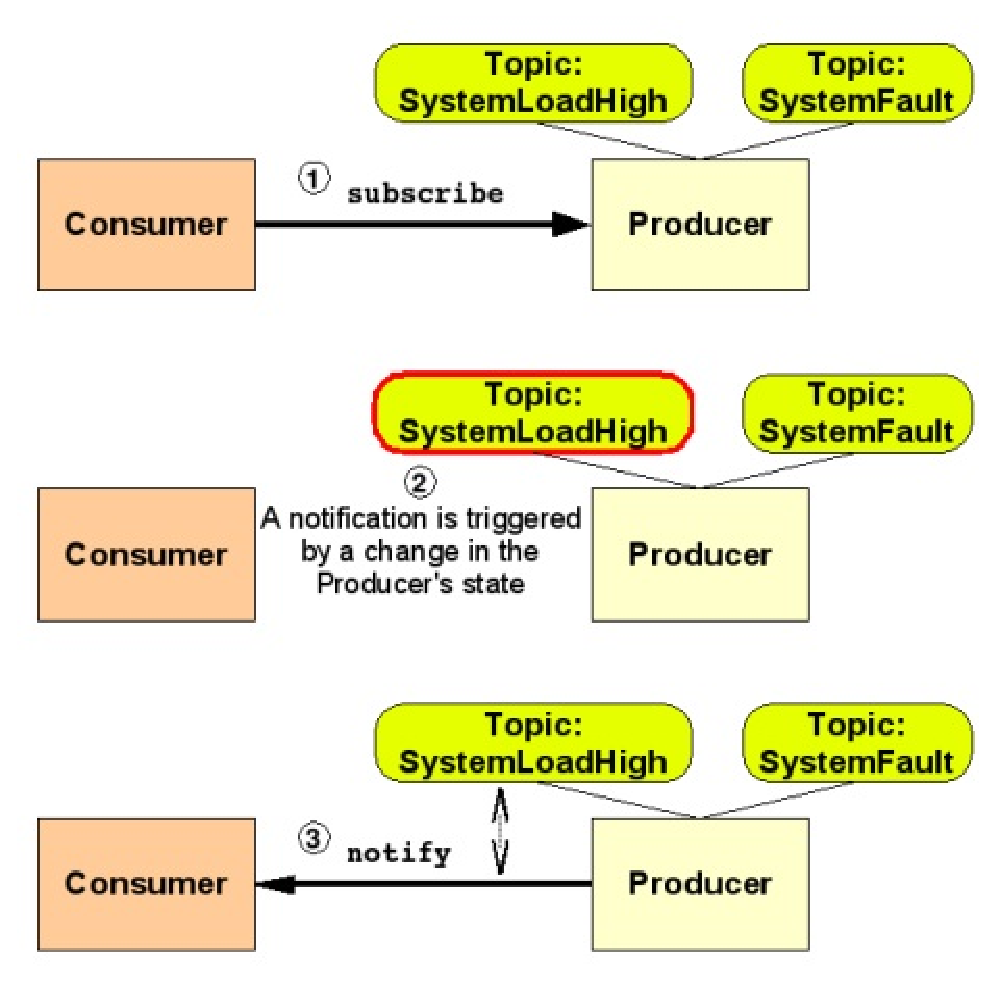
\includegraphics[scale=0.45]{Figures/12}
     \caption{Ejemplo de uso de WS-Notification sin broker.}
  \label{12}
\end{figure}
 
Este caso muestra un ejemplo de interacci�n entre un consumidor y un productor de notificaciones, en el caso de que el suscriptor y el consumidor sean la misma entidad. El sistema es simple ya que tenemos un consumidor y un productor que publica 2 topics: SystemLoadHigh y SystemFault. Los pasos necesarios son: 

\begin{enumerate}
\item En primer lugar, el consumidor se suscribe al topic SystemLoadHigh, por lo que internamente se crea un \emph{Subscription resource} con la informaci�n de la suscripci�n. El productor debe implementar un m�todo \emph{Subscribe} y el consumidor un m�todo \emph{Notify}.  
\item Despu�s, el productor debe enviar una notificaci�n cuando el sistema sobrepase una determinada carga de trabajo. Por ejemplo, nuestro sistema enviar� notificaciones cuando la carga de trabajo sea mayor de 50\%.
\item Por �ltimo, el productor env�a la notificaci�n invocando la operaci�n \emph{Notify} en el consumidor.
\end{enumerate}
   
Un ejemplo de mensaje \emph{Notify} es:
 
\lstset{language=XML, numbersep=5pt, frame=single}
\begin{lstlisting}
...
<wsnt:Notify>
    <wsntw:NotificationMessage>
     <wsnt:Topic Dialect= xsd:anyURI >
       {any}
     </wsnt:Topic>
     <wsnt:ProducerReference>?
      wsa:EndpointReference
     </wsnt:ProducerReference>
     <wsnt:Message>xsd:any</wsnt:Message>
    <wsnt:NotificationMessage>+
</wsnt:Notify>
...
\end{lstlisting}

Como podemos observar el mensaje \emph{Notify} contiene uno o varios mensajes de notificaci�n (\emph{NotificationMessages}). Los campos dentro de �stos son: 

\begin{itemize}
\item Topic: La informaci�n del topic que se env�a.
\item Dialect: El dialecto usado para expresar el topic anterior, es decir, el lenguaje utilizado para expresarlo.
\item ProducerReference: Direcci�n del productor.
\item Message: Una copia de la carga �til (payload) del mensaje actual.
\end{itemize}

A continuaci�n, se muestra el mensaje que manda el suscriptor para registrar su inter�s en uno o m�s topics:


\lstset{language=XML, numbersep=5pt, frame=single}
\begin{lstlisting}
...
<wsnt:Subscribe>
  <wsnt:ConsumerReference>
    wsa:endpointReference
  </wsnt: ConsumerReference>
  <wsnt:TopicExpression Dialect = xsd:anyURI >
    {any}
  </wsnt:TopicExpression>
  <wsnt:UseNotify>xsd:boolean</wsnt:UseNotify>?
  <wsnt:Precondition>wsrp:QueryExpression</Precondition>?
  <wsnt:Selector>wsrp:QueryExpression</wsnt:Selector>?
  <wsnt:SubscriptionPolicy>{any}</wsnt:SubscriptionPolicy>?
  <wsnt:InitialTerminationTime>
    xsd:dateTime
  </wsnt:InitialTerminationTime>?
</wsnt:Subscribe>

...
\end{lstlisting}


Los conceptos importantes en este mensaje son \emph{UseNotify} que se utiliza para decidir si el mensaje de notificaci�n sigue el formalismo WS-Notification o se manda sin formato, \emph{Precondition} que es la condici�n que genera mensajes de notificaci�n, es decir, si se cumple esta condici�n se generan mensajes, pero debe cumplirse tambi�n la condici�n \emph{selector} para enviarlos a los destinatarios que es la que se usa para decidir si se transmiten o no los mensajes generados. Adem�s, \emph{SubscriptionPolicy} se podr�a utilizar para controlar el ratio de env�o de mensajes(por ejemplo, no m�s de 3 por segundo) y \emph{InitialTerminationTime} contiene una sugerencia del tiempo de vida de la suscripci�n. WSRF tambi�n incluye mensajes para detener la suscripci�n, reanudarla o para que un servicio que acaba de unirse a una suscripci�n pueda obtener un historial de notificaciones sobre un determinado topic.



\subsection{WS-BrokeredNotification}

Un \emph{NotificationBroker} es un intermediario que, entre otras cosas, permite el env�o de mensajes entre uno o varios \emph{Publishers} y uno o varios \emph{NotificationConsumers}. La misi�n del \emph{Publisher} es observar ciertas situaciones y crear mensajes de notificaci�n para informar de esas situaciones, mientras que el broker es el encargado de distribuir estos mensajes. \\

En este caso, se pueden dar tres relaciones entre las partes: \emph{simple publishing}, \emph{composable publishing} y \emph{demand-based publishing}. En el primer caso, el \emph{Publisher} es el encargado de observar las situaciones y notificarlas al broker que ser� el encargado de transmitirlas a los interesados. En el segundo caso, el papel del \emph{Publisher} lo realizar� una entidad que implementa una serie de servicios especificados en WS-Notification (NotificationProducer). En este caso, el mensaje de notificaci�n puede llegar a otros consumidores que estuviesen suscritos al productor. En ambos casos, el broker puede pedir al \emph{Publisher} que se registre para poder publicar mensajes sobre un topic determinado. El �ltimo enfoque (\emph{demand-based publishing}) requiere que el \emph{Publisher} sea un \emph{NotificationProducer} y, as�, acepte mensajes de suscripci�n. El objetivo es reducir el n�mero de mensajes de notificaci�n haciendo que �stos solo se manden cuando se soliciten expresamente.





\subsection{Formal models of concurrency}\label{formalmodels}





\section{Summary}\label{sumArt}
\markright{~\ref{sumArt} Summary}



%\chapter[Estado del Arte]{Estado del Arte}

En este cap�tulo se presenta el estado del arte en el campo de la especificaci�n, formalizaci�n y verificaci�n de servicios web, as� como los formalismos y herramientas necesarias para la comprensi�n y elaboraci�n de una futura tesis doctoral. El objetivo es mostrar al lector unas nociones b�sicas en formalizaci�n y servicios web que le facilitar�n la tarea de comprensi�n de la presente memoria.

\section{Introducci�n/Motivaci�n}

A lo largo de la historia de la computaci�n, los ingenieros han usado diferentes m�todos formales para mejorar la calidad del hardware y software. Estos sistemas con el incesante avance tecnol�gico en t�cnicas de integraci�n y metodolog�as de programaci�n crecer�n inevitablemente en escalabilidad y complejidad. Debido a esta complejidad, la probabilidad de error es mayor y, adem�s, alguno de estos errores pueden ocasionar incalculables p�rdidas econ�micas, de tiempo o, incluso, la p�rdida de vidas humanas. Por tanto, el principal objetivo de los ingenieros es facilitar a los desarrolladores la tarea de construir sistemas que tengan un �nfimo ratio de errores y que entren dentro de los m�rgenes comerciales de las empresas. Sin embargo, este tarea no es trivial porque necesitamos asegurar la correcci�n de las especificaciones y necesitamos proporcionar t�cnicas que ayuden a la detecci�n de errores y a la verificaci�n de los modelos desarrollados. Una de las v�as que los ingenieros han venido utilizando para conseguir este objetivo, como se ha comentado anteriormente, es la utilizaci�n de t�cnicas formales, que pueden definirse como el conjunto de procedimientos y herramientas basados en lenguajes matem�ticos que aseguran pr�cticamente la correcci�n de un sistema \cite{Clarke96} porque aumentan el nivel de conocimiento de un sistema, revelando inconsistencias y ambig�edades que no podr�an detectarse con otras t�cnicas, es decir, los m�todos formales ofrecen un mayor grado de refinamiento del modelo que otros m�todos. \\

\begin{figure}
\begin{center}
  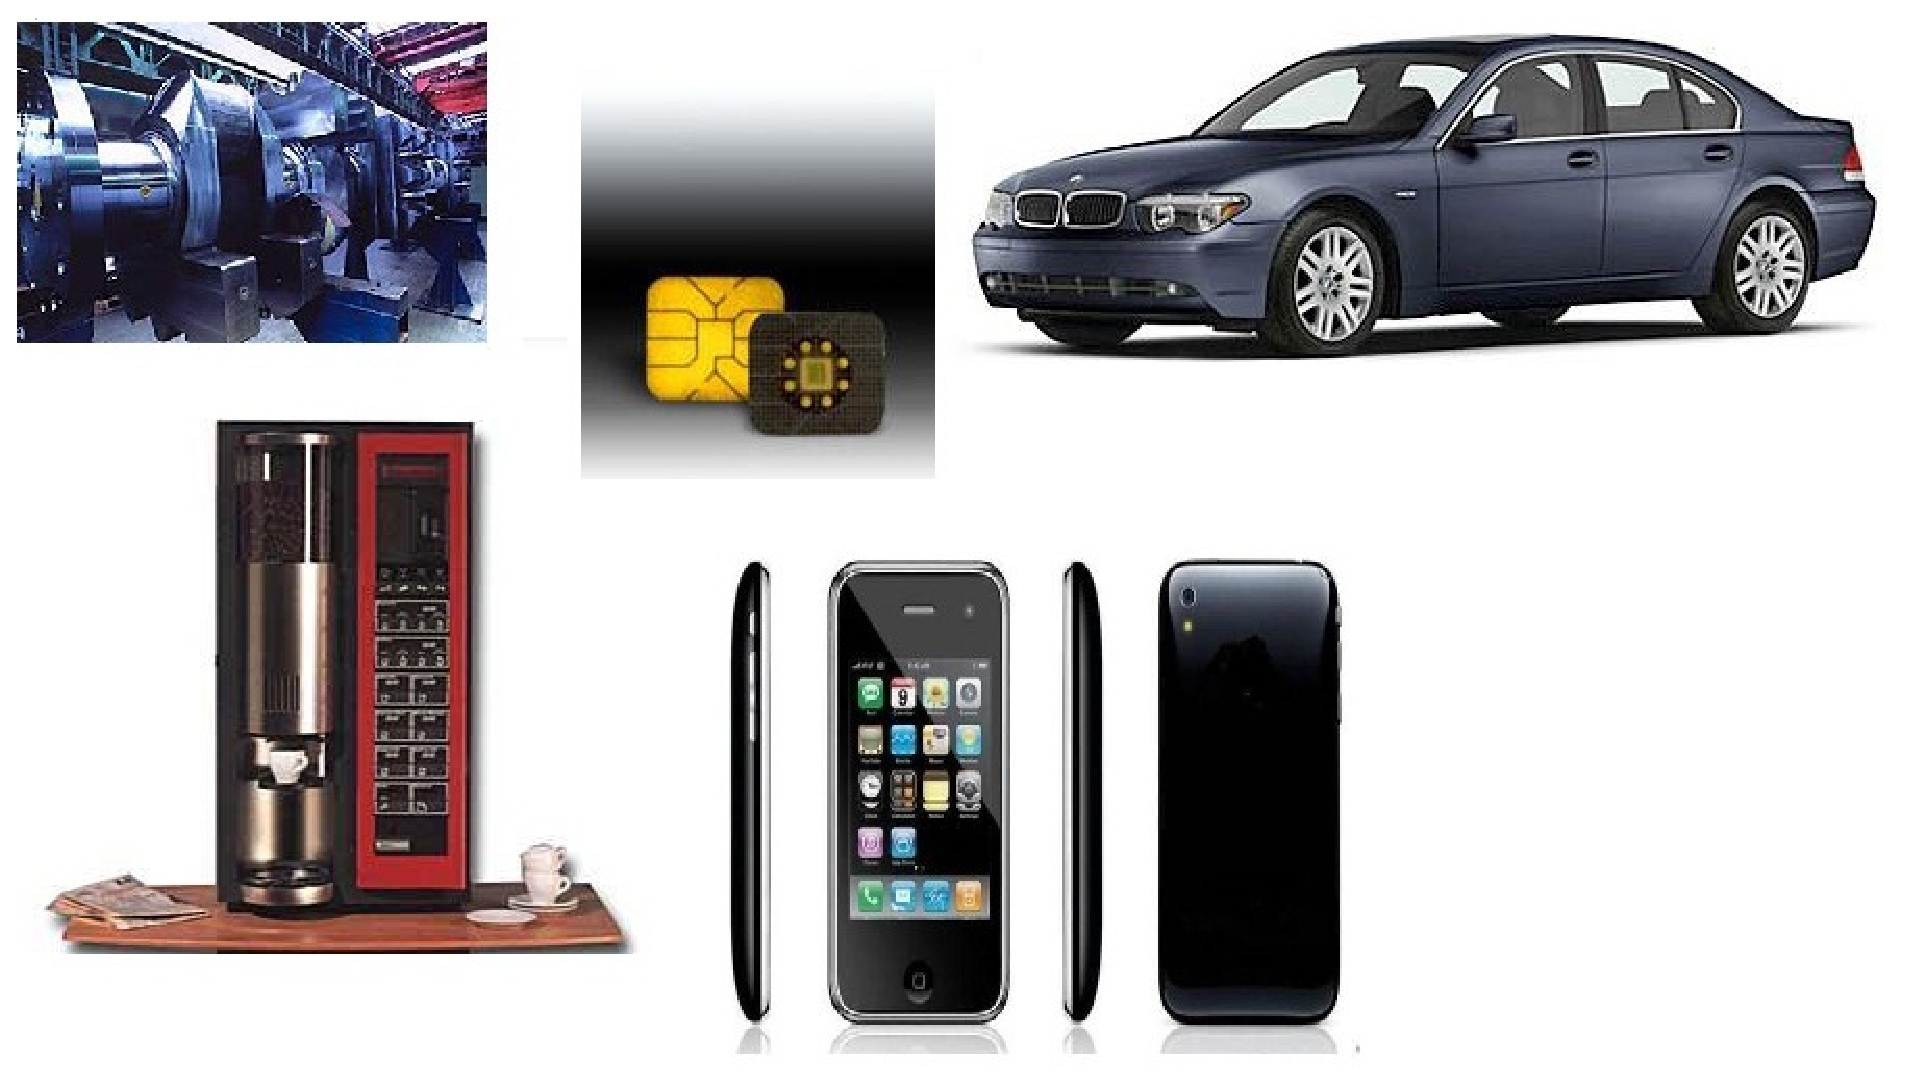
\includegraphics[scale=0.5, width =\columnwidth]{Figures/usos}
\end{center}
  \caption{Ejemplos de sistemas donde se usa la formalizaci�n.}
  \label{uso}
\end{figure}

En el pasado, el uso de t�cnicas formales en la pr�ctica parec�a no tener esperanzas porque las notaciones utilizadas eran demasiado complicadas para los no iniciados en la materia, las t�cnicas no permit�an que el sistema fuese escalable y las herramientas existentes eran demasiado dif�ciles de manejar o, incluso, no exist�an herramientas que modelasen una determinada t�cnica o formalismo. Adem�s, los casos de estudio que exist�an no convenc�an a los desarrolladores sobre la utilidad de la formalizaci�n. Sin embargo, a principios de los a�os 90, se empez� a vislumbrar un nuevo camino en este �rea. Para la especificaci�n de software, la industria empez� a utilizar el lenguaje Z \cite{Abrial80} para obtener especificaciones m�s rigurosas. Para la verificaci�n del hardware, las principales empresas del sector como Intel o AMD utilizan t�cnicas como el \emph{model checking} o \emph{theorem proving}  como complemento a las pruebas realizadas en los simuladores. En ambas �reas, tanto investigadores como desarrolladores est�n describiendo casos de estudio de mayor tama�o, lo que est� beneficiando a que otros desarrolladores est�n plante�ndose la posibilidad de implantar el uso de t�cnicas formales en sus procesos de desarrollo. En la Figura \ref{uso} podemos ver distintos sistemas donde se utilizan actualmente estas t�cnicas para asegurar el correcto funcionamiento de los mismos. Por ejemplo, las compa��as que fabrican aviones utilizan lenguajes formales para especificar los requisitos de los aparatos y las compa��as automovil�sticas verifican los sistemas m�s cr�ticos, en cuanto a seguridad se refiere, utilizando \emph{model checking}. \\

Las principales ventajas de utilizar t�cnicas formales son:

\begin{itemize}
\item El uso de las matem�ticas como base dota a este enfoque de cierto rigor.
\item Identifica la ambig�edad y las inconsistencias.
\item Facilita la construcci�n de sistemas consistentes y libres de \emph{deadlocks}.
\item Otorga confianza al cliente del sistema.
\item Existen multitud de herramientas que dan soporte a las distintas t�cnicas.
\item Encuentra fallos en etapas tempranas que ahorran mucho dinero.
\end{itemize} 

\newpage

Las principales desventajas (o creencias) que ralentizan el avance de este �rea son:

\begin{itemize}
\item Se cree que el uso de formalismos ralentiza el desarrollo.
\item Muchos desarrolladores piensan que es dif�cil trabajar con especificaciones formales.
\item No garantiza la correcci�n del c�digo implementado (s�lo la del modelo
en que se basa).
\item El aumento de la complejidad del sistema provoca un aumento exponencial
de la complejidad de la verificaci�n.
\end{itemize}

Una de las partes m�s importante en el desarrollo de un sistema es la especificaci�n de requisitos. En el �rea de la ingenier�a, una especificaci�n puede verse como un documento t�cnico donde se describen las caracter�sticas y servicios necesarios para construir un producto, aunque tambi�n puede incluir informaci�n sobre etapas posteriores como la verificaci�n, validaci�n, etc., por tanto, si queremos desarrollar sistemas correctos y de calidad debemos dedicar el tiempo necesario a la especificaci�n. De todos modos, realizar la especificaci�n no garantiza la ausencia de errores porque la presencia de fallos es una caracter�stica intr�nseca de los sistemas. En este sentido, el simple hecho de escribir el documento ayuda a los ingenieros a encontrar errores en fases tempranas del desarrollo ahorrando mucho dinero y tiempo al proyecto como puede verse en la Figura \ref{coste}. 

\begin{figure}
\begin{center}
  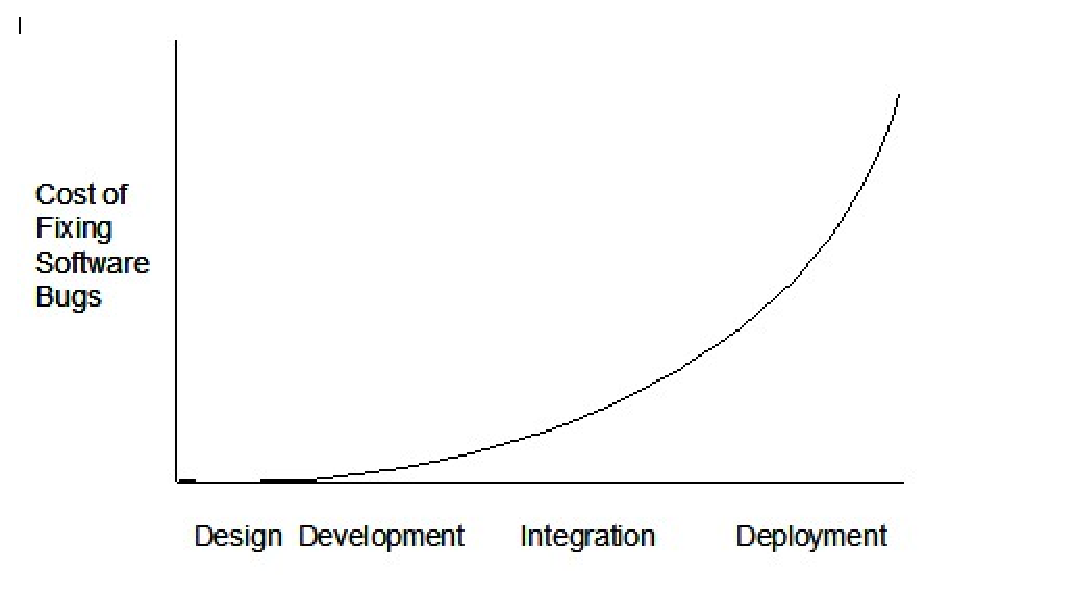
\includegraphics[scale=0.5, width =\columnwidth]{Figures/coste}
\end{center}
  \caption{Evoluci�n del coste de reparaci�n de un fallo.}
  \label{coste}
\end{figure}

\newpage

 
Otra fase del desarrollo donde se utilizan formalismos es en la etapa de \emph{Verificaci�n}. Se puede definir \emph{Verificaci�n} como la etapa donde se comprueba que el producto fabricado cumple con la especificaci�n de requisitos realizada previamente, es decir, en el caso de la inform�tica, que nuestro sistema cumple las propiedades que se describen en la especificaci�n. El objetivo de esta tarea puede resumirse en una de las frases m�s celebres de uno de los padres de los m�todos formales: \\
\begin{center}
\emph{``La verificaci�n de un programa s�lo muestra la presencia de errores, pero nunca garantiza la ausencia de los mismos''}
\end{center}
\vspace{-0.9cm}
\begin{flushright}
Edsger Wybe Dijkstra 
\end{flushright} 

En el ciclo de vida cl�sico, las fases de verificaci�n y validaci�n se realizan despu�s de la fase de implementaci�n, pero, como hemos visto en la Figura \ref{coste}, es necesario detectar estos errores en las fases tempranas del desarrollo. Como es de esperar, es pr�cticamente imposible verificar un sistema completo, por lo que el objetivo de los m�todos formales y de este trabajo de investigaci�n es comprobar si se cumplen ciertas propiedades en el modelo. Las propiedades de inter�s que es necesario verificar estar�n relacionadas con los problemas cl�sicos de concurrencia (\emph{deadlock, exclusi�n mutua, \ldots}), as� como algunos aspectos relacionados directamente con el sistema que se est� construyendo como puede ser comprobar si se cumplen ciertas restricciones temporales. Por ejemplo, en un sistema bancario es necesario verificar si las transacciones cumplen los tiempos estipulados para su realizaci�n, ya que si exceden estas restricciones podr�an ocasionarse problemas de seguridad en el sistema, lo que har�a perder mucho dinero al banco en cuesti�n. Otro ejemplo podr�a ser el sistema de reservas de una aerol�nea, ya que no podemos permitir que un usuario reserve un asiento durante un largo per�odo de tiempo porque podr�a no comprarlo finalmente y evitar que otro lo pudiera adquirir, con el consiguiente perjuicio para la compa��a. \\

Asimismo, se pueden seguir dos v�as para realizar la verificaci�n de un sistema: \emph{Human-directed proof o Automated proof}. El primer caso se utiliza cuando se quiere afianzar el conocimiento sobre el sistema en lugar de asegurar completamente la correcci�n del mismo, por lo que es una persona la que realiza de forma manual la verificaci�n. En la segunda aproximaci�n (\emph{automated proof}) tenemos dos variantes: \emph{automated theorem proving y model checking}. El \emph{automated theorem proving} consiste en que un programa trata de producir una prueba formal de un sistema desde el principio, dando una descripci�n del mismo, un conjunto de axiomas l�gicos y una serie de reglas de inferencia. Model checking \cite{Clarke99} es una t�cnica autom�tica para verificar sistemas reactivos de estados finitos. En esta aproximaci�n, la especificaci�n est� expresada en l�gica proposicional temporal, normalmente LTL \cite{Pnueli77} o CTL \cite{Henzinger94} o algunas de sus variantes, y el sistema se representa como un grafo de transiciones entre estados conocido como \emph{aut�mata}. En esta t�cnica debe utilizarse un eficiente m�todo de b�squeda para determinar si el aut�mata satisface la especificaci�n. El \emph{model checking} tiene numerosas ventajas sobre \emph{automated theorem proving}, pero la m�s importante es que el proceso tiene m�s partes que se pueden automatizar, por lo que la fase de prueba (\emph{testing}) dentro del ciclo de vida del sistema es m�s r�pida. Normalmente, el cliente s�lo pone a disposici�n del ingeniero una representaci�n a alto nivel del sistema (generalmente, en lenguaje natural) y la especificaci�n del mismo, tambi�n en lenguaje natural. As�, cualquier \emph{model checker} (Spin \cite{Holz04}, UPPAAL \cite{Larsen97}, etc.) termina el proceso con una respuesta afirmativa si el modelo propuesto satisface la especificaci�n o proporciona un contraejemplo para localizar d�nde se ha producido el error.
 

\section{Model Checking para Sistemas de Tiempo Real}

Los sistemas donde el tiempo juega un papel crucial para su funcionamiento y evoluci�n son conocidos como ``Sistemas de Tiempo Real (Real-Time Systems)''. Este tipo de sistemas son el n�cleo que controla la mayor�a de sistemas industriales, financieros y gubernamentales, donde el tiempo de respuesta determina el grado de correcci�n, la eficiencia, la satisfacci�n del usuario y otras variables de calidad, por lo que su correcto funcionamiento es vital para evitar errores que pueden ocasionar grandes p�rdidas. Sin embargo, dentro de estos sistemas existe otro tipo, donde las restricciones temporales juegan un papel realmente crucial, conocido como ``strong time restrictions''. En este entorno es necesario verificar completamente que el sistema tiene un ratio de error �nfimo porque un simple fallo podr�a ocasionar que el sistema dejara de funcionar. Otra informaci�n �til es la probabilidad de fallo cuando �ste no se puede eliminar. Esta medida sirve para dar confianza a los clientes, ya que un sistema con baja probabilidad de error aumenta el grado de satisfacci�n y confianza en el mismo. Esta informaci�n permite medir la necesidad de redise�ar el sistema o de mantenerlo en funcionamiento. En este caso, el fallo se debe a un factor externo que el sistema no puede manejar, como, por ejemplo, el tiempo, las leyes f�sicas o desastres naturales. Todos estos factores tienen en com�n que su aparici�n es incontrolable, pero es posible predecir su aparici�n con una razonable probabilidad. As�, existen sistemas donde la combinaci�n de ambas caracter�sticas, ``tiempo'' y ``probabilidad'', determinan las caracter�sticas principales del mismo, por lo que las t�cnicas de verificaci�n no s�lo tienen que tener en cuenta las restricciones temporales sino que deben considerar la probabilidad de que ocurran sucesos inesperados.      


\section[UPPAAL]{UPPAAL - Una herramienta para la verificaci�n autom�tica de Sistemas de Tiempo Real}

UPPAAL es una herramienta para la verificaci�n autom�tica de dos propiedades cruciales en los sistemas inform�ticos: \emph{safety} y \emph{liveness}, es decir, debemos asegurar que nuestro sistema es consistente (seguro) ante posible ataques o fallos y que permanecer� funcionando ante estos contratiempos \cite{Alur94}. El motor de UPPAAL transforma una clase de sistemas lineales h�bridos en redes de aut�matas temporizados e implementa t�cnicas basadas en la resoluci�n de restricciones. UPPAAL tambi�n ofrece valiosa informaci�n de diagn�stico en el caso de que la verificaci�n falle. Las siguientes secciones se centrar�n en aspectos formales de la herramienta.\\

La versi�n actual de la herramienta puede encontrarse en \textsf{http://www.uppaal.com}. A pesar de que fue desarrollada en 1995, actualmente cuenta con muchas caracter�sticas (probabilidades, costes, energ�a, etc.), gracias a la labor de investigaci�n realizada durante estos a�os. Debido a este alto grado de madurez y a la facilidad para conseguir informaci�n por las colaboraciones del grupo ReTiCS con la universidad de Aalborg, se ha seleccionado esta herramienta en lugar de otras. 




\section{Services Oriented Computing (SOC)}

Aunque la Web fue inicialmente concebida para el uso exclusivo del ser humano, muchos expertos consideran que tiene que evolucionar (probablemente a trav�s del dise�o y construcci�n de servicios modulares) para soportar mejor la automatizaci�n de muchas tareas. El concepto de \emph{servicio} proporciona un mayor nivel de abstracci�n para organizar las aplicaciones a gran escala y construir entornos m�s abiertos, ayudando a desarrollar aplicaciones con mejor productividad y calidad que las que podr�amos fabricar con otros enfoques. Puesto que los servicios son s�lo un medio para la construcci�n de aplicaciones distribuidas, no podemos hablar de ellos sin hablar de las aplicaciones basadas en servicios, en concreto, c�mo se construyen y c�mo los servicios deben funcionar conjuntamente dentro de ellas. La Figura \ref{arq} muestra un ejemplo de arquitectura basada en servicios, donde como puede observarse hay tres partes principales: un proveedor, un consumidor y un registro. 

\begin{figure}
\begin{center}
  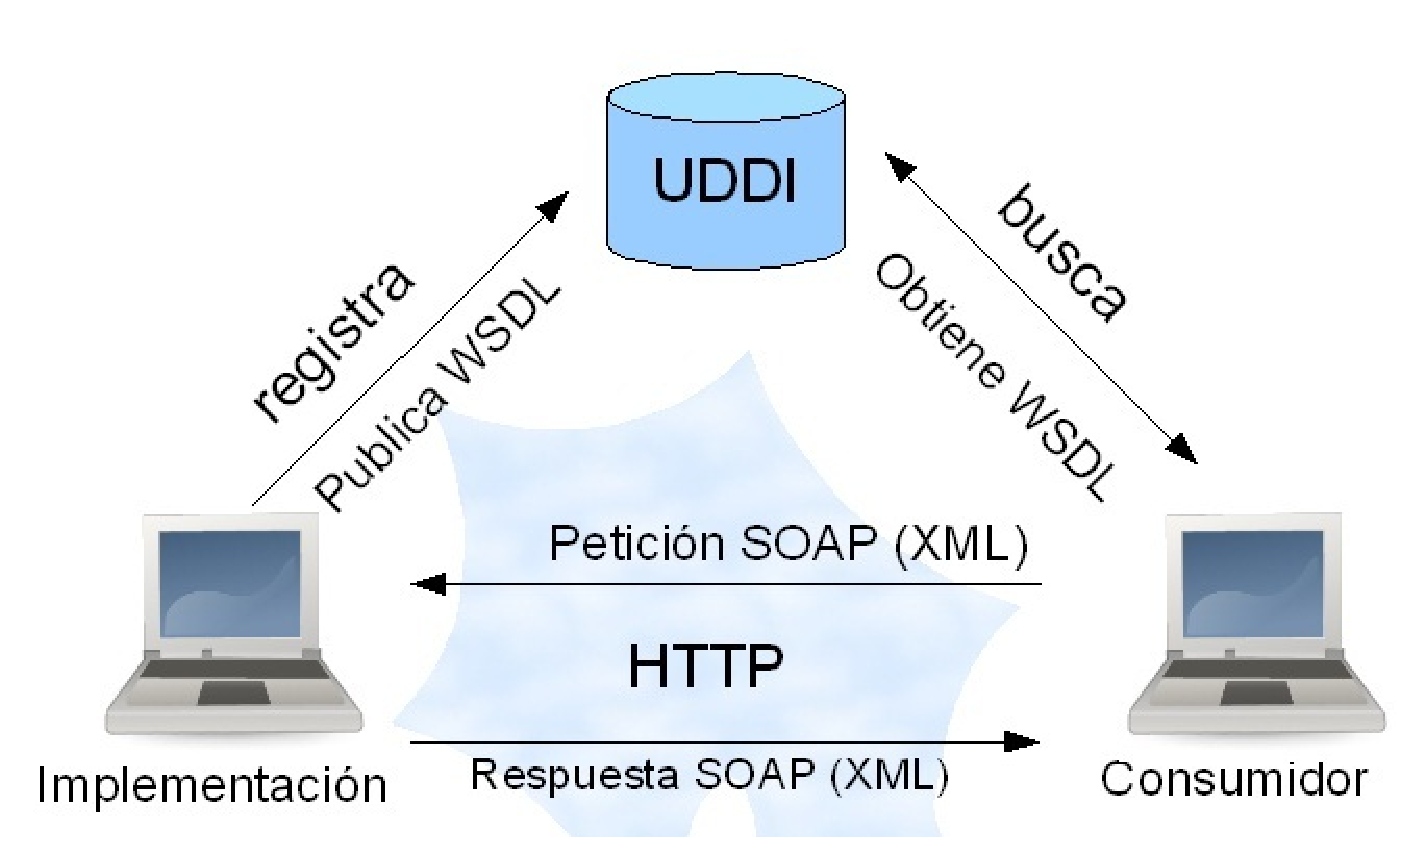
\includegraphics[width =\columnwidth]{Figures/arquitecturaWS}
\end{center}
  \caption{Arquitectura cliente-servidor para servicios web.}
  \label{arq}
\end{figure}

La funci�n de los proveedores es publicar o anunciar los servicios que ofrece en los registros, donde los consumidores pueden encontrarlos y, posteriormente, invocarlos. Los actuales est�ndares que sustentan las interacciones entre servicios web proporcionan una base s�lida para la arquitectura orientada a servicios, pero no soportan servicios esenciales para su funcionamiento completo. De hecho, aunque los servicios web proporcionan una fuente de ejemplos pr�cticos, son innecesariamente limitados. La arquitectura web es un marco que puede ser reforzado con representaciones m�s poderosas y t�cnicas tomadas de otros enfoques. Muchos profesionales utilizan estas representaciones, a pesar de que se omiten en la mayor�a de los libros. 

\section{Cloud Computing/Grid Computing}
Gracias a la r�pida evoluci�n que ha tenido la sociedad, servicios b�sicos para el desarrollo de la vida cotidiana son com�nmente suministrados a los ciudadanos, de tal manera, que cualquier persona puede tener acceso inmediato a ellos de forma f�cil. Hoy en d�a, estos servicios, conocidos en el mundo anglosaj�n como ``utility services'', engloban el suministro de agua, electricidad, gas y tel�fono, pero en los �ltimos tiempos est� cobrando fuerza una vieja idea que se intent� llevar a cabo sin �xito a finales de los a�os 60 y principios de los 70, el ``Utility Computing''. Este nuevo paradigma de computaci�n es normalmente confundido con Cloud o Grid Computing, pero hay ciertos matices que los diferencian. ``Utility Computing'' se puede entender como el modelo de negocio que subyace en una infraestructura Cloud o Grid, es decir, puede ser entendido como el medio de cobro de servicios computacionales similar al que se hace con la electricidad, por lo que el usuario pagar� s�lo por su consumo, mientras que los costes asociados a la producci�n y distribuci�n de potencia de c�mputo ser�n sufragados por las compa��as suministradoras. As�, las peque�as y medianas empresas podr�an competir en igualdad de condiciones con las grandes empresas, ya que no ser�a necesario hacer una gran inversi�n en datacenters para poder ofrecer un determinado servicio y se fomentar�a la creaci�n de empresas, ya que estos datacenters suponen una fuerte inversi�n inicial que muchos emprendedores no pueden acometer. Adem�s, el usuario final de las aplicaciones, servicios o infraestructuras tambi�n se beneficiar�a porque al reducir costes de producci�n se reduce el precio de los productos. Por seguir con el s�mil de la energ�a, podemos ver el cloud computing como una gran central generadora de energ�a que da suministro a millones de usuarios y que evita que dichos usuarios tengan que tener su propia central en casa para poder encender sus aparatos el�ctricos, mientras que el ``utility computing'' es la forma de tarificar el gasto de los usuarios o, de una forma m�s abstracta, podemos verlo como el contador que muestra el consumo energ�tico. Al igual que pasa con el software, los protocolos o cualquier paradigma relacionado con la inform�tica, Cloud Computing debe atravesar una serie de etapas para poder comprobar si toda esta publicidad que le est�n dando las empresas sirve de veras para ahorrar costes y favorecer la competitividad o solo es m�s una forma de aumentar ingresos o, en el caso de la investigaci�n, obtener nuevos fondos. En este sentido, algunos autores consideran que Cloud Computing no es mas que una nueva forma de nombrar lo que toda la vida se ha llamado Grid o Web Services y que realmente no supone ning�n avance en el campo de la inform�tica. Este art�culo tratar� de presentar m�s ampliamente la arquitectura y conceptos para comprender un sistema de computaci�n basado en la nube y mostrar� las diferencias entre dos enfoques cl�sicos de computaci�n (Grid y Web Services) y Cloud. Finalmente, se propondr� una serie de ideas que pueden llegar a convertirse en trabajos de investigaci�n en un futuro.         

\section{Introducci�n}

En 1943, el presidente de IBM, Thomas J. Watson, predijo:

\begin{center}
``I think there is a world market for about five computers''
\end{center}

Esta frase, tan comentada en el mundo de la inform�tica en los �ltimos tiempos, ha pasado de ser una predicci�n con poco fundamento a ser una realidad en la actualidad.\\

Cloud Computing, el viejo sue�o de ofrecer servicios de computaci�n como utilidad, tiene el potencial de transformar gran parte de la industr�a inform�tica, haciendo el software m�s atractivo al ofrecerlo como servicio y moldeando la forma en que se dise�a y compra el hardware. Con este nuevo enfoque, cualquier emprendedor con buenas ideas para ofrecer servicios a trav�s de Internet no necesitar� realizar grandes inversiones en equipamiento para llevar a cabo su proyecto ni necesitar� contratar inicialmente mucho personal que gestione y mantenga dicho equipamiento. Adem�s, no tiene que realizar complicados estudios previos para calcular el n�mero de usuarios potenciales y evitar, as�, unos de los principales quebraderos de cabeza de los jefes de proyecto: el sobre-aprovisionamiento o el infra-aprovisionamiento. Estos dos conceptos junto con la elasticidad de recursos pueden ser considerados como claves en computaci�n en la nube, ya que el objetivo de reducir costes es directamente proporcional a la correcta estimaci�n de recursos en ``tiempo real'' y esta correcta estimaci�n s�lo se puede proporcionar si el sistema cumple la propiedad de elasticidad, es decir, que en un intervalo de tiempo relativamente corto aumentas y disminuyes los recursos dedicados a una tarea con un coste econ�mico bajo. Este enfoque puede hacer que, a primera vista, no se perciba la posibilidad de utilizar m�todos formales con este tipo de sistemas, puesto que normalmente se utilizan t�cnicas formales en el dise�o de sistemas con tiempos de respuesta cr�ticos como sistemas de navegaci�n de un avi�n, transporte de materiales peligrosos, etc. De esta manera, se hace inviable el uso de la computaci�n en la nube cuando se exijan tiempos de respuesta muy bajos, ya que, por ejemplo, un sistema de navegaci�n de un avi�n no puede esperar varios minutos a que se le asignen nuevos recursos para tomar una decisi�n. Sin embargo, si que hay otro tipo de sistemas en los que los m�todos formales y el cloud computing pueden converger, los sistemas de alta disponibilidad.\\

As�, utilizando t�cnicas formales se pueden dise�ar este tipo de sistemas y verificar la ausencia de fallos en su construcci�n. Por ejemplo, una tienda de venta online podr�a pasar de tener cientos de usuarios simult�neamente a miles de ellos en periodos como las vacaciones de Navidad, de manera que necesitar�a mucha mayor potencia de computaci�n si quiere satisfacer a todos los clientes y no perder ingresos ni nuevos clientes por no poder atender esa demanda. Para satisfacer esta necesidad, har�a un estudio preliminar de cuantas visitas como m�ximo puede tener en ese per�odo y comprar�a los datacenters necesarios para no tener problemas de congesti�n, lo que supone una inversi�n grande en infraestructura por parte de la compa��a, sin embargo, una vez acaba la campa�a navide�a la demanda de usuarios vuelve a ser de unos cientos y la empresa se encuentra con que tiene una potencia de c�mputo que no va a necesitar y, por tanto, no est� amortizando econ�micamente la inversi�n realizada. En este sentido, si la compa��a en lugar de comprar los datacenters hubiese comprado capacidad de c�mputo a un proveedor entonces habr�a amortizado en mayor medida el dinero invertido y no tendr�a m�quinas en sus oficinas que ocupan bastante espacio y que tienen unos niveles de carga de trabajo muy bajos.  \\


Cloud Computing se refiere tanto a las aplicaciones que se ofrecen como servicios a trav�s de Internet como al hardware y software que est� presente en los datacenters que proveen dichos servicios. Estos servicios se han referido normalmente como Software as a Service (SaaS). El datacenter en s� es lo que se considera la nube (o cloud). Desde el punto de vista del hardware, hay tres aspectos novedosos en Cloud Computing: 

\begin{enumerate}
\item La ilusi�n de tener recursos ilimitados bajo demanda eliminando a los usuarios la necesidad de aprovisionarse antes de acometer una tarea.
\item La eliminaci�n de la inversi�n inicial en equipamiento permitiendo a las compa��as empezar con pocos recursos e ir aument�ndolos cuando las necesidades aumenten.
\item La posibilidad de pagar por el uso de recursos de computaci�n a corto plazo seg�n se necesiten (por ejemplo, procesadores por hora o capacidad de almacenamiento de datos por d�a) y poder liberarlos cuando no sean necesarios. 
\end{enumerate}

Cloud Computing podr�a tener el mismo impacto en la producci�n de software que el que tuvieron las fundiciones de metal en la industr�a del hardware. En principio, las compa��as fabricantes de hardware necesitaban tener sus propias instalaciones donde fabricar los componentes que compon�an sus productos, lo que les supon�a un gran esfuerzo econ�mico para construir y operar estas instalaciones y, por consiguiente, hac�a que el precio de los equipos se doblase en cada nueva generaci�n. Sin embargo, la aparici�n de compa��as que fabricasen componentes favoreci� que empresas m�s peque�as pudiesen entrar en el mercado del hardware, copado hasta aquel entonces por Intel o Samsung, que eran las �nicas que pod�an hacer frente a este gran esfuerzo econ�mico. De manera similar, la computaci�n en la nube podr�a jugar el papel que hicieron las fundiciones, favoreciendo la competencia y evitando monopolios de grandes empresas. \\

Debido a que muchas empresas usan servicios software como base para su modelo de negocio, se presentan, a continuaci�n, los actores que formar�n parte de este escenario. Los \emph{Services Providers}(SPs) hacen accesibles los servicios a los \emph{Service Users} por medio de interfaces que se comunican a trav�s de Internet. Dado que uno de los objetivos de la nube es externalizar la provisi�n de servicios, se necesita la aparici�n de otro actor que ofrezca esta infraestructura como ``servicio'' llamado \emph{Infrastructure Provider}, migrando los recursos desde los SPs al IPs y, as�, los SPs pueden ganar flexibilidad y reducir costes como se puede ver en la figura \ref{act}. 

\begin{figure}[bth]
  \center
    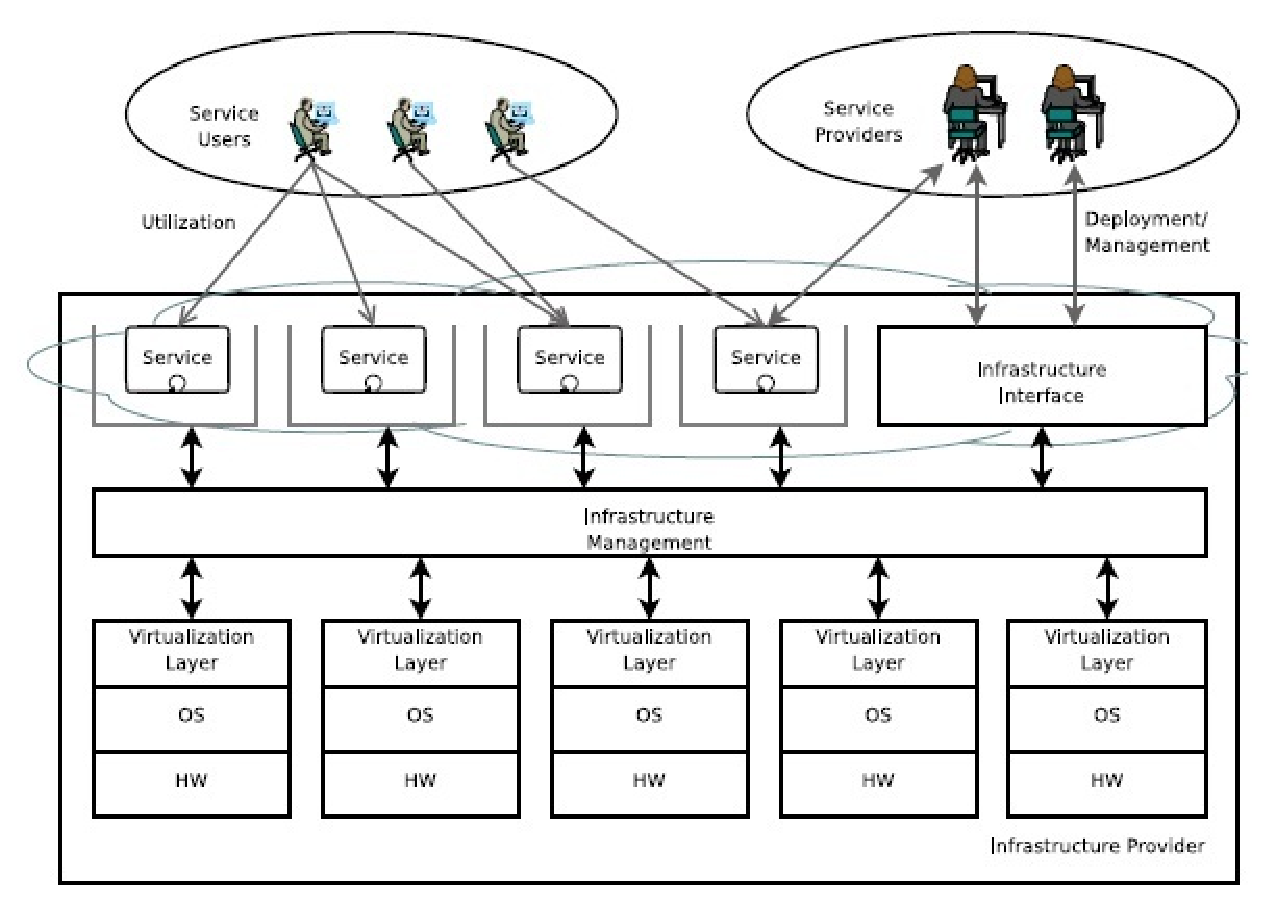
\includegraphics[scale=0.5]{Figures/actores}
  \caption{Actores en un sistema en la nube.}
  \label{act}
\end{figure}

\section{Comparaci�n entre servicios web y Grid computing/Cloud computing}

Como es sabido, nuestro grupo de investigaci�n ha centrado su investigaci�n en el desarrollo de una metodolog�a que permita construir y verificar sistemas con restricciones temporales mediante el uso de t�cnicas formales. En los �ltimos a�os, se ha aplicado esta metodolog�a en el �rea de los servicios web, m�s concretamente, en que estos servicios cumplan la tarea que se les encomienda y que se coordinen autom�ticamente para conseguir llevar a cabo un trabajo m�s general. El problema que est�n teniendo los servicios web es que como tuvieron un gran auge hace pocos a�os, muchos grupos de investigaci�n centraron sus estudios en este campo y, por tanto, hay muchos investigadores proponiendo nuevas aproximaciones y �sto ha llevado a que existen ciertas partes como BPEL o WS-CDL que est�n bastante estudiadas. De esta manera, esta surgiendo un sistema donde los m�todos formales pueden jugar un papel muy importante y donde nuestro grupo puede beneficiarse de su amplia experiencia tanto en formalizaci�n como en servicios web, el cloud computing. Este nuevo paradigma, como se ha expuesto anteriormente, est� viviendo su �poca de plenitud en este momento y grandes empresas como Google, IBM, Microsoft han decidido dar un paso al frente y apostar fuertemente por la computaci�n en la nube. Adem�s, muchos gobiernos est�n interesados en migrar sus servicios a la nube para abaratar costes y permitirles escalabilidad cuando les sea necesaria. Por ejemplo, hay que preguntarse si es necesario para la Agencia Tributaria tener grandes centros de datos cuando la demanda de servicios por parte de los ciudadanos s�lo crece en la �poca de la declaraci�n de la renta. Probablemente la respuesta sea afirmativa porque s� necesita almacenar todos esos datos y dar cierta confianza de que tus datos fiscales no van a caer en manos de gente con no muy buenas intenciones, pero toda la necesidad de c�lculo si que se puede externalizar para ahorrar costes en equipamiento o incluso podr�an crear una nube privada entre todos los organismos que colaboren con la agencia p�blica para compartir recursos e informaci�n. En este sentido, este tipo de sistemas donde la seguridad, privacidad y la disponibilidad son un requisito innegociable es donde podemos centrar parte de nuestras investigaciones e intentar mejorar alguno de los componentes de la arquitectura cloud expuesta en el apartado anterior. Por ejemplo, la mayor�a de grupos de investigaci�n desarrollan herramientas, pero la fase de pruebas o no existe o se le dedica poco tiempo. La semana pasada nos reunimos con uno de los grandes investigadores en el campo del Grid/Cloud Computing, Karim Djemame, y nos cont� que el principal problema que ten�a era ese que no sab�an concretamente porque funcionaba bien su herramienta y que estaba bastante interesado en la verificaci�n de su herramienta. \\


Por otro lado, a continuaci�n se enumeran algunas diferencias entre servicios web y grid/cloud computing para ver donde es posible aplicar nuestra experiencia en este sistema. En primer lugar, podemos considerar que los servicios web son en s� software que se ofrece como servicio (SaaS), aunque existan ciertas diferencias entre ambos enfoques, por ejemplo, la estandarizaci�n. Por tanto, este software podr�a estar compuesto de un conjunto de servicios, probablemente comunicados a trav�s de Internet, y que se coordinan para realizar una determinada tarea. Hasta el momento, nada nuevo, pero la principal diferencia reside en la virtualizaci�n, ya que los diferentes servicios que ofrece la nube se realizan en m�quinas virtuales en lugar de directamente sobre un servidor como puede ser el caso del servicio web, de manera que la concurrencia en el sistema es mayor. \\

Otra diferencia es la persistencia de los datos. Si queremos coordinar varios servicios web para que realicen sumas la �nica posibilidad de que �stos puedan almacenar el resultado es guard�ndolo en la base de datos, sin embargo, existe una aproximaci�n llamada WSRF (Web Services Resources Framework) que ha sido estandarizada y que resuelve este problema. En este framework cada servicio web lleva asociado un recurso o varios del sistema de manera que puedes interactuar con el servicio y decidir a que recurso acceder. La principal ventaja que tiene es que todos los servicios se definen con WSDL (Web Services Description Language) y que la comunicaci�n, direccionamiento, etc. est� estandarizado, de manera que la colaboraci�n entre sistemas de este tipo es sencilla. Otra ventaja es que el usuario tiene la posibilidad de decidir con que recursos interact�a. As�, podr�amos a�adir una capa inferior en nuestra metodolog�a que permitiese la definici�n de servicios web con recursos y una vez verificado que el sistema es correcto, desplegar estos servicios web en las m�quinas f�sicas. Este enfoque encajar�a perfectamente con nuestra investigaci�n, ya que utiliza servicios web con recursos y estos recursos tienen restricciones temporales para evitar que un usuario abarque todo el sistema. \\   

Tambi�n, podemos observar que cloud computing podr�a verse como una capa que se colocar�a debajo de los servicios web, ya que se puede utilizar �stos para acceder a los recursos, pero hay que resaltar que la nube no es solo ofrecer software como servicio, sino que tambi�n hay infraestructura y plataforma como servicio, cosa que los servicios web no pueden abarcar. Es decir, una parte del cloud computing (SaaS) puede compararse directamente con los servicios web, pero las otras dos partes no tienen nada que ver, por lo que ser�a como comparar el protocolo TCP/IP con la arquitectura de un PC, aunque es necesario que ambas aproximaciones (servicios web y cloud computing) converjan para el crecimiento de ambos paradigmas, igual que grid computing y servicios web convergieron en WSRF. \\

Por �ltimo, a modo de curiosidad la principal diferencia entre un sistema grid y uno cloud reside en la virtualizaci�n, ya que en grid el usuario no comparte en tiempo real los recursos que tiene asignados, mientras que en cloud es indispensable la virtualizaci�n de recursos para conseguir dar servicio a m�s clientes y conseguir ese ahorro que prometen los proveedores.

\section{Web Services Resource Framework(WSRF)}

La arquitectura que presentan los servicios web ha sido ampliamente aceptada como medio para estructurar las interacciones existentes entre los servicios que forman parte de un sistema distribuido y que colaborar para conseguir un objetivo com�n. En la actualidad, los desarrolladores requieren a los entornos una mayor estandarizaci�n para facilitar interoperatividad adicional entre dichos servicios, pero hasta mediados de 2004 ning�n grupo de investigaci�n o grupo de expertos se hab�a planteado seriamente la idea de proponer un est�ndar para modelar la comunicaci�n entre servicios web que poseen recursos persistentes asociados. As�, en Enero de ese a�o, varios miembros de la organizaci�n \emph{Globus Alliance} y de la multinacional inform�tica IBM definieron, con la ayuda de expertos de empresas como HP, SAP, Akamai, etc., la especificaci�n de los documentos que deber�an producirse en este modelo y la base de una arquitectura inicial. Estos documentos fueron enviados a la organizaci�n encargada de su estandarizaci�n, OASIS, en Marzo de 2004. En un principio, se formaron dos comit�s que se encargar�an del estudio y desarrollo de ciertas partes de este nuevo est�ndar. Por un lado, estaba el \emph{WSRF Technical Committee} que gestionaba cuatro especificaciones: \emph{WS-ResourceProperties, WS-ResourceLifetime, WS-ServiceGroup, y WS-BaseFaults}. Por otro lado, el \emph{WSN Technical Committee} se encargaba de las especificaciones: \emph{WS-BaseNotification, WS-Topics, y WS-BrokeredNotification}. \\

WS-Resource Framework est� inspirado en el trabajo realizado previamente por el \emph{Global Grid Forum's Open Grid Services Infrastructure (OGSI) Working Group} \cite{Foster03}. M�s concretamente, puede ser visto como una sencilla refactorizaci�n de los conceptos e interfaces desarrollados en la especificaci�n \emph{OGSI V1.0}, de manera que explota los recientes desarrollos en el �rea de los servicios web (por ejemplo, WS-Addressing). \\

El objetivo de este trabajo es introducir los conceptos fundamentales para la gesti�n y destrucci�n de servicios web persistentes, es decir, servicios web que llevan asociados recursos donde guardar los estados de los mismos, ya que hasta la aparici�n de esta aproximaci�n, los servicios web eran considerados ``\emph{stateless}'' y, por tanto, no pod�an almacenar temporalmente datos o resultados de sus operaciones de una manera sencilla para el usuario, ya que era necesario almacenarlos en una base de datos ajena al servicio. En este enfoque, es necesario codificar la relaci�n entre el servicio y el recurso en t�rminos de patrones utilizando una serie de tecnolog�as ampliamente estudiadas, como, por ejemplo, el WS-Addressing y, tambi�n, ser� necesario hacer sus propiedades accesibles desde el exterior a trav�s de un interfaz. En este sentido, llamaremos \emph{WS-Resource} a la asociaci�n entre un servicio web y un recurso persistente.  


\subsection{Introducci�n}

WS-Resource Framework \cite{Ban06} es una especificaci�n, desarrollada por OASIS y algunas de las empresas inform�ticas m�s pioneras, cuyo prop�sito es definir un marco gen�rico para el modelado y acceso a recursos asociados a servicios web, as� como las relaciones entre dichos recursos en un entorno Grid/Cloud. Esta aproximaci�n est� compuesta por un conjunto de especificaciones que definen la representaci�n del WS-Resource en los t�rminos que especifican los mensajes intercambiados y los documentos XML relacionados. Asimismo, incluye mecanismos que describen el medio para consultar el estado de un recurso y la descripci�n del servicio, que forman conjuntamente la definici�n de un WS-Resource. Adem�s, definen los pasos necesarios para hacer el estado de un servicio web accesible a trav�s de su interfaz (descrita en WSDL).\\

Normalmente, las interfaces de los servicios web proporcionan al usuario la posibilidad de acceder y manipular el estado del mismo, como, por ejemplo, valores de datos que evolucionan por la interacci�n entre varios servicios. En otras palabras, los intercambios de mensajes que se implementan en el comportamiento de los servicios tienen como objetivo permitir el acceso a estos recursos persistentes. Sin embargo, la noci�n de recursos persistentes que subyace en la implementaci�n de los servicios no es tan evidente en la definici�n de la interfaz \cite{Fost04}. Los mensajes que estos servicios env�an y reciben implican (o animan al programador a inferir) la existencia de un tipo de recurso asociado. Por tanto, es deseable que se definan est�ndares que permitan el descubrimiento, creaci�n, introspecci�n, interacci�n y destrucci�n de dichos recursos y que la forma elegida para llevar a cabo esta misi�n sea lo m�s interoperable posible. Estas observaciones han motivado la aparici�n de la propuesta comentada anteriormente, WS-Resource, para modelar estados en el contexto de los servicios web. Un WS-Resource se define como la composici�n de un servicio web y sus recursos persistentes asociados, esto es, \emph{(i)} expresado como una asociaci�n de un documento XML con un tipo definido con uno o varios \emph{portTypes} (un servicio podr� jugar un determinado rol si implementa todos los \emph{portTypes} que comprenden ese rol) y \emph{(ii)} direccionado y accedido de acuerdo al patr�n del recurso impl�cito, una derivaci�n de las \emph{Endpoint References} del WS-Addressing. Una \emph{Endpoint Reference} estar� compuesta por: Uniform Resource Identifier (URI), par�metros del mensaje que se envi� para solicitar el env�o de la \emph{Endpoint Reference} y datos relativos a la interfaz que se usa. En este intercambio, el identificador del recurso persistente es encapsulado en una \emph{Endpoint Reference} y usado para identificar al recurso en cualquier intercambio de mensajes entre los servicios que formen la coreograf�a. As�, WSRF permite declarar, acceder, monitorizar y destruir WS-Resources mediante mecanismos convencionales, lo que facilita la tarea de gesti�n, ya que no es necesario hacer m�s dif�cil la l�gica de decisi�n del servicio propietario del recurso para procesar los mensajes de gesti�n. Estos mecanismos convencionales componen cinco especificaciones t�cnicas que definen los medios por los cuales:

\begin{itemize}
\item Se destruye un WS-Resource, ya sea de manera s�ncrona con respecto a una petici�n expl�cita de destrucci�n o, a trav�s de un mecanismo basado en tiempos (scheduled). Adem�s, es posible declarar unas caracter�sticas espec�ficas  de los recursos (WS-ResourceProperties) que podr�an ser utilizadas para inspeccionar y monitorizar el tiempo de vida de dicho WS-Resource (WS-ResourceLifetime).
\item  Se definen los tipos de WS-Resource, que est�n compuestos por la interfaz de la descripci�n del servicio web (WSDL) y por un documento XML de propiedades del recurso. Por otro lado, el estado del WS-Resource puede ser consultado y modificado a trav�s del intercambio de mensajes (WS-ResourceProperties)
\item Un Endpoint Reference (WS-Addressing) puede ser renovado cuando su informaci�n de direccionamiento ha caducado o ha dejado de ser v�lida por alg�n error (WS-RenewableReferences).
\item Adem�s, se define la capacidad de implementar entornos heterog�neos como colecciones de servicios web, sean o no WS-Resources (WS-ServiceGroups).
\item La notificaci�n de errores puede ser m�s estandarizada al usar tipos XML Schema para definir los fallos base y definir reglas que muestren c�mo esos fallos son usados y extendidos (WS-BaseFaults).
\end{itemize}   

\subsection{WS-ResourceProperties}

Como se ha comentado anteriormente, WSRF utiliza una especificaci�n concreta para definir las propiedades del WS-Resource. Este recurso estar� compuesto por la definici�n de la interfaz en WSDL y un documento XML (Resource Properties Document) que especifica las propiedades del mismo, por ejemplo, el tama�o de disco, la capacidad del procesador, etc., de tal manera que si queremos acceder, modificar o actualizar este documento debemos utilizar una serie de mensajes preestablecidos en la especificaci�n. Las operaciones que se pueden hacer son las siguientes:

\subsubsection{GetResourceProperty}
Esta operaci�n como su propio nombre indica permite al servicio web que realiza la petici�n recuperar el valor de una {\bf �nica} propiedad del documento de propiedades. Para aclarar m�s los conceptos se define el siguiente ejemplo. \\


Dado el documento de propiedades:

\lstset{language=XML, numbersep=5pt,basicstyle=\small, frame=single}
\begin{lstlisting}
...
<GenericDiskDriveProperties 
xmlns: tns=``http://example.com/diskDrive'' >
  <tns:NumberOfBlocks>22</tns:NumberOfBlocks>
  <tns:BlockSize>1024</tns:BlockSize>
  <tns:Manufacturer>DrivesRUs</tns:Manufacturer>
</GenericDiskDriveProperties>
...
\end{lstlisting}

Una posible petici�n puede ser:

\lstset{language=XML, numbersep=5pt,basicstyle=\small, frame=single}
\begin{lstlisting}
...
<s12:Body>
  <wsrp:GetResourceProperty 
    xmlns:tns=``http://example.com/diskDrive''>
     tns:NumberOfBlocks
  </wsrp: GetResourceProperty>
</s12:Body>...
\end{lstlisting}

\subsubsection{GetMultipleResourceProperties}
Este m�todo es equivalente al anterior, pero para acceder a m�s de una propiedad del documento en el mismo mensaje, es decir, se utiliza para evitar congestionar la red. El mensaje enviado ser�a:


\lstset{language=XML, numbersep=5pt,basicstyle=\footnotesize ,frame=single}
\begin{lstlisting}
...
<wsrp:GetMultipleResourceProperties
 xmlns:tns=``http://example.com/diskdrive''>
 <wsrp:ResourceProperty>tns:NumberOfBlock</wsrp:ResourceProperty>
 <wsrp:ResourceProperty>tns:BlockSize</wsrp:ResourceProperty>
</wsrp:GetMultipleResourceProperties>
...
\end{lstlisting}

\subsubsection{SetResourceProperties}
Este m�todo se utiliza para realizar cambios en el documento de propiedades. Existen 3 tipos de cambios:

\begin{itemize}
\item Insert: Permite a�adir nuevas propiedades en el documento.
\item Update: Se utiliza para actualizar el valor de alguna propiedad.
\item Delete: Elimina propiedades del documento.
\end{itemize}

Un posible ejemplo de petici�n ser�a:

\lstset{language=XML, numbersep=5pt, basicstyle=\small,frame=single}
\begin{lstlisting}
...
<s12:Body>
 <wsrpw:SetResourceProperties
        xmlns:tns=``http://example.com/diskdrive''>
   <wsrp:Update>
    <tns:NumberOfBlocks>143</tns:NumberOfBlocks>
   </wsrp:Update>

   <wsrp:Delete resourceProperty=``tns:Manufacturer''/>

   <wsrp:Insert>
    <tns:someElement>42</tns:someElement>
   </wsrp:Insert>

 </wsrp:SetResourceProperties>
</s12:Body>
...
\end{lstlisting}


El documento de propiedades quedar�a con el siguiente formato:

\lstset{language=XML, numbersep=5pt, frame=single}
\begin{lstlisting}
...
<GenericDiskDriveProperties
  xmlns:tns=``http://example.com/diskDrive''>
  
  <tns:NumberOfBlocks>143</tns:NumberOfBlocks>
  <tns:BlockSize>1024</tns:BlockSize>
  <tns:someElement>42</tns:someElement>

</GenericDiskDriveProperties>
...
\end{lstlisting}

\subsubsection{QueryResourceProperties}
Como su propio nombre indica, este m�todo se utiliza para realizar consultas sobre propiedades del recurso. Por ejemplo si queremos saber si el n�mero de bloques es mayor que 20 y el tama�o de bloque es 1024 realizar�amos la siguiente consulta:

\lstset{language=XML, numbersep=5pt, frame=single}
\begin{lstlisting}
...
<s12:Body>
 <wsrp:QueryResourceProperties>
  <wsrp:QueryExpression
   Dialect=``http://www.w3.org/REC-xpath-19991116''>
    boolean(/*/NumberOfBlocks>20 and /*/BlockSize=1024)
  </wsrp:QueryExpression>
 </wsrp:QueryResourceProperties>
</s12:Body>
...
\end{lstlisting}

\newpage
La respuesta que env�a el otro servicio es:


\lstset{language=XML, numbersep=5pt, frame=single}
\begin{lstlisting}
...
<s12:Body>
 <wsrp:QueryResourcePropertiesResponse>
   true
 </wsrp:QueryResourcePropertiesResponse>
</s12:Body>
...
\end{lstlisting}


\subsection{WS-Base Faults}
El dise�ador de un servicio web normalmente utiliza interfaces definidas por otros, por lo que un m�todo que estandarizase el formato de los mensajes de notificaci�n de errores facilitar�a la labor de los desarrollares. �ste es el objetivo de WS-BaseFaults. Los mensajes de fallos en WSRF tienen el siguiente formato:


\lstset{language=XML, numbersep=5pt, frame=single}
\begin{lstlisting}
...
<BaseFault> 
  <Timestamp>xsd:dateTime</Timestamp> 
  <OriginatorReference> 
    wsa:EndpointReferenceType 
  </OriginatorReference> ? 
  <ErrorCode dialect=``anyURI''>xsd:string</ErrorCode>? 
  <Description>xsd:string</Description> * 
  <FaultCause>wsbf:BaseFault</FaultCause> * 
</BaseFault>
...
\end{lstlisting}
donde:

\begin{itemize}
\item Timestamp: Hora exacta cuando el fallo ha ocurrido.
\item OriginatorReference: Direcci�n en formato WS-Addressing del servicio que ha generado el fallo.
\item ErrorCode: C�digo de error para ser utilizado por sistemas de informaci�n de fallos, por ejemplo, POSIX errno.
\item Description: Explicaci�n de la causa del fallo (en lenguaje natural).
\item FaultCause: Causa t�cnica del fallo. 
\end{itemize}

\subsection{WS-ServiceGroup}
Esta especificaci�n permite crear grupos que comparten una serie de propiedades en com�n, es decir, agrupar diferentes servicios web que tienen comportamientos similares.

\subsection{WS-ResourceLifetime}

El tiempo de vida de un WS-Resource se define como el per�odo que transcurre entre su instanciaci�n y su destrucci�n. La misi�n de esta especificaci�n es estandarizar el proceso de destrucci�n de un recurso y definir mecanismos para monitorizar este ciclo de vida, pero lo que no se define es c�mo crear el WS-Resource. Generalmente, en los sistemas distribuidos, los clientes s�lo quieren tener un recurso por un determinado intervalo de tiempo, aunque en muchos escenarios es m�s apropiado para el cliente que se produzca la inmediata destrucci�n del recurso. Otro ejemplo claro de uso se presenta cuando el cliente quiere suscribirse a un servicio por un cierto tiempo y quiere que despu�s de este tiempo se destruya dicha uni�n. Como se coment� en la introducci�n, existen dos formas de destruir un recurso: inmediata, mediante un mensaje expl�cito o temporizada, mediante un mensaje que activa o gestiona un timer. 

\subsubsection{Destrucci�n inmediata}
Para la destrucci�n inmediata s�lo hace falta poner \emph{$<wsrl:Destroy/>$} dentro del cuerpo ($<Body>$) del mensaje SOAP que se env�a al servicio que gestiona el recurso y dicho servicio responder con \emph{$<wsrl:DestroyResponse/>$} dentro del cuerpo (\emph{$<Body>$}) del mensaje SOAP de respuesta.

\subsubsection{Destrucci�n temporizada}

En este caso, el WS-Resource tiene asociado un tiempo de terminaci�n que define el tiempo despu�s del cual se espera que el recurso haya sido destruido y, razonablemente, se espera que antes del mismo el recurso est� disponible. A continuaci�n se muestra un ejemplo de c�mo determinar el tiempo de terminaci�n de un recurso:

\lstset{language=XML, numbersep=5pt, frame=single}
\begin{lstlisting}
...
  <s12:Envelope
     <ex:ResourceDisambiguator>
      uuid:ba32-8680cace43f9
     </ex:ResourceDisambiguator>
     <s12:Body>
      <wsrl:SetTerminationTime>
       <wsrl:RequestedTerminationTime>
        2001-12-31T12:00:00
       </wsrl:RequestedTerminationTime>
     </wsrl:SetTerminationTime>
     </s12:Body>
  </s12:Envelope>
...
\end{lstlisting}



Como podemos observar el servicio que solicita la destrucci�n puede indicar la hora de destrucci�n y la hora actual (para evitar desajustes por la forma de representar la zona horaria). Una vez que CurrentTime alcanza el valor TerminationTime, el recurso se destruye sin ninguna intervenci�n m�s y se notifica al emisor del mensaje de destrucci�n que el recurso deja de estar disponible. Existe otro mensaje que se manda desde el receptor al emisor para comunicarle que ha recibido la petici�n de cambio.  \\

Sin embargo, puede darse la situaci�n de que haya m�s de un servicio utilizando el recurso que vaya a destruirse por lo que el propietario del recurso puede decidir o no (se deja a libre elecci�n del programador) implementar los mensajes WS-Notification para informar a los interesados que el recurso deja de estar disponible. Para llevar a cabo esta tarea debe crear este Topic: 

\newpage

\lstset{language=XML, numbersep=5pt, frame=single}
\begin{lstlisting}
...
<wstop:TopicSpace name=``ResourceLifetime''
   targetNamespace=
   http://docs.oasis-open.org/wsrf/2004/06/
   wsrf-WS-ResourceLifetime-1.2-draft-01.xsd
 
 <wstop:Topic name=``ResourceTermination''>
   <wstop:MessagePattern>
     <wsrp:QueryExpression
       dialect= http://www.w3.org/REC-xpath-19991116 >
        boolean(/*/TerminationNotification)
     </wsrp:QueryExpression>
 </wstop:MessagePattern>
...
\end{lstlisting}



Adem�s, el mensaje de notificaci�n asociado debe contener los siguientes campos: 


\lstset{language=XML, numbersep=5pt, frame=single}
\begin{lstlisting}
...
<wsrl:TerminationNotification>
 <wsrl:TerminationTime>xsd:dateTime</wsrl:TerminationTime>
 <wsrl:TerminationReason>xsd:any</wsrl:TerminationReason>?
</wsrl:TerminationNotification>
...
\end{lstlisting}
 
donde \emph{TerminationTime} informa de la fecha de destrucci�n y \emph{TerminationReason} contiene la explicaci�n de la destrucci�n.

\section{WS-Notification}

Esta especificaci�n permite a un \emph{NotificationProducer} enviar un mensaje de notificaci�n a un \emph{NotificationConsumer} de dos maneras diferentes:

\begin{enumerate}
\item El \emph{NotificationProducer} env�a un mensaje de notificaci�n al \emph{NotificationConsumer} sin seguir ning�n formalismo.
\item El \emph{NotificationProducer} utiliza el formalismo que se describe a continuaci�n para enviar las notificaciones. 
\end{enumerate} 

La opci�n a utilizar la elegir� el suscriptor cuando mande la petici�n de suscripci�n. En este sentido, la segunda opci�n permite al usuario recibir un amplio rango de mensajes de notificaci�n, ya que la informaci�n que se env�a en estos mensajes se obtiene de un �rbol de Topics (temas) y, por tanto, se permite enviar sub�rboles en un mismo mensaje para informar de diferentes Topics. En la Figura \ref{12} vemos un ejemplo:


\begin{figure}[h!]
  \center
    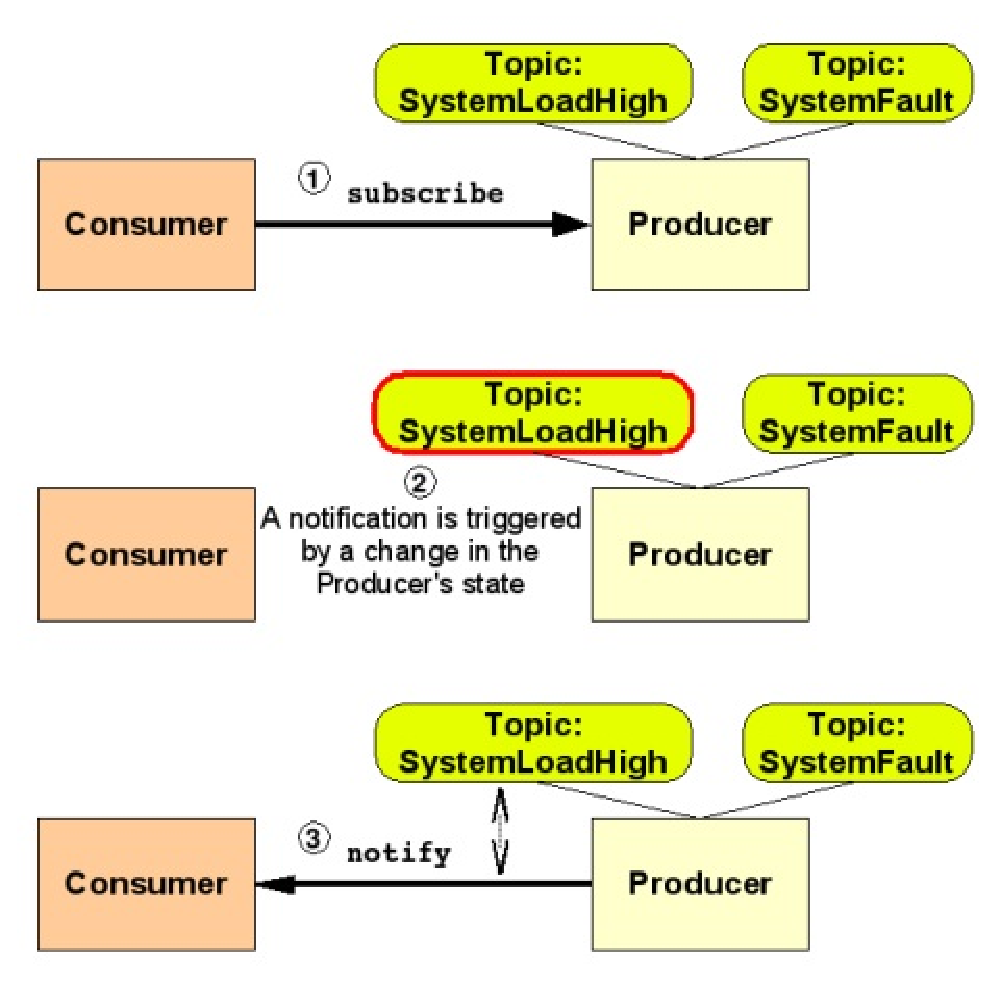
\includegraphics[scale=0.45]{Figures/12}
     \caption{Ejemplo de uso de WS-Notification sin broker.}
  \label{12}
\end{figure}
 
Este caso muestra un ejemplo de interacci�n entre un consumidor y un productor de notificaciones, en el caso de que el suscriptor y el consumidor sean la misma entidad. El sistema es simple ya que tenemos un consumidor y un productor que publica 2 topics: SystemLoadHigh y SystemFault. Los pasos necesarios son: 

\begin{enumerate}
\item En primer lugar, el consumidor se suscribe al topic SystemLoadHigh, por lo que internamente se crea un \emph{Subscription resource} con la informaci�n de la suscripci�n. El productor debe implementar un m�todo \emph{Subscribe} y el consumidor un m�todo \emph{Notify}.  
\item Despu�s, el productor debe enviar una notificaci�n cuando el sistema sobrepase una determinada carga de trabajo. Por ejemplo, nuestro sistema enviar� notificaciones cuando la carga de trabajo sea mayor de 50\%.
\item Por �ltimo, el productor env�a la notificaci�n invocando la operaci�n \emph{Notify} en el consumidor.
\end{enumerate}
   
Un ejemplo de mensaje \emph{Notify} es:
 
\lstset{language=XML, numbersep=5pt, frame=single}
\begin{lstlisting}
...
<wsnt:Notify>
    <wsntw:NotificationMessage>
     <wsnt:Topic Dialect= xsd:anyURI >
       {any}
     </wsnt:Topic>
     <wsnt:ProducerReference>?
      wsa:EndpointReference
     </wsnt:ProducerReference>
     <wsnt:Message>xsd:any</wsnt:Message>
    <wsnt:NotificationMessage>+
</wsnt:Notify>
...
\end{lstlisting}

Como podemos observar el mensaje \emph{Notify} contiene uno o varios mensajes de notificaci�n (\emph{NotificationMessages}). Los campos dentro de �stos son: 

\begin{itemize}
\item Topic: La informaci�n del topic que se env�a.
\item Dialect: El dialecto usado para expresar el topic anterior, es decir, el lenguaje utilizado para expresarlo.
\item ProducerReference: Direcci�n del productor.
\item Message: Una copia de la carga �til (payload) del mensaje actual.
\end{itemize}

A continuaci�n, se muestra el mensaje que manda el suscriptor para registrar su inter�s en uno o m�s topics:


\lstset{language=XML, numbersep=5pt, frame=single}
\begin{lstlisting}
...
<wsnt:Subscribe>
  <wsnt:ConsumerReference>
    wsa:endpointReference
  </wsnt: ConsumerReference>
  <wsnt:TopicExpression Dialect = xsd:anyURI >
    {any}
  </wsnt:TopicExpression>
  <wsnt:UseNotify>xsd:boolean</wsnt:UseNotify>?
  <wsnt:Precondition>wsrp:QueryExpression</Precondition>?
  <wsnt:Selector>wsrp:QueryExpression</wsnt:Selector>?
  <wsnt:SubscriptionPolicy>{any}</wsnt:SubscriptionPolicy>?
  <wsnt:InitialTerminationTime>
    xsd:dateTime
  </wsnt:InitialTerminationTime>?
</wsnt:Subscribe>

...
\end{lstlisting}


Los conceptos importantes en este mensaje son \emph{UseNotify} que se utiliza para decidir si el mensaje de notificaci�n sigue el formalismo WS-Notification o se manda sin formato, \emph{Precondition} que es la condici�n que genera mensajes de notificaci�n, es decir, si se cumple esta condici�n se generan mensajes, pero debe cumplirse tambi�n la condici�n \emph{selector} para enviarlos a los destinatarios que es la que se usa para decidir si se transmiten o no los mensajes generados. Adem�s, \emph{SubscriptionPolicy} se podr�a utilizar para controlar el ratio de env�o de mensajes(por ejemplo, no m�s de 3 por segundo) y \emph{InitialTerminationTime} contiene una sugerencia del tiempo de vida de la suscripci�n. WSRF tambi�n incluye mensajes para detener la suscripci�n, reanudarla o para que un servicio que acaba de unirse a una suscripci�n pueda obtener un historial de notificaciones sobre un determinado topic.



\subsection{WS-BrokeredNotification}

Un \emph{NotificationBroker} es un intermediario que, entre otras cosas, permite el env�o de mensajes entre uno o varios \emph{Publishers} y uno o varios \emph{NotificationConsumers}. La misi�n del \emph{Publisher} es observar ciertas situaciones y crear mensajes de notificaci�n para informar de esas situaciones, mientras que el broker es el encargado de distribuir estos mensajes. \\

En este caso, se pueden dar tres relaciones entre las partes: \emph{simple publishing}, \emph{composable publishing} y \emph{demand-based publishing}. En el primer caso, el \emph{Publisher} es el encargado de observar las situaciones y notificarlas al broker que ser� el encargado de transmitirlas a los interesados. En el segundo caso, el papel del \emph{Publisher} lo realizar� una entidad que implementa una serie de servicios especificados en WS-Notification (NotificationProducer). En este caso, el mensaje de notificaci�n puede llegar a otros consumidores que estuviesen suscritos al productor. En ambos casos, el broker puede pedir al \emph{Publisher} que se registre para poder publicar mensajes sobre un topic determinado. El �ltimo enfoque (\emph{demand-based publishing}) requiere que el \emph{Publisher} sea un \emph{NotificationProducer} y, as�, acepte mensajes de suscripci�n. El objetivo es reducir el n�mero de mensajes de notificaci�n haciendo que �stos solo se manden cuando se soliciten expresamente.


\cleardoublepage

\chapter{Extended Petri nets}\label{chapter:c3}
After introducing web services (and their composition) and the basic formal models
that can be used to model and analyse them, we will focus on this chapter in defining the specific models used in this Thesis. Thus, we
will present the extensions of the basic model of Petri nets stated previously and some properties
that can be analysed. We will recall some notions (marking, firing, enabledness and so on) defined in the preceding chapter
and will adapt them to a particular case. This chapter is mainly divided in two parts. On the one hand,
we will focus on the definition of Coloured Petri nets since they are used in the definition of the language BPELRF, whereas
we will present timed-arc Petri nets, in its two variants (discrete and continuous), as they are the basis of the workflow model presented in the
second part of this Thesis.

\begin{definition} [(General Petri nets)]
A general Petri net is a 5-tuple $N=(P,T,F,K,W)$, where:
\begin{enumerate}
\item $(P,T,F)$ is a basic Petri net.
\item $K\,:\,P \longrightarrow \nnul \,\cup\, \{\infty\}$ is a function that
indicates the maximum number of tokens in each place.
\item $W\,:\,F \longrightarrow \nnul$ is a function that indicates
the multiplicity of the arcs ({\it weight of the arcs}).
\end{enumerate}
When the context is clear, we will call them Petri nets. The function $K$
can be omitted if it is infinite for all the places in the net.
%Adem\'{a}s, es
%usual extender la definici\'{o}n de $W$ a todo el universo de
%posibles arcos, haci\'{e}ndola nula para pares
%$(p,t)$ o $(t,p)$ que no est\'{e}n en $F$.
\end{definition}

\begin{definition} [(Firing rule for general Petri nets)]
Let $N=(P,T,F,K,W)$ be a general Petri net.
\begin{enumerate}
\item A function $M\,:\, P \longrightarrow \nnul$ is a marking
$N$ iff $M(p) \leq K(p)$, for all
$p \in P$.
\item A transition $t \in T$ is enabled in $M$, denoted by $M[ t \rangle$,
iff $W(p,t) \leq M(p) \leq K(p) - W(t,p)$, for all $p \in P$.
The firing of $t$ produces the marking $M'$:
$M'(p) = M(p) - W(p,t) + W(t,p)$, for all $p \in P$.
Again, this evolution is denoted by $M[ t \rangle M'$.
\item A multiset of transitions $R$ is enabled in $M$, written $M [ R \rangle$, if and only if
$M(p) \geq \sum_{t \in T} W(p,t) \cdot R(t)$. The firing of $R$
produces $M'$:
\[ M'(p) = M(p) - \sum_{t \in T} (W(p,t) - W(t,p)) \cdot R(t), \,\,
\forall p \in P\], denoted by $M [ R \rangle M'$.
\end{enumerate}
\end{definition}

\begin{definition} [(Occurrence Sequence)]
Let $N=(P,T,F,K,W,M_0)$ be a marked Petri net.
\begin{enumerate}
\item $\sigma = M_0 t_1 M_1 \ldots t_n M_n$ is a finite occurrence sequence of $N$
if and only if $\forall i \in \{1,\ldots,n\},\,M_{i-1} [ t_i \rangle M_i$.
Occasionally, we will write $t_1 \ldots t_n$, omitting the corresponding markings, since starting from
$M_0$ it is easy to obtain the rest of the markings knowing the transitions fired.
We extend the conventional notation to occurrence sequence, 
obtaining $M_0 [ \sigma \rangle M_n$.
The set of occurrence sequences starting from $M_0$ are denoted by $L(N,M_0)$.

\item An occurrence sequence $\sigma = M_0 R_1 M_1 \ldots R_n M_n$ is finite
iff $\forall i \in \{1,\ldots,n\},\,M_{i-1} [ R_i \rangle M_i$.
%Again, we extend the notation to occurrence sequence, $M_0 [ \sigma \rangle M_n$.
The set of occurrence sequence of $N$ starting from $M_0$ is denoted by $P(N,M_0)$.
\end{enumerate}
\end{definition}

%En lo sucesivo trabajaremos usualmente sobre la sem\'{a}ntica de
%secuencias de ocurrencia, salvo que expl\'{\i}citamente se
%indique lo contrario.

%\bdfn (Matrices de Incidencia)\\
%Sea $N=(P,T,F,W,M_0)$ una Red de Petri Marcada.
%\begin{enumerate}
%\item Se dice que $N$ es {\it pura} sii $\forall t \in T$,
%$\forall p \in P$, $W(t,p) \cdot W(p,t) = 0$.
%\item Si $N$ es una red pura, podemos definir su
%{\it matriz de incidencia previa}, $C^{-} = (c_{i,j}^{-})$,
%$i=1,\ldots,|P|\,;\,j=1,\ldots,|T|$, siendo
%$c_{i,j}^{-} = W(p_i,t_j)$, y su
%{\it matriz de incidencia posterior}
%$C^{+} = (c_{i,j}^{+})$,
%$i=1,\ldots,|P|\,;\,j=1,\ldots,|T|$, siendo
%$c_{i,j}^{+} = W(t_i,p_j)$.
%\item Si $N$ es una red pura se define su {\it matriz de
%incidencia} $C$ por medio de $C = C^+ - C^-$.
%\end{enumerate}
%\edfn

%La matriz de incidencia puede ser definida tambi\'{e}n sobre redes
%que no sean puras, pero en tal caso no caracteriza a las mismas, pues
%una misma matriz de incidencia corresponde a varias redes diferentes.
%
%\bex Es sencillo obtener dos Redes de Petri diferentes con la misma
%matriz de incidencia. Para ello basta tomar
%una Red de Petri Ordinaria y elegir un lugar y una transici\'{o}n
%no conectados inicialmente, y conectarlos formando un loop. Por
%ejemplo, las dos redes de la figura \ref{fig203} tienen la misma
%matriz de incidencia. De hecho, si se trabaja con Redes Generalizadas
%el a\~{n}adido se puede hacer sobre cualquier par.
%\eex
%
%\begin{figure}
%\input{fig28}
%\caption{\label{fig203} Dos Redes de Petri con la misma Matriz de Incidencia}
%\end{figure}

%\bprop (Ecuaci\'{o}n de Estado)\\
%Sea $N=(P,T,F,W,M_0)$ una Red de Petri Marcada Pura,
%$\sigma \in L(N,M_0)$, y $M_0 [ \sigma \rangle M$.
%Entonces se tiene: $M = M_0 + C \cdot \bar{\sigma}$, siendo
%$\bar{\sigma}$ el vector de Parikh asociado a la
%secuencia $\sigma$, que est\'{a} definido como
%$\bar{\sigma}(i) = $n\'{u}mero de ocurrencias de
%la transici\'{o}n $t_i$ en la secuencia $\sigma$.
%
%\proof Sea la secuencia de marcajes producida a lo
%largo de la ejecuci\'{o}n de $\sigma$: $M_0 t_{i_{1}} M_1 \ldots t_{i_{n}} M_n$.
%Entonces, de la regla de disparo se concluye que $M_1 = M_0 +
%C \cdot U_{i_{1}}$, siendo $U_{i_{1}}$ el vector cuyas componentes son todas
%nulas, salvo la $i_{1}$-\'{e}sima, que vale 1. En general, se obtiene
%que $M_k = M_{k-1} + C \cdot U_{i_{k}}$.
%
%Por tanto:
%\[ M_k = M_{k-2} + C \cdot (U_{i_{k-1}} + U_{i_{k}}) = \ldots =
%M_0 + C \cdot \sum_{j=1}^{k} U_{i_{j}}\]
%Ahora bien, $\suma{j=1}{k} U_{i_{j}} = \bar{\sigma}$, lo que
%termina la demostraci\'{o}n.
%\eprop

\section{Petri nets analysis}
When designing a new system, the construction of a graphical model (e.g. a Petri net) of it is always
helpful since it is interesting to broadly understand how this system works. This also helps designers to have a
deeper knowledge about it. Nevertheless, the presence of a graphical model is not enough in many cases
as the designers want the system to meet some properties of interest. For instance, the system is useless
if it reaches a deadlock in each execution.  To this end, it is important to have tools that allow to
evaluate properties in the model. In finite sequential systems, it is not particularly challenging to check
the fulfilment of certain statement, whereas the presence of concurrency complicates this task.
The analysis of systems behaviour is intended to determine the compliance of 
certain properties such as that the number of processes in a queue does not exceed
certain threshold or that the mutual exclusion is guaranteed when accessing to a shared resource.

In Petri nets, one can use a set of powerful tools to formally analyse
the compliance of such properties. Among these tools, designers can check
the absence of deadlocks, the reachability of a certain
state, the possibility of reaching a concrete situation after performing some computations and so on.


\medskip
Normally, these properties are divided in two categories \cite{citar}:

\subsection{Safety properties}
A safety property asserts that \emph{``nothing bad happens''}.
Thus, they guarantee that a set of undesirable states are not reached or that
the system does not execute an unwanted occurrence sequence.

The \emph{safety properties} are the following:

\begin{enumerate}
\item {\bf Reachability}. A marking $M$ of a marked Petri net
$N= (P,T,F,W,M_0)$ is {\it reachable} in $N$
iff there exists an occurrence sequence $\sigma \in L(N,M_0)$
such that $M_0 [ \sigma \rangle M$. We will denote by $[M_0\rangle$ the
set of reachable markings of $N$ starting from $M_0$, and
by $[ M \rangle$ the set of reachable markings starting from the marking $M$.

\item {\bf Boundedness}. A marked Petri net $N=(P,T,F,W,M_0)$ 
is {\it k-bounded}, for some $k \in \nnul$, if all reachable marking
$M$ from $M_0$ hold that $M(p) \leq k$, for all $p \in P$. $N$ is safe if
it is 1-bounded. A place $p \in P$ is
{\it n-safe} if $M(p) \leq n$, for all markings $M$ reachable from $M_0$.

%\item {\bf Boundedness}. Sea
%$N=(P,T,F,W,M_0)$ una Red de Petri Marcada.
%Se dice que un lugar $p \in P$ es limitado si
%existe un n\'{u}mero natural $n \in \nnul$ tal que dicho lugar es
%$n$-seguro; y se dice que $N$ es {\it limitada} si todos sus lugares
%son limitados.
\item {\bf Deadlock-free}. Let $N=(P,T,F,W,M_0)$ a marked Petri net and $M$ be a reachable marking.
$M$ is a {\it dead marking} if there is no $t \in T$ enabled in $M$. 
The net $N$ is deadlock-free iff there are no dead markings.

%\item {\bf Conservaci\'{o}n Respecto a un Vector de Pesos}.
%Sea una Red de Petri Marcada $N=(P,T,F,W,M_0)$, con
%$P = \{p_1,\ldots,p_n\}$. Se dice que $N$ es
%{\it conservativa respecto a un vector de pesos w}, con
%$w \in \nnul^n$, si para todo marcaje alcanzable $M$
%a partir de $M_0$ se cumple:
%\[ \suma{i=1}{n} w_i \cdot M(p_i) =
%\suma{i=1}{n} w_i \cdot M_0(p_i)\]
\item {\bf Coverability}.
Let $N=(P,T,F,W,M_0)$ be a marked Petri net and $M$ be a marking of $N$.
$M$ is said to be {\it coverable} if there exists $M' \in
[M_0 \rangle$ such that $M' \geq M$.
\end{enumerate}

%\noindent {\sc NOTA:} Para ser m\'{a}s precisos, la alcanzabilidad no es
%exactamente una propiedad de seguridad, sino la negaci\'{o}n de la propiedad,
%la no alcanzabilidad. An\'{a}logamente ocurre con el cubrimiento de marcajes.

\subsection{Liveness properties}
A liveness property asserts that \emph{``something good eventually happens''}.
For instance, they guarantee that, independently of the current state of the system,
a specific state can eventually be reached or that a certain occurrence sequence can eventually
be executed in the system.

The \emph{liveness properties} are:
\begin{enumerate}
\item {\bf Liveness}.
Let $N=(P,T,F,W,M_0)$ be a marked Petri net. A transition $t \in T$
is said to be {\it live} if for all reachable marking $M \in
[ M_0 \rangle$ there is an occurrence sequence $\sigma$ starting from $M$ such that
$\sigma = t_1 \ldots t_m$, with $t_m = t$. The $N$ is {\it live} iff all the transitions are live.
\item {\bf Home State}.
Let $N=(P,T,F,W,M_0)$ be a marked Petri net. A marking $M$ of $N$ is a {\it home state} if for all
$M' \in [ M_0 \rangle$, $M \in [ M' \rangle$.
\item {\bf Home Space}. Let $N=(P,T,F,W,M_0)$ be a marked Petri net.
The set of markings ${\cal M}$ is a {\it home-space}
of $N$ if for all marking $M' \in [ M_0 \rangle$ there is marking
$M'' \in {\cal M}$ such that $M'' \in [ M' \rangle$.
\item {\bf Cyclic}.
Let $N=(P,T,F,W,M_0)$ be a marked Petri net. It is said that
$N$ is cyclic if for all marking $M \in [ M_0 \rangle$ there exists an occurrence sequence $\sigma$
starting in $M$ such that $M [ \sigma \rangle M_0$.
\end{enumerate}


% %JIRI % % % %



\section{Timed extensions of Petri nets}

In the
literature on timed extensions of Petri nets we can identify a
first group of models, which assign time delays to transitions,
by using either a fixed deterministic value
\cite{Ram74,Sif77,VFC93} or choosing it from a probability
distribution \cite{AjCh85}. Other models use time intervals to
establish the enabling times of transitions \cite{Mer74}. 
There are also models that introduce time on tokens
\cite{van93,van95,BLT90}. In \cite{Bow96,Wan98} 
a description is given of the different approaches 
to introduce time in Petri nets.

Extender un poco mas esto con información de cada paper


\subsection{Extended Timed-Arc Petri Nets} \label{sec:def}
%We shall now give some preliminaries in order to define the model
%of extended timed-arc Petri nets. 
%We consider only discrete time
%as for closed intervals the reachability/soundness problems
%are equivalent with the continuous time variant as discussed in 
%Section~\ref{sec:cont}.
A \emph{discrete timed transition system} (DTTS) 
is a triple $\left(\proc, \act,\rightarrow\right)$
where $\proc$ is the set of states, $\act$ is the set of actions
and $\rightarrow\: \subseteq \proc \times (\act \cup \nnul)  \times \proc$ is the 
transition relation written as $s \trans{a} s'$ whenever $(s,a,s') \in \rightarrow$. In continuous time,
the transition relation is defined as $\rightarrow\: \subseteq \proc \times (\act \cup \rnul)  \times \proc$.
If $a \in \act$ then we call it a \emph{switch transition}, if
$a \in \nnul$ we call it a \emph{delay transition}.
%By $\rightarrow^{*}$ we denote the reflexive and transitive closure of 
%the relation
%$\rightarrow  \eqdef \bigcup_{a \in \act} \trans{a} \; \cup \; \bigcup_{d \in \nnul} \trans{d}$. 
We also define the set of \emph{well-formed time intervals} 
by: $$\int =\{ [a,a] \;|\; [a,b] \;|\; [a,b) \;|\; (a,b] \;|\; (a,b) \;|\; [a,\infty) \;|\; (a,\infty) \mid a,b \in \nnul,a < b\}$$
Moreover, its subset: $$\intinv = \{ [0,0] \;|\; [0,b] \;|\; [0,b) \;|\; [0,\infty) \mid b \in \nnul\}$$
is used in age invariants. Let us note that we use a discrete time semantics in our definitions 
to avoid the duplication for the case of continuous time. Nevertheless, it is enough to include $\rnul$ instead of $\nnul$ to provide a continuous time semantics.


\begin{definition}[(Extended timed-Arc Petri Net)] \label{defetapn}  
An \emph{extended timed-arc Petri net} 
(ETAPN) is a 9-tuple $N = \tapntuple$ where 
\begin{itemize}
\item $P$ is a finite set of \emph{places},
\item $T$ is a finite set of \emph{transitions} 
such that $P \cap T = \emptyset$, 
\item $\Turg \subseteq T$ is the set of \emph{urgent transitions},
\item $\ia \subseteq P \times T$ is a finite set of \emph{input arcs},
\item $\oa \subseteq T \times P$ is a finite set of \emph{output arcs},
\item $\cfunction : \ia \rightarrow \int$ is a \emph{time constraint function} assigning 
guards %(time intervals) 
to input arcs,
\item $\wfunction : \ia\cup \oa \rightarrow \mathbb{N}$ is a function assigning \emph{weights} to input and output arcs,
\item $\type : \ia \cup \oa \rightarrow \types$ is a \emph{type function} assigning a type to all arcs where $\types = \{\normal, \inhib\} \cup \{\transporti \mid j \in \mathbb{N} \}$ such that  
\begin{itemize}
\item if $\type(a) = \inhib$ then $a \in \ia$ and $\cfunction(a)=[0,\infty]$, 
\item if $(p,t) \in \ia$ and $t \in \Turg$ then $\cfunction((p,t))=[0,\infty]$,
\item if $\type((p,t)) = \transporti$ for some $(p,t) \in \ia$ then there is exactly one $(t,p^{\prime}) \in \oa$ such that $\type((t,p^{\prime})) = 
\transporti$, 
%and moreover $\wfunction((p,t))=\wfunction((t,p^{\prime}))$,
\item if $\type((t,p^{\prime})) = \transporti$ for some $(t,p^{\prime}) \in \oa$ then there is exactly one $(p,t) \in \ia$ such that $\type((p,t)) = 
\transporti$, 
%and moreover $\wfunction((p,t))=\wfunction((t,p^{\prime}))$,
\item if $\type((p,t)) = \transporti = \type((t,p^{\prime}))$ 
then $\wfunction((p,t))=\wfunction((t,p^{\prime}))$,
\end{itemize}
\item $\inv : P \rightarrow \int^{inv}$ is a function assigning \emph{age invariants} to places.
\end{itemize}
\end{definition}

\begin{remark}
Note that for transport arcs we assume that they come in pairs (for
each type $\transporti$) so that their weights match.
Also for inhibitor arcs and for input arcs to urgent transitions, we
require that the guards are $[0,\infty]$. This restriction is important
for some of the results presented in this Thesis and it also guarantees that 
we can use DBM-based algorithms in the tool TAPAAL~\cite{DJJJMS:TACAS:12}.
\end{remark}

The ETAPN model is not monotonic, meaning
that adding more tokens to markings can disable time delays or
transition firing.
Therefore we define a subclass of 
ETAPN where the monotonicity breaking features are not allowed.
In the literature such nets are often considered as the standard
timed-arc Petri net model~\cite{BLT:90,Hanisch:93} but we add the 
prefix monotonic for clarity reasons. 

\begin{definition}[(Monotonic timed-arc Petri net)] \label{deftapn}
A \emph{monotonic timed-arc Petri net} 
(MTAPN) is an extended timed arc Petri net 
with no urgent transitions ($\Turg=\emptyset)$, no age invariants
($\inv(p) = [0,\infty]$ for all $p \in P$) and no 
inhibitor arcs ($\type(a) \not= \inhib$ for all $a \in \ia$).
\end{definition}


%Let $N = \tapntuple$ be a ETAPN and $P^\prime \subseteq P$, the projection $N|_{P^\prime}$ 
%is the net \ensuremath{(P^\prime, T, \ia^\prime,\allowbreak \oa^\prime, \cfunction^\prime, 
%\wfunction^\prime, \type^\prime, \inv^\prime)}, 
%where $\ia^\prime=\ia \cap (P^\prime \times T)$, $\oa^\prime=\oa \cap (T \times P^\prime)$,
%$\cfunction^\prime : \ia^\prime \rightarrow \int$, $\wfunction^\prime : \ia^\prime \cup \oa^\prime \rightarrow \mathbb{N}$,
%$\type^\prime : \ia^\prime \cup \oa^\prime \rightarrow \types$, and $\inv^\prime : P^\prime \rightarrow \int^{inv}$. From now on, we will denote by 
%$P_s$ the set of places shared by various nets. Then, let $N$, $N^\prime$ be two ETAPNs such that $P \cap P^\prime \subseteq P_s$, the disjoint union of $N$ and $N^\prime$ is a ETAPN \ensuremath{(P^{\prime\prime},T^{\prime\prime},\ia^{\prime\prime}, \oa^{\prime\prime},\cfunction^{\prime\prime},\wfunction^{\prime\prime},\type^{\prime\prime}, \inv^{\prime\prime})}, where $P^{\prime\prime}= P\cupdot P^\prime, T^{\prime\prime}=T\cupdot T^\prime, \ia^{\prime\prime}=\ia\cupdot \ia^\prime,\oa^{\prime\prime}=\oa \cupdot \oa^\prime,\cfunction^{\prime\prime}:\ia^{\prime\prime}\cup \oa^{\prime\prime}\rightarrow \int, \wfunction^{\prime\prime}: \ia^{\prime\prime}\cup \oa^{\prime\prime}\rightarrow \mathbb{N}, 
%\type^{\prime\prime} : \ia^{\prime\prime} \cup \oa^{\prime\prime} \rightarrow \types, \text{ and } \inv^{\prime\prime} : P^{\prime\prime} \rightarrow \int^{inv}$.

Before giving the formal semantics of the model, let us fix some notation.
We will recall some definitions presented previously, although applying them
to this kind of nets.
Let $N = \tapntuple$ be an ETAPN. 
%Let $F\eqdef \ia \cup \oa$. 
We denote by ${}^\bullet x \eqdef 
\{y \in P \cup T \mid (y,x) \in (\ia \cup \oa),\ \type((y,x)) \neq \inhib \}$ 
the preset of a transition or a place $x$.
Similarly, the postset $x^\bullet$ is defined as 
$x^\bullet \eqdef \{y \in P \cup T \mid (x,y) \in (\ia \cup \oa) \}$.
Let $\mathcal{B}(\nnul)$ be the set 
of all finite multisets over $\nnul$. A \emph{marking} $M$ on $N$ 
is a function $M : P \longrightarrow \mathcal{B}(\nnul)$ 
where for every place $p \in P$ and 
every token $x \in M(p)$ we have $x \in \inv(p)$. In other words
all tokens have to satisfy the age invariants. 
%The projection of $P^\prime \subseteq P$ in $M$ is a function 
%$M|_{P^\prime} : P^\prime \longrightarrow \mathcal{B}(\nnul)$.
The set of all markings in the net $N$ 
is denoted by $\mathcal{M}(N)$.

We write $(p,x)$ to denote a token at a place $p$ with the 
age $x\in \nnul$. Then $M=\multiset{(p_1,x_1),(p_2,x_2),\dots ,(p_n,x_n)}$ 
is a multiset representing a marking $M$ with $n$ tokens of 
ages $x_i$ in places $p_i$. We 
define the size of a marking as $|M| = \sum_{p\in P}|M(p)|$ where 
$|M(p)|$ is the number of tokens located in the place $p$.

%A marked ETAPN 
%$(N,M_0)$ is a TAPN N together with an initial marking $M_0$ with all tokens of age $0$. 

\begin{definition}[(Enabledness)]
\label{def:enabledness}
 Let $N = \tapntuple$ be an ETAPN. 
We say that a transition $t \in T$ is \emph{enabled} in a marking $M$ by the 
multiset of timed tokens \newline 
$\inn = \multiset{(p,x_{p}^1), (p,x_{p}^2), \dots ,(p,x_{p}^{\wfunction ((p,t))})\mid 
p \in {}^\bullet t} \subseteq M$ and by the multiset of tokens
$\out = \multiset{ (p^{\prime},x_{p^{\prime}}^1),
           (p^{\prime},x_{p^{\prime}}^2),
\dots ,\allowbreak
(p^{\prime},x_{p^{\prime}}^{\wfunction ((t,p^{\prime}))}) 
\mid p^{\prime} \in t^\bullet }$ if
\begin{itemize}
\item for all input arcs except the inhibitor arcs, the tokens from $\inn$ satisfy the age guards of the arcs, i.e. 
%$$\forall(p,t) \in \ia, x_p^i \in \cfunction((p,t))\text{ for }1\leq i\leq w((p,t)) $$ 
$$\forall(p,t) \in \ia. \type((p,t)) \neq \inhib \Rightarrow  x_p^i \in \cfunction((p,t))\text{ for }1\leq i\leq w((p,t)) $$ 
%\item for each place $p$ in ${}^\bullet t$ there are $\wfunction ((p,t))$ tokens from $p$ in $\inn$, i.e. $$\forall p\in {}^\bullet t. \wfunction ((p,t))= n_{p} $$
%\item for each place $p^{\prime}$ in $t^\bullet $ there are $\wfunction ((t,p^{\prime}))$ tokens from $p^{\prime}$ in $\out$, i.e. $$\forall p^{\prime}\in t^\bullet . \wfunction ((t,p^{\prime}))= m_{p^{\prime}} $$
\item for any inhibitor arc pointing from a place $p$ to the
transition $t$, the number of tokens in $p$ is smaller than the weight of the arc, i.e.
$$\forall(p,t) \in \ia. \type((p,t)) = \inhib \Rightarrow|M(p)|<\wfunction ((p,t))$$ 
%$$\forall(p,t) \in \ia. \type((p,t)) = \inhib \Rightarrow \nexists x \in M(p). x \in \cfunction((p,t))$$
\item for all input arcs and output arcs which constitute a transport arc, 
the age of the input token must be equal to the age of the output token and satisfy the invariant of the output place, i.e.
\begin{eqnarray*}
&\forall(p,t) \in \ia. \forall(t,p^{\prime}) \in \oa.\type((p,t)) = \type((t,p^{\prime})) 
= \transporti \\
&\Rightarrow \big( x_p^i = x_{p^{\prime}}^i \wedge x_{p^{\prime}}^i \in 
\inv(p^{\prime})\big) \text{ for } 1\leq i \leq w((p,t))
\end{eqnarray*}
\item for all normal output arcs, the age of the output token is $0$, i.e. $$\forall(t,p^{\prime}) \in \oa. \type((t,p^{\prime})) = \normal \Rightarrow x_{p^{\prime}}^i = 0 \text{ for }1\leq i \leq w((p,t)).$$ 
\end{itemize}
\end{definition}

A given ETAPN $N$ %=\tapntuple$ 
defines a DTTS $T(N)\eqdef (\markingsof(N),T,\rightarrow)$
where states are the markings and the transitions are as follows: 
\begin{itemize}
\item If $t\in T$ is enabled in a marking $M$ by the  multisets of
tokens $\inn$ and $\out$ then $t$ can \emph{fire} and produce 
the marking $M^{\prime} = (M \smallsetminus \inn) \uplus \out$ 
where  $\uplus$ is the multiset sum operator and $\smallsetminus$ is the multiset 
difference operator; we write $M \trans{t} M^{\prime}$ for this 
switch transition.
\item A time \emph{delay} $d \in \nnul$ is allowed in $M$ if
\begin{itemize}
\item $(x+d) \in I(p)$ for all $p \in P$ and for all $x \in M(p)$, and
% i.e. by delaying $d$ time units no token violates any of the age invariants, 
%and
\item if $M \trans{t} M'$ for some $t \in \Turg$ then $d=0$.
 %there is at least one urgent transition enabled in $M$ then
 %     $d=0$, i.e. enabled urgent transitions disallow time passing.
\end{itemize}
By delaying $d$ time units in $M$ we reach the marking $M^{\prime}$ defined as
$M^{\prime}(p) = \multiset{x+d \mid x \in M(p)}$ for all $p \in P$; 
we write $M \trans{d} M^{\prime}$ for this delay transition.
\end{itemize}

%A computation of a net $N$ from the initial marking $M_0$ is
%$M_0 \rightarrow M_1\rightarrow \cdots \rightarrow M_n$ is 
%denoted by $\{M_i\}_{i=0}^{n}$ 
%and we call it a \emph{run}. If the sequence is infinite, we write 
%$\{M_i\}_{i\geq 0}$. Moreover, we write $M \Rightarrow^* M^{\prime}$ if  
%$M^{\prime}$ is reachable from $M$ and $[M\rangle$ represents the set of reachable markings of $M$.

\noindent Let 
$\trans{} \eqdef \bigcup_{t \in T} \trans{t} \cup \bigcup_{d \in \nnul} \trans{d}$.
Again, the set of all markings reachable %in the net $N$ 
from a given marking $M$ is denoted by 
$[M\rangle \eqdef \{ M' \mid M \trans{}^* M' \}$.
By $M \trans{d,t} M'$ we denote that there is a marking $M''$
such that $M \trans{d} M'' \trans{t} M'$.

A marking $M$ is a \emph{deadlock} if there is no $d \in \nnul$ and
no $t \in T$ such that $M \trans{d,t} M'$ 
for some marking $M'$.
A marking $M$ is \emph{divergent} if for any $d \in \nnul$
we have $M \trans{d} M'$ for some $M'$.


%\section{Finite Abstractions for Bounded ETAPNs}

In general, ETAPNs are infinite in two dimensions. The number of tokens
in reachable markings can be unbounded and even for bounded nets
the ages of tokens can be arbitrarily large. 


In PTCPNs, places have an associated colour set (data types). 
Each token has then an attached data value
({\em token colour}),
which belongs to the colour to which the token is
associated. We will use timed colours, for which the first component
will be a non-negative integer value, representing the data value,
and the second component will be the token timestamp,
a natural number representing the time at which the 
token will be available.

There is also a discrete global clock that represents
the total time elapsed in the system model. Moreover, arcs have also 
an associated inscription ({\em arc expressions}),
constructed using variables, constants, operators
and functions. 
To evaluate an arc expression we need to
bind the variables that are part of the expression with their current value, that is, this binding
consists of assigning a value to the variables that appear in the
arc inscription. These values are then used to
select the token colours that must be removed or added when
firing the corresponding transition.

Arc expressions can also have associated time information
both for place-transition and transition-place arcs.
However, only time inscriptions are needed
in output arcs, and even, when all the output arcs
of a transition have the same time inscription,
there is a shorthand notation in CPN Tools
by which this time information is associated with
the transition instead of the output arcs.

The time inscription associated with a transition 
is used to specify the delay that must be added to the
current value of the global clock for
every token generated by the firing of the transition.

Transitions can also have associated guards, which
are Boolean expressions that can prevent their firing.
Thus, when a transition has a guard, it must evaluate to
true for the binding to be enabled,
otherwise the binding is disabled and 
the transition cannot be fired. 

\begin{definition} [(Prioritised-Timed Coloured Petri Nets)]\label{ptcpndef}
A prioritised-timed coloured Petri net is a tuple \ptcpntuple, where: %\footnote{
%We use the classical notation on Petri nets to denote the
%precondition and postcondition of both places and transitions:
%%
%\[ \forall x \in P\,\cup\,T\,:\,
%\precond{x} = \{ y \,|\, (y,x) \in A\}~~~~~
%   x^{\bullet} = \{ y \,|\, (x,y) \in A\}
%\]
%}:
%%
\begin{itemize}
\item $P$ is a finite set of {\em places}, with colours
in the set $\Sigma$. Thus, in our case, colours 
will be pairs $(n,x)\in \nnul \times \nnul$, where $n$ is
the token value and $x$ its timestamp.
%
\item $T$ is a finite set of {\em transitions} ($P\cap T = \emptyset$).
%
\item $A \subseteq (P\times T)\,\cup\,(T \times P)$ is a
set of directed {\em arcs}.
%
\item $\Sigma$ is a finite set of non-empty colour sets. These colour sets can be timed or untimed. For simplicity,
we only use non-negative integer variables and, therefore, the colour sets are: 
$\nnul \times \nnul$ for the timed version and $\nnul$ for the untimed version. Thus, in our case, colours 
will be pairs $(n,x)\in \nnul \times \nnul$ or just $n$, where $n$ is
the token value and $x$ its timestamp.
%
\item $V$ is a finite set of {\em typed variables} in $\Sigma$, 
i.e. ${\it Type}(v) \in \Sigma$, for all $v \in V$.
%
%
\item $G\,:\, T \longrightarrow {\it EXPR}_V$ is the
{\em guard function}, which assigns a Boolean
expression
to each transition, i.e. ${\it Type}(G(t))={\it Bool}$. 
%
\item $E\,:\, A \longrightarrow {\it EXPR}_V$ is the
{\em arc expression function}, which assigns an expression
to each arc, such that ${\it Type}(E(a)) = {\cal B}(\nnul)$,
which corresponds to untimed arcs, since, as mentioned above,
we only attach time delays to transitions.

\item $\lambda$ is the {\em labelling function}, defined
both on places and transitions.

\item $D\,:\,T \longrightarrow \nnul \times \nnul$, which
is the {\em delay function}, which associates a time
interval to each transition. For $D(t)=[d_1,d_2]$,
this means that a uniform probability function will
be used when $t$ is fired to select the specific discrete
delay in that time interval. This is a particularity of CPNTools \cite{CPNTools}.
%
\item $\pi\,:\,T \longrightarrow \nnul$ is the
{\em priority function}, which assigns a priority level
to each transition. In CPNTools, the lower value, the higher priority, that is, $0$ is the highest priority.
\end{itemize}

In this definition, ${\it EXPR}_V$ denotes the
expressions constructed using the variables in $V$,
with the same syntax admitted by CPN Tools. Notice again that we only use here non-negative integer variables for simplicity, but
our model can be easily extended to other variable types.
\end{definition}

\begin{definition} [(Markings)]
Given a PTCPN $N=\ptcpntuple$,
a marking $M$ is defined as a function
$M\,:\,P \longrightarrow {\cal B}(\Sigma)$,
which assigns a multiset of colours to each place
(which can be empty). 

A timed marking of a PTCPN $N$ is a pair $(M,x)$, where
$M$ is a marking of $N$ and $x$ is the current system time instant.
%
%
Initial markings are those markings for which
the timestamp of every token is $0$,
and all variable places are marked with a single
token $(0,0)$.
A marked prioritized-timed coloured Petri net (MPTCPN)
is then defined as a triple $(N,M,x)$, where
$N$ is a PTCPN, and $(M,x)$ a timed marking of it.
%
\end{definition}

We define the semantics for MPTCPNs in a similar way as in \cite{Jensen2009}, 
now taking into account that transitions have associated priorities.
We first introduce the notion of {\em binding}, then
the {\em enabling condition} and finally the {\em firing rule}
for MPTCPNs.

The variables of a transition $t$ are denoted $\mathit{Var(t)\subseteq V}$ and consist of the free variables
appearing in the guard of the transition and in the arc expressions connected to it.

\begin{definition} [(Bindings)]
Let $N=\ptcpntuple$ be a PTCPN.
A {\em binding} of a transition $t \in T$ is a function
$b$ that maps each variable $v \in {\it Var}(t)$
into a value $b(v) \in \Sigma$.
We will denote by $B(t)$ the set of all possible bindings
for the transition $t \in T$. 

Given an expression $e \in {\it EXPR}_V$, we will denote 
by $e\langle b \rangle$ the evaluation of $e$ for the
binding $b$.

A {\em binding element} is then defined as a pair
$(t,b)$, where $t \in T$ and $b \in B(t)$.
The set of all binding elements is denoted by $\mathit{BE}$.
\end{definition}

\begin{definition}[(Enabling condition)]\label{permitidas}
Let $N=\ptcpntuple$ be a PTCPN,
and $(M,x)$ a timed marking of it.
We say that a 
binding element $(t,b) \in \mathit{BE}$
is {\em enabled} at the time instant $x'$ in the timed marking
$(M,x)$ if and
only if the following conditions are fulfilled:

\begin{enumerate}
\item $x' \geq x$.
%
\item $G(t)\langle b \rangle = {\it true}$.
%
\item For all $p \in \precond{t}$,
$E(p,t)\langle b\rangle_{x'} \preceq M(p)$, 
where 
%
$E(p,t)\langle b \rangle_{x'}$ consists of the same
colours as $E(p,t)\langle b \rangle$, but 
replacing their timestamp (which was $0$) by $x'$.
%
%the notation $C_{+x}$ is used to represent the
%colour multiset obtained from $C$ by delaying its timestamps
%by $x$ time units:
%%
%\[
%C_{+x}(n,y) = \left\{
%\begin{array}{cl}
%C(n,y-x)~~ & {\rm if}\;y \geq  x\\
%0        & {\rm otherwise}
%\end{array}
%\right.
%\]
%
\item There is no other binding element $(t',b') \in {\it BE}$
fulfilling the previous conditions  such that $\pi(t') < \pi(t)$.
% INVERTIDAS LAS PRIORIDADES, PARA EVITAR PROBLEMAS,
% AHORA EL CERO ES LA MAXIMA PRIORIDAD.
%
%
\item $x'$ is the smallest time value for which there exists
a binding element $(t,b)$ fulfilling these conditions.
%
\end{enumerate}
%
\end{definition}

\begin{definition} [(Firing rule)]
Let $N=\ptcpntuple$ be a PTCPN,
$(M,x)$ a timed marking of $N$, and an enabled
binding element $(t,b) \in {\it BE}$ at 
instant $x'$ in the timed marking $(M,x)$.

The firing of $(t,b)$ at instant $x'$ is non-deterministic,
depending on the chosen delay $d \in \nnul$ for the transition.
This delay is randomly selected in the interval given by $D(t)$. 
%This delay is chosen according to a uniform probability distribution. 
Thus, the new timed marking $(M',x')$ is: 
%
\[
  \forall p \in P\,:\,
  M'(p) = M(p) \ominus E(p,t)\langle b \rangle_{x'} + E(t,p)\langle b
 \rangle_{d+x'}
\]
%
\end{definition}

\begin{figure}


\hspace*{1.0cm}
\includegraphics[width=11.5cm]{Figures/figure2_scp.eps}
% 
\caption{\label{red1}Graphical view of a PTCPN.}
\end{figure}

\begin{example} Let us consider the marked PTCPN depicted in Figure \ref{red1}, 
obtained from CPNTools examples. 
% 
Observe that timed colour tokens in CPN Tools are drawn
using the notation $n`v@x$,
meaning that we have $n$ instances of a timed colour token 
with colour value $v$ and {\em timestamp} $x$, which correspond to $n.(v,x)$
according to our formal notation. Besides, the symbol `+++'
is there used to represent the union of timed
multisets. 

Thus, $p_{\it in}$ is initially marked with one token
of colour $(3,0)$, and two tokens of colour $(5,0)$,
and the place ${\it rv}$ has one token with colour
$(5,0)$.  Transitions are labelled
with their associated guard, time interval and priority
information. 
Arcs are labelled with the corresponding expressions,
in which no time delays appear, as we are considering
that only transitions have associated time delays.

From the initial marking we can see that
only transition $t_1$ can be fired (at instant $0$), and
any token of those in $p_{\it in}$ can be used for
that purpose.  Taking $(5,0)$ we get the binding $x=5$,
which fulfils the transition guard.
The firing of $t_1$ with this binding removes
one instance of $(5,0)$ from $p_{\it in}$,
and produces a new token on $p_i$.
The timestamp of this new token is a discrete value
in the interval $[1,3]$ (let us say $3$).
Thus, considering the output
arc inscription we get a token $(6,3)$  on $p_i$.

Now, transition $t_1$ must fire again twice (until $p_{\it in}$ 
becomes empty), due to the time constraints of this model. 
As a result we may obtain in $p_i$ the following marking
$\{1.(4,3), 1.(6,1),$
$ 1.(6,3)\}$ (the timestamp values depend on the values
chosen from the interval $[1,3]$).
% 
The only transition that can be fired at this marking
is $t_3$, because due to the time constraints 
we must first use the token $(6,1)$
and $t_2$ cannot be fired using this token.
The firing of $t_3$ produces a new token on $p_{\it ok}$,
whose colour value must be $1$, and the timestamp
depends again on the chosen delay in the time interval
$[1,3]$. For instance, we could obtain the 
colour token $(1,4)$. 

Two tokens now remain in $p_i$, with colours  $(4,3)$ and 
$(6,3)$, and $t_2$ becomes the only transition
enabled (due to condition (4) of Def.\ \ref{permitidas}).
Its firing removes the token $(4,3)$ from $p_i$,
the token on the place ${\it rv}$ changes to $1.(5,3)$,  
and creates a new token on $p_{\it er}$, with colour $(0,3)$. 
%
% 
Finally, the remaining token $(6,3)$ on $p_i$ 
only allows us to fire $t_3$, generating a new token
on $p_{\it ok}$, with value $1$ and a timestamp
depending on the delay chosen for its firing.
\end{example}


%In \cite{Buc03} there is a model that
%extends Merlin's nets by including dynamic priorities and resources.
%
%The particular model that we use is also an extension of Merlin's
%nets, 
%% but it is simpler than that considered in \cite{Buc03}.
%including priorities and three transition types ({\em black,\,grey\,} and
%{\em white\,}). All transitions are assigned both a time interval
%and a static priority. The time interval restricts the instants at
%which a transition is allowed to be fired. {\em White}\, transitions
%are not forced to fire when their clock reaches its latest firing
%time, grey transitions must fire once their clock reaches that value, 
%and black  transitions
%must fire immediately, once they fulfil all the required conditions. 
%Of course, in the
%event of a conflict, any transition of those involved in the conflict 
%can be fired (whichever type it has), although we take into account 
%priorities to resolve the conflicts. Thus, priorities are only
%used in the case of conflict, when at a given marking two or more
%transitions are simultaneously enabled, then only those with 
%the maximum priority are allowed to be fired at that moment.

\cleardoublepage

\chapter{Timed-arc workflow nets}\label{chapter:c4}
\markboth{Chapter~\ref{chapter:c4}.}{}

Recordar incluir los challenges of workflow modelling (resaltar el tiempo y la tool).

\cleardoublepage

\chapter{Timed-arc workflow nets}\label{chapter:c5}
\markboth{Chapter~\ref{chapter:c5}.}{}

In this chapter, we define a framework for modelling business process in terms of timed-arc workflow nets. Here, 
we present a workflow theory based on timed-arc Petri nets,
extend the notion of soundness from~\cite{Aalst97} to deal with 
timing features and introduce a new notion of strong soundness
that guarantees time-bounded workflow termination. We study
the decidability/undecidability of soundness and strong soundness
and conclude that even though they are in general undecidable,
we can still design efficient verification algorithms for two important
subclasses: monotonic workflow nets 
(not using any inhibitor arcs, age invariants and urgent transitions)
and for the subclass of bounded nets. 
This contrasts to the fact that for example the reachability
question for monotonic workflow nets is already 
undecidable~\cite{RGE:reachability}. 
Moreover, our algorithms 
allow us to compute the minimum and maximum execution times of the
workflow. The theory is developed for
discrete-time semantics but in Section~\ref{sec:cont} we discuss its
relationship to the continuous-time semantics. Finally, we implement
the algorithms given here within the open-source tool 
TAPAAL~\cite{DJJJMS:TACAS:12} and successfully demonstrate on a number of 
case studies the applicability of the theory in real-world scenarios.

Analysis of workflow processes with quantitative aspects
like timing is of interest in numerous time-critical applications. 
For instance, workflow nets have been used in various works to provide a formal
model for some WS-BPEL constructions e.g. \cite{AalstJL05,Ouyang2007,AalstL08,LohmannK08,Lohmann07}.
We suggest in this chapter a workflow model based on timed-arc Petri nets and study
the foundational problems of soundness and strong (time-bounded) soundness.
We explore the decidability of these problems
and show, among others, that soundness is decidable for monotonic 
workflow nets while reachability is undecidable.
For general timed-arc workflow nets soundness and
strong soundness become undecidable, though we can design efficient
verification algorithms for the subclass of bounded nets. 
Finally, we compare the discrete and continuous semantics of timed-arc
workflow nets and demonstrate the usability of our theory on
the case studies of a Brake System Control Unit used in aircraft certification,
the MPEG2 encoding algorithm, and 
a blood transfusion workflow.
%, the benchmarking case study of the little-JIL language. 
The implementation of the algorithms is  
freely available as a part of the model checker TAPAAL \cite{tapaal}.

\section{Introduction}
Workflow nets~\cite{Aalst97,Aalst98} were introduced 
by Wil van der Aalst as a formalism
for modelling, analysis and verification of business workflow processes.
%to model, validate and verify business process, \emph{workflow nets} (wf-nets) \cite{Aalst97,Aalst98}. 
The formalism is based on Petri nets abstracting away most of the data 
while focusing on the possible flow in the system. 
Its intended use is in finding design errors 
like the presence of deadlocks, livelocks 
and other anomalies in workflow processes. Such correctness criteria can
be described via the notion of \emph{soundness} (see~\cite{AalstHHSVVW11}) that
requires the option to complete the workflow, guarantees proper termination
and optionally also the absence of redundant tasks. 

After the seminal work on workflow nets, researchers have 
invested much effort in defining new soundness criteria and/or 
improving the expressive power of the original model by adding new features 
and studying the related decidability and 
complexity questions
(it is not in the scope of this paper to list all these works but we
refer to~\cite{AalstHHSVVW11} for a recent overview).
%such as reset or inhibitor arcs, resources, time or multiple instances. 
%It is impossible and is also out of the scope of this paper to summarise here all
%of these works, and, therefore, we refer the interested reader to \cite{AalstHHSVVW11} for further information. 
%Nevertheless, it is worthwhile to
%mention that there is a common characteristic in all of this extended models: undecidability. Thus, soundness (or its different variants)
%is decidable for classical workflow nets \cite{Aalst97}, but, for instance, it is undecidable when we add reset or inhibitor arcs \cite{AalstHHSVVW11}.
In the present paper we consider a quantitative extension of workflow 
nets with timing features, allowing us to argue, among others, 
about the execution intervals of tasks, deadlines and urgent behaviour of workflow processes. Our workflow
model is based on timed-arc Petri nets~\cite{BLT:90,Hanisch:93} 
where tokens carry timing information
and arcs are labelled with time intervals restricting the available
ages of tokens used for transition firing. %We use an extended version
%of the model that allows us to capture advanced timing restrictions
%in a convenient and direct way. 
Let us first informally introduce 
the model on our running example.

The timed-arc workflow net in Figure~\ref{fig:example} 
describes a simple booking-payment workflow
where a web-service provides a booking form followed by online payment.
The whole booking-payment procedure cannot last for more than 10 mi\-nutes
and the booking phase takes at least 2 minutes and 
must be finished within the first 5 minutes. The process can
fail at any moment and the service allows for three additional attempts
before it will terminate with failure. The workflow net 
%in Figure~\ref{fig:example}
consists of six places drawn as circles and nine transitions
drawn as rectangles. Places can contain timed tokens, like the one
of age $0$ in the place $\mathit{in}$ (input place of the workflow).
The tokens present in the net form a marking. 
Places and transitions are connected by arcs
such that arcs from places to transitions contain time intervals restricting
the possible ages of tokens that can be consumed by transition firing.
For simplicity we do not draw time intervals of the form $[0,\infty]$
as they do not restrict the ages of tokens in any way.

\begin{figure}[t]
\begin{tikzpicture}[font=\scriptsize,xscale=1.9,yscale=1.4]
  \tikzstyle{arc}=[->,>=stealth,thick]
	\tikzstyle{transportArc}=[->,>=diamond,thick]
  \tikzstyle{every place}=[minimum size=6mm,thick]
  \tikzstyle{every transition}=[fill=black,minimum width=2mm,minimum height=5mm]
  \tikzstyle{every token}=[fill=white,text=black]
  \tikzstyle{urgency}=[place,fill=white,minimum size=2.0mm,thin]
	\tikzstyle{inhibArc}=[->,>=o,thick]
  \node at (0,0) {};
  \node[place,label=above:$\mathit{in}$] at (0.5,0) (in) {$0$};
	\node[place,label=above:inv: $\leq 5$,] at (1,1.6) (booking) {};
	\node [above] at (1,2.15) {$\mathit{booking}$};
	\node[place,label=above:inv: $\leq 10$] at (3,1.6) (payment) {};
	\node [above] at (3,2.15) {$\mathit{payment}$};
	\node[place,label=above:$\mathit{successful}$] at (5,1.6) (successful) {};
	\node[place,label=above:$\mathit{out}$] at (6,0) (out) {};
	\node[place,label=left:$\mathit{attempts}$] at (2,-1) (attempts) {};
  \node[transition,,rotate=90,] at (1,0) (start) {};
	\node [above] at (0.95,-0.4) {$\mathit{start}$};
  \node[urgency] at (1,0) {};
	\node [above] at (1.55,-0.5) {$3\times$};
  \node[transition,label=$\mathit{book}$] at (2,1.6) (book) {};
  \node[transition,label=$\mathit{pay}$] at (4,1.6) (pay) {}; 
  \node[transition,rotate=90,] at (2,0) (restart1) {}
	 edge [pre, bend right=10, thick,,>=stealth] (booking)
	 edge [pre, thick,>=stealth] (attempts);
 	\draw [->, thick,>=stealth] (restart1) to [bend left=10] (booking);
	\node [above] at (2.35,-0.4) {$\mathit{restart1}$};
	\node[transition,rotate=90,] at (3,0) (restart2) {}
	 edge [pre, thick,>=stealth] (payment)
	 edge [pre, thick,>=stealth] (attempts)
	 edge[post, bend right=10, thick,>=stealth] (booking);
	\node [above] at (3.25,-0.4) {$\mathit{restart2}$};
	\node[transition,rotate=90,] at (4,0) (empty) {}
	 edge [pre, bend left=15, thick,>=stealth] (successful)
	 edge [pre, bend left, thick,>=stealth] (attempts)
	 edge[post, bend right=15, thick,>=stealth] (successful);
	\node[urgency] at (4,0) {};
	\node [above] at (4.25,-0.45) {$\mathit{empty}$};
	\node[transition,rotate=90,] at (5,0) (success) {}
	edge[pre, bend left, >=o, thick](attempts);
  \node[urgency] at (5,0) {};
	\node [above] at (5.25,-0.4) {$\mathit{success}$};
	\node[transition,rotate=90,yshift=0, label=right:$\mathit{fail1\ }$] at (1,-1.5) (fail1) {}
	 edge[pre,>=o, thick](attempts)
	 edge[post, bend right, thick,>=stealth](out);
	\draw[arc] (booking) .. controls (0,1.5) and (0,-1.5) .. (fail1) {};
	\node [above] at (0.05,-0.25) {[5,5]};
	\node[transition,rotate=90,yshift=-0.5, label=right:$\mathit{fail2}$] at (5,-1.5) (fail2) {}
	 edge[pre, bend left=25, thick,>=stealth](payment)
	 edge[pre,>=o, bend left=20, thick](attempts)
	 edge[post, bend right=25, thick,>=stealth](out);
	\node [above] at (3.45,0.52) {[10,10]};
	\draw[arc] (in) -- (start) {};
	\draw[arc] (start) -- (booking) {};
	\draw[transportArc] (booking) -- (book) node[midway,above]{$[2,5]$:1}{};
	\draw[transportArc] (book) -- (payment)  node[midway,above]{:1} {};
	\draw[arc] (payment) -- (pay)  node[midway,above]{$[0,10]$} {};
	\draw[arc] (pay) -- (successful) {};
	\draw[arc] (successful) -- (success) {};
	\draw[arc] (success) -- (out) {};
	\draw[arc] (start) -- (attempts) {};
	%\draw[inhibArc] (attempts) .. controls +(right:3.95cm) and +(-0.2,-1) .. (5,-0.15) {};
		
\end{tikzpicture}
\caption{Booking-payment workflow with timing constraints}
\label{fig:example}
\end{figure}

In the initial marking of the net, the transition $\mathit{start}$
is enabled as it has a token %of an appropriate age 
in its input place.
The transition is urgent (marked with a filled circle), so no time
delay is possible once it gets enabled.
After the $\mathit{start}$ transition is fired, a new token of age 
$0$ arrives to the place $\mathit{booking}$ (initiating the booking phase) 
and three new tokens of age $0$ arrive to the place $\mathit{attempts}$
(in order to count the number of attempts we have before the service fails).
The transition $\mathit{fail1}$ is not enabled as 
the place $\mathit{attempts}$, connected to $\mathit{fail1}$
via the so-called inhibitor arc, contains tokens, inhibiting
$\mathit{fail1}$ from firing. The transition $\mathit{book}$ is not enabled
either as the token's age in the place \itn{booking} 
does not belong to the interval $[2,5]$.
However, after waiting for example $3$ minutes, $\mathit{book}$ %transition 
can fire.  This consumes the token of age $3$ from $\mathit{booking}$ and 
transports it to the place $\mathit{payment}$, preserving its age. This
is signalled by the use of transport arcs that contain the diamond-shaped
tips with index :$1$ (denoting how these arcs are paired). 
%The index is 
%important in a situation when more that one pair of transport arcs is 
%connected to the same transition. If two normal arcs (with standard arrow-shaped tips)
%are used instead of transport arcs, the age of the
%token would be reset to $0$ after being it transported to the place
%$\mathit{payment}$. As we, however, used transport arcs,
%we know that the transition $\mathit{pay}$ can be fired within 
%at most $10$ minutes since the whole booking-payment service started.

At any moment, the booking-payment part of the workflow can be
restarted by firing the transitions $\mathit{restart1}$ or
$\mathit{restart2}$. This will bring the token back to the place
$\mathit{booking}$, reset its age to $0$, and consume one attempt from
the place $\mathit{attempts}$. Once no more attempts are available
and the age of the token in the place $\mathit{booking}$ or
$\mathit{payment}$ reaches $5$ resp. $10$, we can fire
the transition $\mathit{fail1}$ resp. $\mathit{fail2}$ and terminate the
workflow by placing a token into the output place $\mathit{out}$.
Note that the places $\mathit{booking}$ and $\mathit{payment}$ contain
age invariants $\leq 5$ resp. $\leq 10$, meaning that the ages of tokens in 
these places should be at most $5$ resp. $10$. Hence if the service
did not succeed within the given time bound, the workflow will necessarily
fail.
Finally, if the payment transition was executed within 10 minutes
from the service initialization, the transition
$\mathit{empty}$ can now repeatedly remove any remaining tokens in the place
$\mathit{attempts}$ and the transition $\mathit{success}$ terminates 
the whole workflow. As both the transitions
$\mathit{empty}$ and $\mathit{success}$ are urgent, no further time delay
is allowed in this termination phase.
%after the execution of the transition $\mathit{pay}$.

We are concerned with the study of
soundness and strong soundness, intuitively meaning that from any
marking reachable from the initial one, it is always possible
to reach a marking (in case of strong soundness additionally within a fixed
amount of time), having just one token in the place $\itn{out}$.
Moreover, once a token appears in the place $\itn{out}$, it is mandatory
that the rest of the workflow net does not contain any remaining tokens.
One can verify (either manually or using our tool mentioned later)
that the workflow net of our running example is both sound and strongly sound.

\paragraph{Our contribution.}
We define a workflow theory based on timed-arc Petri nets,
extend the notion of soundness from~\cite{Aalst97} to deal with 
timing features and introduce a new notion of strong soundness
that guarantees time-bounded workflow termination. We study
the decidability/undecidability of soundness and strong soundness
and conclude that even though they are in general undecidable,
we can still design efficient verification algorithms for two important
subclasses: monotonic workflow nets 
(not using any inhibitor arcs, age invariants and urgent transitions)
and for the subclass of bounded nets. 
This contrasts to the fact that for example the reachability
question for monotonic workflow nets is already 
undecidable~\cite{RGE:reachability}. 
Moreover, our algorithms 
allow us to compute the minimum and maximum execution times of the
workflow. The theory is developed for
discrete-time semantics but in Section~\ref{sec:cont} we discuss its
relationship to the continuous-time semantics. Finally, we implement
the algorithms given in this paper within the open-source tool 
TAPAAL~\cite{DJJJMS:TACAS:12} and successfully demonstrate on a number of 
case studies the applicability of the theory in real-world scenarios.

\section*{Related Work}

Soundness for different extensions of Petri nets with e.g. 
inhibitor arcs, reset arcs and other features have been studied before,
leading often to undecidability results (for a detailed overview 
see~\cite{AalstHHSVVW11}). We shall now focus mainly on 
time extensions of Petri net workflow models.
%nets as modelling tool. On the one hand, there are a bunch of works 
%defining timed workflows nets in terms of time Petri nets, that is, 
%an interval is associated to the firing of a transition.
Ling and Schmidt~\cite{LS2000} defined timed workflow nets in terms 
of Time Elementary Nets (TENs). These nets are 1-bounded by definition 
and a net is sound iff it is live and the initial marking is a
home marking in a net that connects the output place of the workflow with
the input one. Du and Jiang~\cite{DuJ03} suggested Logical Time Workflow Nets 
(LTWN) and their compositional semantics. Here liveness together with 
boundedness is a necessary and sufficient condition for soundness.
Moreover, the soundness of a well-structured LTWN can be verified 
in polynomial time. Tiplea et al.~\cite{TipleaM05} 
introduced a variant of timed workflow nets in terms of timed Petri nets 
and showed the decidability of soundness for the bounded subclass.
In subsequent work~\cite{TipleaM06,TipleaM09} they studied the decidability 
of soundness under different firing strategies. The papers listed above
rely on the model of time Petri nets where timing information is
associated to transitions and not to tokens like in our case.
The two models are significantly different, in particular the 
number of timing parameters for time Petri nets is fixed, contrary
to the dynamic creation of tokens with their private clocks in
timed-arc Petri nets. We also see several modelling advantages
of having ages associated to tokens as we can for example track
the duration of sequentially composed tasks (via transport arcs) 
as demonstrated in our running example. We are not aware of other
works developing a workflow theory and the corresponding notions
of soundness based on timed-arc Petri nets. Finally, we
implement the soundness checks within a user-friendly tool
that permits easy GUI-based debugging of issues in workflows---something 
that is not that common for other workflow analysis tools 
(see~\cite{FF:AWPN:06} for more discussion).

\section{Timed-Arc Workflow Petri Nets} \label{sec:def}
%We shall now give some preliminaries in order to define the model
%of extended timed-arc Petri nets. 
%We consider only discrete time
%as for closed intervals the reachability/soundness problems
%are equivalent with the continuous time variant as discussed in 
%Section~\ref{sec:cont}.
%Let $\nnul = \mathbb{N} \cup \{0\}$ and 
%$\nnul^{\infty} = \nnul \cup \left\{\infty \right\}$.
%A \emph{discrete timed transition system} (DTTS) 
%is a triple $\left(\proc, \act,\rightarrow\right)$
%where $\proc$ is the set of states, $\act$ is the set of actions
%and $\rightarrow\: \subseteq \proc \times (\act \cup \nnul)  \times \proc$ is the 
%transition relation written as $s \trans{a} s'$ whenever $(s,a,s') \in \rightarrow$.
%If $a \in \act$ then we call it a \emph{switch transition}, if
%$a \in \nnul$ we call it a \emph{delay transition}.
%%By $\rightarrow^{*}$ we denote the reflexive and transitive closure of 
%%the relation
%%$\rightarrow  \eqdef \bigcup_{a \in \act} \trans{a} \; \cup \; \bigcup_{d \in \nnul} \trans{d}$. 
%We also define the set of \emph{well-formed time intervals} as 
%$\int \eqdef \{[a,b] \mid a \in \nnul,b\in \nnul^{\infty}, a\leq b \}$
%and its subset $\intinv \eqdef \{[0,b] \mid b\in \nnul^{\infty} \}$
%used in age invariants. 

%%% Nice intro but repeats too much from introduction, do not remove it though
%We can now introduce the timed-arc Petri net model
%where each token carries its own
%age and input arcs to transitions are annotated with time intervals
%that restrict the ages of tokens usable for transition firing. Newly
%produced tokens become of age $0$, unless they were produced by
%a pair of so-called \emph{transport arcs} that describe
%a path along which the tokens travel from input to output places 
%while preserving the ages of the tokens moved along the path. In this paper
%we study an extended model with (i) \emph{age invariants}
%associated to places that restrict the maximal possible ages of tokens
%in the given places, (ii) \emph{inhibitor arcs} that as in normal Petri
%nets inhibit transition firing, and
%(iii) \emph{urgent transitions} that disable time delay whenever
%at least one of them is enabled.
%These additional extensions add a considerable expressive power
%(as also demonstrated by the decidability and undecidability results
%proved in this paper) and they are essential for convenient modelling 
%of systems with timing attributes.

%\begin{definition}[Extended timed-Arc Petri Net] \label{defetapn}  
%An \emph{extended timed-arc Petri net} 
%(ETAPN) is a 9-tuple $N = \tapntuple$ where 
%\begin{itemize}
%\item $P$ is a finite set of \emph{places},
%\item $T$ is a finite set of \emph{transitions} 
%such that $P \cap T = \emptyset$, 
%\item $\Turg \subseteq T$ is the set of \emph{urgent transitions},
%\item $\ia \subseteq P \times T$ is a finite set of \emph{input arcs},
%\item $\oa \subseteq T \times P$ is a finite set of \emph{output arcs},
%\item $\cfunction : \ia \rightarrow \int$ is a \emph{time constraint function} assigning 
%guards %(time intervals) 
%to input arcs,
%\item $\wfunction : \ia\cup \oa \rightarrow \mathbb{N}$ is a function assigning \emph{weights} to input and output arcs,
%\item $\type : \ia \cup \oa \rightarrow \types$ is a \emph{type function} assigning a type to all arcs where $\types = \{\normal, \inhib\} \cup \{\transporti \mid j \in \mathbb{N} \}$ such that  
%\begin{itemize}
%\item if $\type(a) = \inhib$ then $a \in \ia$ and $\cfunction(a)=[0,\infty]$, 
%\item if $(p,t) \in \ia$ and $t \in \Turg$ then $\cfunction((p,t))=[0,\infty]$,
%\item if $\type((p,t)) = \transporti$ for some $(p,t) \in \ia$ then there is exactly one $(t,p^{\prime}) \in \oa$ such that $\type((t,p^{\prime})) = 
%\transporti$, 
%%and moreover $\wfunction((p,t))=\wfunction((t,p^{\prime}))$,
%\item if $\type((t,p^{\prime})) = \transporti$ for some $(t,p^{\prime}) \in \oa$ then there is exactly one $(p,t) \in \ia$ such that $\type((p,t)) = 
%\transporti$, 
%%and moreover $\wfunction((p,t))=\wfunction((t,p^{\prime}))$,
%\item if $\type((p,t)) = \transporti = \type((t,p^{\prime}))$ 
%then $\wfunction((p,t))=\wfunction((t,p^{\prime}))$,
%\end{itemize}
%\item $\inv : P \rightarrow \int^{inv}$ is a function assigning \emph{age invariants} to places.
%\end{itemize}
%\end{definition}
%
%\begin{remark}
%Note that for transport arcs we assume that they come in pairs (for
%each type $\transporti$) so that their weights match.
%Also for inhibitor arcs and for input arcs to urgent transitions, we
%require that the guards are $[0,\infty]$. This restriction is important
%for some of the results presented in this paper and it also guarantees that 
%we can use DBM-based algorithms in the tool TAPAAL~\cite{DJJJMS:TACAS:12}.
%\end{remark}
%
%The ETAPN model is not monotonic, meaning
%that adding more tokens to markings can disable time delays or
%transition firing.
%Therefore we define a subclass of 
%ETAPN where the monotonicity breaking features are not allowed.
%In the literature such nets are often considered as the standard
%timed-arc Petri net model~\cite{BLT:90,Hanisch:93} but we add the 
%prefix monotonic for clarity reasons. 
%
%\begin{definition}[Monotonic timed-arc Petri net] \label{deftapn}
%A \emph{monotonic timed-arc Petri net} 
%(MTAPN) is an extended timed arc Petri net 
%with no urgent transitions ($\Turg=\emptyset)$, no age invariants
%($\inv(p) = [0,\infty]$ for all $p \in P$) and no 
%inhibitor arcs ($\type(a) \not= \inhib$ for all $a \in \ia$).
%\end{definition}


%Let $N = \tapntuple$ be a ETAPN and $P^\prime \subseteq P$, the projection $N|_{P^\prime}$ 
%is the net \ensuremath{(P^\prime, T, \ia^\prime,\allowbreak \oa^\prime, \cfunction^\prime, 
%\wfunction^\prime, \type^\prime, \inv^\prime)}, 
%where $\ia^\prime=\ia \cap (P^\prime \times T)$, $\oa^\prime=\oa \cap (T \times P^\prime)$,
%$\cfunction^\prime : \ia^\prime \rightarrow \int$, $\wfunction^\prime : \ia^\prime \cup \oa^\prime \rightarrow \mathbb{N}$,
%$\type^\prime : \ia^\prime \cup \oa^\prime \rightarrow \types$, and $\inv^\prime : P^\prime \rightarrow \int^{inv}$. From now on, we will denote by 
%$P_s$ the set of places shared by various nets. Then, let $N$, $N^\prime$ be two ETAPNs such that $P \cap P^\prime \subseteq P_s$, the disjoint union of $N$ and $N^\prime$ is a ETAPN \ensuremath{(P^{\prime\prime},T^{\prime\prime},\ia^{\prime\prime}, \oa^{\prime\prime},\cfunction^{\prime\prime},\wfunction^{\prime\prime},\type^{\prime\prime}, \inv^{\prime\prime})}, where $P^{\prime\prime}= P\cupdot P^\prime, T^{\prime\prime}=T\cupdot T^\prime, \ia^{\prime\prime}=\ia\cupdot \ia^\prime,\oa^{\prime\prime}=\oa \cupdot \oa^\prime,\cfunction^{\prime\prime}:\ia^{\prime\prime}\cup \oa^{\prime\prime}\rightarrow \int, \wfunction^{\prime\prime}: \ia^{\prime\prime}\cup \oa^{\prime\prime}\rightarrow \mathbb{N}, 
%\type^{\prime\prime} : \ia^{\prime\prime} \cup \oa^{\prime\prime} \rightarrow \types, \text{ and } \inv^{\prime\prime} : P^{\prime\prime} \rightarrow \int^{inv}$.

%Before we give the formal semantics of the model, let us fix some notation.
%Let $N = \tapntuple$ be an ETAPN. 
%%Let $F\eqdef \ia \cup \oa$. 
%We denote by ${}^\bullet x \eqdef 
%\{y \in P \cup T \mid (y,x) \in (\ia \cup \oa),\ \type((y,x)) \neq \inhib \}$ 
%the preset of a transition or a place $x$.
%Similarly, the postset $x^\bullet$ is defined as 
%$x^\bullet \eqdef \{y \in P \cup T \mid (x,y) \in (\ia \cup \oa) \}$.
%Let $\mathcal{B}(\nnul)$ be the set 
%of all finite multisets over $\nnul$. A \emph{marking} $M$ on $N$ 
%is a function $M : P \longrightarrow \mathcal{B}(\nnul)$ 
%where for every place $p \in P$ and 
%every token $x \in M(p)$ we have $x \in \inv(p)$, in other words
%all tokens have to satisfy the age invariants. 
%%The projection of $P^\prime \subseteq P$ in $M$ is a function 
%%$M|_{P^\prime} : P^\prime \longrightarrow \mathcal{B}(\nnul)$.
%The set of all markings in a net $N$ 
%is denoted by $\mathcal{M}(N)$.
%
%We write $(p,x)$ to denote a token at a place $p$ with the 
%age $x\in \nnul$. Then $M=\{(p_1,x_1),(p_2,x_2),\dots ,(p_n,x_n)\}$ 
%is a multiset representing a marking $M$ with $n$ tokens of 
%ages $x_i$ in places $p_i$. We 
%define the size of a marking as $|M| = \sum_{p\in P}|M(p)|$ where 
%$|M(p)|$ is the number of tokens located in the place $p$.
%
%%A marked ETAPN 
%%$(N,M_0)$ is a TAPN N together with an initial marking $M_0$ with all tokens of age $0$. 
%
%\begin{definition}[Enabledness]
%\label{def:enabledness}
% Let $N = \tapntuple$ be an ETAPN. 
%We say that a transition $t \in T$ is \emph{enabled} in a marking $M$ by the 
%multisets of tokens
%$\inn = \{(p,x_{p}^1), (p,x_{p}^2), \dots ,(p,x_{p}^{\wfunction ((p,t))})\mid 
%p \in {}^\bullet t\} \subseteq M$ and 
%$\out = \{ (p^{\prime},x_{p^{\prime}}^1),
%           (p^{\prime},x_{p^{\prime}}^2),
%\dots ,\allowbreak
%(p^{\prime},x_{p^{\prime}}^{\wfunction ((t,p^{\prime}))}) 
%\mid p^{\prime} \in t^\bullet \}$ if
%\begin{itemize}
%\item for all input arcs except the inhibitor arcs, the tokens from $\inn$ satisfy the age guards of the arcs, i.e. 
%%$$\forall(p,t) \in \ia, x_p^i \in \cfunction((p,t))\text{ for }1\leq i\leq w((p,t)) $$ 
%$$\forall(p,t) \in \ia. \type((p,t)) \neq \inhib \Rightarrow  x_p^i \in \cfunction((p,t))\text{ for }1\leq i\leq w((p,t)) $$ 
%%\item for each place $p$ in ${}^\bullet t$ there are $\wfunction ((p,t))$ tokens from $p$ in $\inn$, i.e. $$\forall p\in {}^\bullet t. \wfunction ((p,t))= n_{p} $$
%%\item for each place $p^{\prime}$ in $t^\bullet $ there are $\wfunction ((t,p^{\prime}))$ tokens from $p^{\prime}$ in $\out$, i.e. $$\forall p^{\prime}\in t^\bullet . \wfunction ((t,p^{\prime}))= m_{p^{\prime}} $$
%\item for any inhibitor arc pointing from a place $p$ to the
%transition $t$, the number of tokens in $p$ is smaller than the weight of the arc, i.e.
%$$\forall(p,t) \in \ia. \type((p,t)) = \inhib \Rightarrow|M(p)|<\wfunction ((p,t))$$ 
%%$$\forall(p,t) \in \ia. \type((p,t)) = \inhib \Rightarrow \nexists x \in M(p). x \in \cfunction((p,t))$$
%\item for all input arcs and output arcs which constitute a transport arc, 
%the age of the input token must be equal to the age of the output token and satisfy the invariant of the output place, i.e.
%\begin{eqnarray*}
%&\forall(p,t) \in \ia. \forall(t,p^{\prime}) \in \oa.\type((p,t)) = \type((t,p^{\prime})) 
%= \transporti \\
%&\Rightarrow \big( x_p^i = x_{p^{\prime}}^i \wedge x_{p^{\prime}}^i \in 
%\inv(p^{\prime})\big) \text{ for } 1\leq i \leq w((p,t))
%\end{eqnarray*}
%\item for all normal output arcs, the age of the output token is $0$, i.e. $$\forall(t,p^{\prime}) \in \oa. \type((t,p^{\prime})) = \normal \Rightarrow x_{p^{\prime}}^i = 0 \text{ for }1\leq i \leq w((p,t)).$$ 
%\end{itemize}
%\end{definition}
%
%A given ETAPN $N$ %=\tapntuple$ 
%defines a DTTS $T(N)\eqdef (\markingsof(N),T,\rightarrow)$
%where states are the markings and the transitions are as follows. 
%\begin{itemize}
%\item If $t\in T$ is enabled in a marking $M$ by the  multisets of
%tokens $\inn$ and $\out$ then $t$ can \emph{fire} and produce 
%the marking $M^{\prime} = (M \smallsetminus \inn) \uplus \out$ 
%where  $\uplus$ is the multiset sum operator and $\smallsetminus$ is the multiset 
%difference operator; we write $M \trans{t} M^{\prime}$ for this 
%switch transition.
%\item A time \emph{delay} $d \in \nnul$ is allowed in $M$ if
%\begin{itemize}
%\item $(x+d) \in I(p)$ for all $p \in P$ and all $x \in M(p)$, and
%% i.e. by delaying $d$ time units no token violates any of the age invariants, 
%%and
%\item if $M \trans{t} M'$ for some $t \in \Turg$ then $d=0$.
% %there is at least one urgent transition enabled in $M$ then
% %     $d=0$, i.e. enabled urgent transitions disallow time passing.
%\end{itemize}
%By delaying $d$ time units in $M$ we reach the marking $M^{\prime}$ defined as
%$M^{\prime}(p) = \{x+d \mid x \in M(p)\}$ for all $p \in P$; 
%we write $M \trans{d} M^{\prime}$ for this delay transition.
%\end{itemize}
%
%%A computation of a net $N$ from the initial marking $M_0$ is
%%$M_0 \rightarrow M_1\rightarrow \cdots \rightarrow M_n$ is 
%%denoted by $\{M_i\}_{i=0}^{n}$ 
%%and we call it a \emph{run}. If the sequence is infinite, we write 
%%$\{M_i\}_{i\geq 0}$. Moreover, we write $M \Rightarrow^* M^{\prime}$ if  
%%$M^{\prime}$ is reachable from $M$ and $[M\rangle$ represents the set of reachable markings of $M$.
%
%\noindent Let 
%$\trans{} \eqdef \bigcup_{t \in T} \trans{t} \cup \bigcup_{d \in \nnul} \trans{d}$.
%The set of all markings reachable %in the net $N$ 
%from a given marking $M$ is denoted by 
%$[M\rangle \eqdef \{ M' \mid M \trans{}^* M' \}$.
%By $M \trans{d,t} M'$ we denote that there is a marking $M''$
%such that $M \trans{d} M'' \trans{t} M'$.
%
%A marking $M$ is a \emph{deadlock} if there is no $d \in \nnul$ and
%no $t \in T$ such that $M \trans{d,t} M'$ 
%for some marking $M'$.
%A marking $M$ is \emph{divergent} if for any $d \in \nnul$
%we have $M \trans{d} M'$ for some $M'$.


%\section{Finite Abstractions for Bounded ETAPNs}

In this section, we provide the formal definition of timed-arc workflow nets. This model is based on the 
timed-arc Petri nets defined in Chapter \ref{chapter:c3}. After that, we recall the soundness definition, extending it
to the time setting. Moreover, we present some important definitions (cut markings, maximum constant,etc) 
to completely understand the theory presented here.

In general, ETAPNs are infinite in two dimensions. The number of tokens
in reachable markings can be unbounded and even for bounded nets
the ages of tokens can be arbitrarily large. We shall now recall a 
few results that allow us to make finite abstractions for bounded
ETAPNs, i.e. for nets where the maximum number of tokens in any
reachable marking is bounded by a constant.

Let $N=\tapntuple$ be a given ETAPN.
In~\cite{ALSST:MEMICS:12} 
the authors provide an algorithm for computing 
a function $\cmax: P \rightarrow (\nnul \cup \{ -1 \})$ 
returning for each place $p \in P$ the maximum constant associated
to this place, meaning that the ages of tokens in place $p$ that
are strictly greater than $\cmax(p)$ are irrelevant. In particular,
places where $\cmax(p)=-1$ are the so-called \emph{untimed} places
where the age of tokens is not relevant at all, implying that all
the intervals on their ongoing arcs are $[0,\infty]$.

Let $M$ be a marking of $N$. We split it into 
two markings $\mold$ and $\myoung$ where 
$\mold (p)=\left\{ x\in M(p) \mid x>\cmax(p) \right\}$ 
and $\myoung (p)=\allowbreak\left\{ x\in M(p) \mid 
x\allowbreak\leq\allowbreak \cmax(p) \right\}$
for all places $p \in P$. Clearly,
$M = \mold \uplus \myoung$.

We say that two markings $M$ and $M'$ in the net $N$ are equivalent, 
written $M \eqMarking M^{\prime}$, 
if $\myoung=\myoung^{\prime}$
and for all $p \in P$ we have
$|\mold (p)|=|\mold^{\prime}(p)|$.
In other words $M$ and $M'$ agree on the tokens with ages below the
maximum constants and have the same number of tokens above the maximum
constant.
% (relevant only for places $p$ with $I(p)=[0,\infty]$ as
%places with nontrivial age invariants cannot have tokens older that 
%the maximum constant which is in this case equal to the invariant upper-bound).

The relation $\eqMarking$ is an equivalence relation and it is
also a timed bisimulation 
where delays and transition firings on one side can be matched by
exactly the same delays and transition firings on the other side
and vice versa. % (see e.g.~\cite{LY:97}).

\begin{theorem}[\cite{ALSST:MEMICS:12}]
\label{thm:bisim}
  The relation $\eqMarking$ is a timed bisimulation.
\end{theorem}

We can now define canonical representatives for each
equivalence class of $\eqMarking$. 

\begin{definition}[Cut]
\label{def:cut}
Let $M$ be a marking.
We define its canonical marking $\cut(M)$ by 
$\cut(M)(p)= \myoung(p)\uplus \big\{ \underbrace{ \cmax(p)+1,\dots ,\cmax(p)+1 }_{|\mold(p)| \text{ times}} \big\}$.
%\begin{equation*}
%  \cut(M)(p)=
%\begin{cases}
%\myoung(p)  \quad \text{if $p$ is invariant or dead-token place,} \\
%\myoung(p)\uplus \big\{ \underbrace{ \cmax(p)+1,\dots ,\cmax(p)+1 }_{|\mold(p)| \text{ times}} \big\}    \quad \text{if $p$ is a normal place.}
%\vspace{-.45cm}
%\end{cases}
%\vspace{.45cm}
%\end{equation*}
\end{definition}

\begin{lemma}[\cite{ALSST:MEMICS:12}]
\label{lemma:canon}
Let $M$, $M_1$ and $M_2$ be markings. Then
(i) $M \eqMarking \cut(M)$, and (ii)
$M_1 \eqMarking M_2$ if and only if $\cut(M_1)=\cut(M_2)$.
\end{lemma}

Let $M$ and $M^\prime$ be two markings. We say that $M^\prime$ \emph{covers} 
$M$, denoted by $M \sqsubseteq M^\prime$, if $M(p) \subseteq M^\prime(p)$ 
for all $p \in P$. We write $M \sqsubseteq_{cut} M^\prime$ 
if $cut(M) \sqsubseteq cut(M^\prime)$.

For monotonic timed-arc Petri nets we can now show that adding more tokens
to the net does not restrict its possible behaviour. 

\begin{lemma}
\label{lem:mono}
Let $N$ be an MTAPN and $M,M' \in \mathcal{M}(N)$
be two of its markings such that $M \sqsubseteq_{\cut} M'$. 
If $M \trans{d} M_1$ (resp. $M \trans{t} M_1$) then 
$M' \trans{d} M'_1$ (resp. $M' \trans{t} M'_1$) such that 
$M_1 \sqsubseteq_{cut} M'_1$ and 
$|M'|-|M|=|M'_1|-|M_1|$.
\end{lemma}
\begin{proof}
Let $M \trans{d} M_1$, resp. $M \trans{t} M_1$.
As $M \equiv \cut(M)$ by Lemma~\ref{lemma:canon}(i),
we can by Theorem~\ref{thm:bisim} conclude that also $\cut(M) \trans{d} M_2$,
resp. $\cut(M) \trans{t} M_2$,
such that $M_1 \equiv M_2$. Recall that $\cut(M) \sqsubseteq \cut(M')$
by the assumption of the lemma.
\begin{itemize}
\item Time delay case ($\cut(M) \trans{d} M_2$).
As the net does not contain any nontrivial age invariants
and there are no urgent transitions,
we know that also $\cut(M') \trans{d} M_3$ such that
$M_2 \sqsubseteq M_3$ as time delay preserves the $\sqsubseteq$-relation.
\item Transition firing case ($\cut(M) \trans{t} M_2$).
As the net does not have any inhibitor arcs,
we can see that also $\cut(M') \trans{t} M_3$ by consuming
exactly the same tokens in $\cut(M')$ as we did in $\cut(M)$.
Clearly, $M_2 \sqsubseteq M_3$.
\end{itemize}
Because $\cut(M') \equiv M'$ due to Lemma~\ref{lemma:canon}(i),
we know by Theorem~\ref{thm:bisim}
that $M' \trans{d} M'_1$, resp. $M' \trans{t} M'_1$, such that $M_3 \equiv M'_1$.
Hence $M_1 \equiv M_2 \sqsubseteq M_3 \equiv M'_1$.
By Lemma~\ref{lemma:canon}(ii) we get
$\cut(M_1)=\cut(M_2)$ and $\cut(M_3)=\cut(M'_1)$.
Observe now a simple fact that $M_2 \sqsubseteq M_3$ implies that
$\cut(M_2) \sqsubseteq \cut(M_3)$.
This all together implies that $\cut(M_1)=\cut(M_2) \sqsubseteq
\cut(M_3) = \cut(M'_1)$ which is another way of saying that
$M_1 \sqsubseteq_\cut M'_1$ as required by the lemma.
As time delays do not change the number of
tokens in $M$ and $M'$ and transition firing adds or removes an
equal number of tokens from both $M$ and $M'$,
we can also conclude that $|M'|-|M|=|M'_1|-|M_1|$.
\qed
\end{proof}




%%%%%%%%%%%%%%%%%%%%%% Section%%%%%%%%%%%%%%%%%%%%%%%%%%%%%
Timed-arc workflow nets are defined similarly as untimed 
workflow nets~\cite{Aalst97}. Every workflow net has a unique
input place and a unique output place. After initializing such a 
net by placing a token into the input place, it should be
guaranteed that any possible workflow execution can be always 
extended such that the workflow terminates with just one token
in the output place (also known as the soundness property).

% with the notion of time associated to the tokens in the net.

\begin{definition}[Extended timed-arc workflow net] \label{defetawfn}
An \itn{ETAPN} $N=\tapntuple$ is called an 
\emph{Extended Timed-Arc WorkFlow Net} (ETAWFN) 
if
\begin{itemize}
\item there exists a unique place $in \in P$ such that $^\bullet in= \emptyset$ and $in^\bullet \neq \emptyset$,
\item there exists a unique place $out \in P$ such that $out^\bullet=\emptyset$ and $^\bullet out \neq \emptyset$,
%\item $\forall t \in T$, there is a path from {\it in} to {\it t} and from {\it t} to {\it out}. % Jiri selected the item 3 instead of this
\item for all $p \in P \setminus \{in,out\}$ we have $^\bullet p \neq \emptyset$ and $p^\bullet \neq \emptyset$, and
\item for all $t \in T$ we have $^\bullet t \neq \emptyset.$
\end{itemize} 
\end{definition}

%Let us also present a short remark regarding Definition~\ref{defetawfn}.
\begin{remark}
Notice that the conditions $^\bullet in= \emptyset$ and
$^\bullet out \neq \emptyset$ necessarily imply that $in \not= out$.
Moreover, we allow the postset of a transition to be empty 
($t^\bullet=\emptyset$). This is just a technical detail and
an equivalent workflow net where all transitions satisfy
$t^\bullet \not= \emptyset$ can be constructed
by introducing a new place $p_\mathit{new}$ so that any outgoing transition
from the start place $in$ puts a token into $p_\mathit{new}$ and every
incoming transition to the final place $out$  consumes the token
from $p_\mathit{new}$. Now for any transition $t$ with 
$t^\bullet=\emptyset$ we add the pair of arcs $(p_\mathit{new},t)$
and $(t,p_\mathit{new})$ without influencing the behaviour of the net.
\end{remark}

Decidability of soundness crucially depends on the modelling
features allowed in the net. Hence we define a subclass
of so-called monotonic workflow nets.

\begin{definition}[Monotonic timed-arc workflow net] \label{deftawfn}
A monotonic timed-arc workflow net (MTAWFN) is an ETAWFN 
with no urgent transitions, no age invariants and no inhibitor arcs.
\end{definition}

The marking $M_\itn{in}=\{(\mathit{in},0)\}$
 of a timed-arc workflow net is called
\emph{initial}. 
%if $|M(in)|=1$ and for all
%$p \in P\smallsetminus\{in\}$ we have $|M(p)|=0$, i.e. it contains just
%one token (of some age) in the place $in$.
A marking $M$ is \emph{final} if 
$|M(\itn{out})|= 1$ and for all $p \in P\smallsetminus\{\itn{out}\}$ 
we have $|M(p)|=0$,
i.e. it contains just one token in the place \itn{out}. There may
be several final markings with different ages of the token in the 
place \itn{out}.

We now provide the formal definition of soundness that formulates 
the standard requirement on proper termination of workflow
nets~\cite{Aalst98,AalstHHSVVW11}.
%nets~\cite{Aalst98,JKJ:ATPN:10,AalstHHSVVW11}.

\begin{definition}[Soundness of timed-arc workflow nets] \label{def:soundness}
An (extended or monotonic) timed-arc workflow net $N=\tapntuple$ is 
sound if for %any initial marking $M_\mathit{in}$ and 
any marking $M \in [M_\mathit{in}\rangle$ reachable from the initial
marking $M_\mathit{in}$:
\begin{description}
\item{a)}  there exists some final marking $M_\mathit{out}$ such that 
           $M_\mathit{out} \in [M\rangle$, and 
% (option to complete), and
\item{b)} if $|M(\itn{out})|\geq 1$ then M is a final marking.
% (proper completion).
\end{description}
\end{definition}

A workflow is sound if once it is initiated by placing a token of age $0$ in
the place \itn{in}, it has always the possibility to terminate by moving 
a token to the place \itn{out} (option to complete)
%condition a) of soundness definition)
and moreover it is guaranteed that the rest of the workflow net is free 
of any remaining tokens as soon as the place \itn{out} is marked 
(proper completion).
%(condition b) of the definition).
We now define a subclass of bounded workflow nets.
% where the number
%of tokens in any reachable marking is a priori bounded by some given constant.

\begin{definition}[Boundedness]
\label{boundedness}
A %n (extended or monotonic) 
timed-arc workflow net $N$ is \emph{$k$-bounded}
for some $k \in \nnul$ if %for any initial marking $M_{in}$ and any
any marking $M$ reachable from the initial marking $M_{in}$
%($M \in [M_{in}\rangle$) 
satisfies $|M| \leq k$.
A net is \emph{bounded} if it is $k$-bounded for some $k$.
\end{definition}

A classical result states that any untimed sound net is bounded~\cite{Aalst97}.
This is not in general the case for extended timed-arc
workflow nets 
%as inhibitor arcs, age invariants and urgent transitions
%can model sound but unbounded workflows 
as demonstrated in Figure~\ref{fig:unsound}. Nevertheless, we recover the boundedness
result for the subclass of monotonic timed-arc workflow nets.

\begin{theorem}\label{thm:soundness}
Let $N$ an MTAWFN. If $N$ is sound then $N$ is bounded. 
\end{theorem}
\begin{proof}
By contradiction assume that $N$ is a sound and unbounded MTAWFN.
Let $M_{in}$ be the initial workflow marking.
Now we can argue that there must exist two
reachable markings $M, M' \in [M_{in}\rangle$
such that
\begin{itemize}
\item[i)] $M \sqsubseteq_{\cut} M'$, and
\item[ii)] $|M| < |M'|$.
\end{itemize}

This follows from the fact that $M \sqsubseteq_{\cut} M'$ iff
$\cut(M) \sqsubseteq \cut(M')$ and from Definition~\ref{def:cut}
where the cut function is given such that each token is placed
into one of the finitely many places, say $p$, and its age is bounded
by $\cmax(p)+1$. Thanks to Dickson's Lemma~\cite{dickson}, saying
that every set of $n$-tuples of natural numbers has only finitely
many minimal elements, we are
guaranteed that conditions i) and ii) are satisfied for some
reachable markings $M$ and $M'$.

Since $N$ is a sound workflow net, we now use condition $a)$
of Definition~\ref{def:soundness}, implying that
from $M$ we reach some final marking $M_{out}$. Assume that this is achieved
w.l.o.g.  by the following sequence of transitions:
 $$M \trans{d_1} M_1 \trans{t_1}
  M_2 \trans{d_2} M_3 \trans{t_2}
  M_4 \ldots \trans{t_n} M_{out} \ . $$
We know that $M \sqsubseteq_{\cut} M'$ and hence by repeatedly applying
Lemma~\ref{lem:mono}
also
 $$M' \trans{d_1} M'_1 \trans{t_1}
  M'_2 \trans{d_2} M'_3 \trans{t_2}
  M'_4 \ldots \trans{t_n} M'_{out}  $$
such that at the end $M_{out} \sqsubseteq_{\cut} M'_{out}$. The facts that
$M_{out} \sqsubseteq_{\cut} M'_{out}$ and $M_{out}$ is a final marking
imply that $|M'_{out}(out)| \geq 1$.
By a repeated application of Lemma~\ref{lem:mono}
we also get $|M'|-|M|=|M'_{out}|-|M_{out}|$.
By condition ii) of this lemma we know that $|M| < |M'|$,
this implies that also $|M_{out}| < |M'_{out}|$.
However, now the place
$out$ in $M'_{out}$ is marked and there is at least one more token
somewhere else in the marking $M'_{out}$. This contradicts
condition $b)$ of Definition~\ref{def:soundness}.
\end{proof}

\begin{figure}[h]
\centering
\subfigure[Inhibitor arcs.\label{fig:inhun}]{
\centering
\begin{tikzpicture}[font=\scriptsize,xscale=.6,yscale=0.7]
\tikzstyle{arc}=[->,>=stealth,thick]
\tikzstyle{darc}=[<->,>=stealth,thick]
\tikzstyle{transportArc}=[->,>=diamond,thick]
\tikzstyle{inhibArc}=[->,>=o,thick]
\tikzstyle{every place}=[minimum size=6mm,thick]
\tikzstyle{every transition} = [fill=black,minimum width=2mm,minimum height=5mm]
\tikzstyle{every token}=[fill=white,text=black]
\tikzstyle{sharedplace}=[place,minimum size=7.5mm,dashed,thin]
\tikzstyle{urgency}=[place,fill=white,minimum size=2.0mm,thin]
\tikzstyle{sharedtransition}=[transition, fill opacity=0, minimum width=3.5mm, minimum height=6.5mm,dashed]

%%%%%%%%%%%%%%%% Places %%%%%%%%%%%%%%%%%%%%%
\node[] at (0,0){};
\node[place,label=above:$in$] (in) at (0,1.5) {}; % Place in
\node[place]  (p1) at (2,1) {}; % Place p1
\node[place]  (p2) at (2,-2) {}; % Place p2
\node[place,label=above:$out$] (out) at (4,1.5) {}; % Place out

%%%%%%%%%%%%%%%% Transitions %%%%%%%%%%%%%%%%%%%%%%%%%

\node[transition, rotate=90] (a) at (0,0) {} % 
edge[pre] node[above] {} (in)
edge[post] (p1);

\node[transition,rotate=90] (b) at (2,-.7) {} % 
edge[pre, bend left=15] node[midway, left] {} (p1)
edge[post] (p2)
edge[post, bend right=15] (p1);

\node[transition, rotate=90] (c) at (4,0) {} % 
edge[pre] node[above] {} (p1)
edge[post] (out);

\node[transition] (d) at (0,-2) {} % 
edge[pre] node[auto] {$$} (p2);

\draw [-o] (p2) -- (4,-2) -- (c) ;
\end{tikzpicture}
}
 \hfill
\subfigure[Age invariants.\label{fig:invun}]{
\centering
\begin{tikzpicture}[font=\scriptsize,xscale=0.7,yscale=0.7]
\tikzstyle{arc}=[->,>=stealth,thick]
\tikzstyle{darc}=[<->,>=stealth,thick]
\tikzstyle{transportArc}=[->,>=diamond,thick]
\tikzstyle{inhibArc}=[->,>=o,thick]
\tikzstyle{every place}=[minimum size=6mm,thick]
\tikzstyle{every transition} = [fill=black,minimum width=2mm,minimum height=5mm]
\tikzstyle{every token}=[fill=white,text=black]
\tikzstyle{sharedplace}=[place,minimum size=7.5mm,dashed,thin]
\tikzstyle{sharedtransition}=[transition, fill opacity=0, minimum width=3.5mm, minimum height=6.5mm,dashed]

%%%%%%%%%%%%%%%% Places %%%%%%%%%%%%%%%%%%%%%

\node[place,label=above:$in$] (in) at (0.2,1.5) {}; % Place in
\node[place]  (p1) at (2,1) {}; % Place p1
\node[place, label=right:inv: $\leq 0$]  (p2) at (2,-2) {}; % Place p2
%\node[place]  (p3) at (-2,-3) {}; % Place p3
\node[place,label=above:$out$] (out) at (4,1.5) {}; % Place out

%%%%%%%%%%%%%%%% Transitions %%%%%%%%%%%%%%%%%%%%%%%%%

\node[transition, rotate=90] (a) at (0.2,0) {} % 
edge[pre] node[above] {} (in)
edge[post] (p1);

\node[transition,rotate=90] (b) at (2,-.7) {} % 
edge[pre, bend left=15] node[midway, left,xshift=1.5] {$[0,0]$} (p1)
edge[post] (p2)
edge[post, bend right=15] (p1);

\node[transition, rotate=90] (c) at (4,0) {} % 
edge[pre] node[midway, above] {$[1,\infty]$} (p1)
edge[post] (out);

\node[transition] (d) at (0.2,-2) {} % 
edge[pre] node[auto] {$$} (p2);
\end{tikzpicture}
}
 \hfill
\subfigure[Urgent transitions.\label{fig:urgun}]{
\begin{tikzpicture}[font=\scriptsize,xscale=0.95, yscale=0.7]
\tikzstyle{arc}=[->,>=stealth,thick]
\tikzstyle{darc}=[<->,>=stealth,thick]
\tikzstyle{transportArc}=[->,>=diamond,thick]
\tikzstyle{inhibArc}=[->,>=o,thick]
\tikzstyle{every place}=[minimum size=6mm,thick]
\tikzstyle{every transition} = [fill=black,minimum width=2mm,minimum height=5mm]
\tikzstyle{every token}=[fill=white,text=black]
\tikzstyle{sharedplace}=[place,minimum size=7.5mm,dashed,thin]
\tikzstyle{sharedtransition}=[transition, fill opacity=0, minimum width=3.5mm, minimum height=6.5mm,dashed]
\tikzstyle{urgency}=[place,fill=white,minimum size=2.0mm,thin]

%%%%%%%%%%%%%%%% Places %%%%%%%%%%%%%%%%%%%%%

\node[place,label=above:$in$] (in) at (0.2,1.5) {}; % Place in
\node[place]  (p1) at (1.5,1) {}; % Place p1
\node[place]  (p2) at (1.5,-2) {}; % Place p2
\node[place,label=above:$out$] (out) at (3,1.5) {}; % Place out

%%%%%%%%%%%%%%%% Transitions %%%%%%%%%%%%%%%%%%%%%%%%%

\node[transition, rotate=90] (a) at (0.2,0) {} % 
edge[pre] node[above] {} (in)
edge[post] (p1);

\node[transition,rotate=90] (b) at (1.5,-.7) {} % 
edge[pre, bend left=15] node[midway, left,xshift=1.5] {$[0,0]$} (p1)
edge[post] (p2)
edge[post, bend right=15] (p1);

\node[transition, rotate=90] (c) at (3,0) {} % 
edge[pre] node[midway, above] {$[1,\infty]$} (p1)
edge[post] (out);

\node[transition] (d) at (0.2,-2) {} % 
edge[pre] node[auto] {$$} (p2);
\node[urgency] at (0.2,-2){};
\end{tikzpicture}
}
\caption{Sound and unbounded extended timed-arc workflow nets.\label{fig:unsound}}
\end{figure}




%!TEX root=main.tex
%\section{Decidability of Soundness} \label{sec:decidability}

Next we show that soundness for extended timed-arc workflow nets
is undecidable.
% In fact any of the additional 
%features of inhibitor arcs, age invariants and urgent transition is
%enough on its own to make the problem undecidable. 
The result has been 
known for the extension with inhibitor arcs~\cite{AalstHHSVVW11}, we prove it 
also for urgent transitions and age invariants. 


\begin{theorem}\label{thm:undecid}
Soundness is undecidable for extended timed-arc workflow nets.
This is the case also for MTAWFNs that contain additionally only
inhibitor arcs, age invariants or urgent transitions but not necessarily
all of them together.
\end{theorem}

\begin{proof}
The proofs are by reduction from the Minsky machine.
A \emph{Minsky machine} with two nonnegative counters $c_1$ and $c_2$ is
a sequence of labelled instructions
$$1:\mathsf{inst}_1;\ 2:\mathsf{inst}_2;\ \ldots, n:\mathsf{inst}_n$$
where $\mathsf{inst}_n = \mathsf{HALT}$ 
and each $\mathsf{inst}_i$, $1\le i < n$, is of one of the following forms
\begin{itemize}
\item
{(Inc)} \hspace{5mm} {\tt $i$: $c_j$++; goto $k$}
\item
{(Dec)} \hspace{4mm} {\tt $i$: if $c_j$=$0$ then goto $k$ else 
 ($c_j$--; goto $\ell$)}
\end{itemize}
for $j\in \{1,2\}$ and $1\le k,\ell \le n$.

Instructions of type (Inc) are called \emph{increment} instructions and
those of type (Dec) are called \emph{test and decrement} instructions.
A configuration is a triple $(i, v_1, v_2)$ where $i$ is the current
instruction and $v_1$ and $v_2$ are the values of the counters $c_1$
and $c_2$, respectively. A computation step between configurations is
defined in the natural way. If starting from the initial
configuration $(1,0,0)$ the machine reaches the instruction $\mathsf{HALT}$
then we say it \emph{halts}, otherwise it \emph{loops}.
%
The problem whether a given Minsky machine halts 
is undecidable~\cite{Minsky:book}. W.l.o.g. we assume
that the machine halts only when both counters are empty
(we can add a few instructions that will always empty the counters
before reaching the halting instruction).

We shall now reduce reachability in Minsky machines into the soundness
problem on ETAWFN. Counters $c_1$ and $c_2$ will be simulated
by two places $p_{c_1}$ and $p_{c_2}$ such that the number of
tokens in those places represents the value of the counters.
For every instruction label $i$, $1 \leq i \leq n$, we
add a new control place $p_i$. At any moment exactly one of the $p_i$
places will be marked by a token, representing the instruction
to be executed in the next step.

If we allow urgent transitions, we can create for any given Minsky machine
a workflow net constructed according to the patterns given in Figure~\ref{fig:urgent-reduction} (we only show
the encoding of the instructions that manipulate the first counter;
the encoding for the second counter is completely analogous).
We also postulate that the input place is $in=p_1$ and the output place is
$out=p_n$. Now, given the initial marking with one token in $p_1$,
the net will faithfully simulate the (deterministic) computation of
the Minsky machine. This is clear for the increment instruction
as the control token moves from $p_i$ to $p_k$ and the number of tokens
in $p_{c_1}$ is increased by one. For the test and decrement instruction,
if $p_{c_1}$ contains at least one token then the transition
$t_i^{\mathit{dec}}$ will be fired with no delay (the transition is urgent),
decreasing the counter by one and moving the control token to $p_\ell$
as required. Only if the counter $c_1$ is empty (there are no tokens
in $p_{c_1}$), we are allowed to delay one time unit and fire the transition
$t_i^{\mathit{zero}}$ such that the control token is moved to $p_k$.
Hence the test and decrement instruction is also faithfully simulated
and there is no possibility of any deadlock situation, meaning that
either $t_i^{\mathit{dec}}$ or $t_i^{\mathit{zero}}$ can always fire.
It is now an easy observation that the workflow net is sound if and only
if the Minsky machine halts.

%A very similar reduction can be done for workflow nets that can, instead
%of urgent transitions, employ inhibitor arcs. In order to guarantee
%that the simulation is fair, we simply add an inhibitor arc from the
%counter place $p_{c_1}$ to the transition $t_i^{\mathit{zero}}$.
%Otherwise the net is completely untimed and again, the workflow net is
%sound if and only if the Minsky machine halts.

The reduction for workflow nets that contain only age invariants
is more complicated. The reduction idea is based on~\cite{memics_paper}, 
however, it had to be nontrivially modified in order to avoid the
large number of possible deadlocks introduced in the reduction.

The counters are now modelled by two places that contain age invariants
ensuring that no tokens can get older than $2$, see 
Figure~\ref{fig:register_simulation}. The intuition is that
before and after the simulation of any instruction, all tokens in
the places $p_{c_1}$ and $p_{c_2}$ are exclusively of age $1$. 
As before the input place is $\itn{in}=p_1$ and the output place
is $\itn{out}=p_n$.

%\begin{figure}[!h]
%  
%\begin{minipage}[c]{0.5\textwidth}
%\hspace{1.5cm}
%\begin{tikzpicture}[font=\scriptsize,xscale=1.5,yscale=1.5]
%   \tikzstyle{arc}=[->,>=stealth,thick]
%   \tikzstyle{transportArc}=[->,>=diamond,thick]
%   \tikzstyle{every place}=[minimum size=6mm,thick]
%   \tikzstyle{every transition}=[fill=black,minimum width=2mm,minimum height=5mm]
%   \tikzstyle{every token}=[fill=white,text=black]
%  \node[place,label=above:$p_{i}$] at (0,0) (pi) {};
%  \node[place,label=above:$p_{k}$] at (2,0) (pk) {};
%  \node[place,label=above:$p_{c_1}$] at (1,1) (pc1) {};
%  \node[transition,label=60:$t_i$] at (1,0) (t) {};
%  \draw[arc] (pi) -- (t) node[midway,above]{$[0,\infty]$} {};
%  \draw[arc] (t) -- (pk) {};
%  \draw[arc] (t) -- (pc1) {};
%\end{tikzpicture}
%\label{fig:inc}
%\captionsetup{type=subfigure}
%\caption{\tt $i$: $c_1$++; goto $k$}
%\end{minipage}
%%\hspace{0mm}
%\begin{minipage}[c]{0.5\textwidth}
%\vspace{0.5cm}
%\begin{tikzpicture}[font=\scriptsize,xscale=1.9,yscale=1.5]
%  \tikzstyle{arc}=[->,>=stealth,thick]
%  \tikzstyle{transportArc}=[->,>=diamond,thick]
%  \tikzstyle{every place}=[minimum size=6mm,thick]
%  \tikzstyle{every transition}=[fill=black,minimum width=2mm,minimum height=5mm]
%  \tikzstyle{every token}=[fill=white,text=black]
%  \tikzstyle{urgency}=[place,fill=white,minimum size=2.0mm,thin]
%  \node at (-0.85,0) {};
%  \node at (2.8,0) {};
%  \node[place,label=above:$p_{i}$] at (0,0) (pi) {};
%  \node[place,label=above:$p_{k}$] at (2,0) (pk) {};
%  \node[place,label=above:$p_{\ell}$] at (2,1) (pl) {};
%  \node[place,label=above:$p_{c_1}$] at (0,1) (pc1) {};
%  \node[transition,label=60:$t_i^{\mathit{dec}}$] at (1,1) (tdec) {};
%  \node[urgency] at (1,1) {};
%  \node[transition,label=60:$t_i^{\mathit{zero}}$] at (1,0) (tzero1) {};
% \draw[arc] (pi) -- (tdec) node[midway,left]{$[0,\infty]$} {};
% \draw[arc] (pi) -- (tzero1) node[midway,above]{$[1,\infty]$} {};
% \draw[arc] (pc1) -- (tdec) node[midway,above,pos=0.5]{$[0,\infty]$} {}; 
% \draw[arc] (tdec) -- (pl) {};
% \draw[arc] (tzero1) -- (pk) {};
%\end{tikzpicture}
%\vspace{-0.4cm}
%\label{fig:dec}
%\captionsetup{type=subfigure}
%\caption{{\tt $i$: if $c_1$=$0$ then goto $k$ else ($c_1$--; goto $\ell$)}}
%\end{minipage}
%\caption{Simulation of (Inc) and (Dec) instructions with urgent transitions\label{fig:urgent-reduction}}
%\end{figure}

Let us now observe
that this invariant is preserved after simulating the 
increment instruction (Figure~\ref{fig:increment_simulation}).
Assume that all tokens in the counter places are of age $1$ and that
the place $p_i$ contains one token of age $0$.
%(initially created by the initialization transition in Figure~\ref{fig:start}
%that just resets the token age to $0$). 
Before $t_i$ can be fired, one time unit must pass and this guarantees
that all tokens in the counter places will become of age $2$. After firing
of $t_i$, we also add one token of age $0$ to $p_{c_1}$ 
and moreover, a token of age $0$ in the place $q_i$ is created.
Before we can proceed and delay one time unit 
and then fire $t_i^{\mathit goto}$, we must fire the
transitions $t_{c_1}^{\mathit reset}$ and $t_{c_2}^{\mathit reset}$ once
for every token of age $2$ in the counter places in order to reset 
them all to the age $0$, otherwise the age invariant $\leq 2$ in the token 
places disables the delay of one time unit. Clearly, after the transition 
$t_i^{\mathit goto}$ is fired, all counter tokens are again of age $1$
(including the one added to $p_{c_1}$) and we argued for a faithful simulation
of the increment instruction.

\begin{figure}[h]
\captionsetup[figure]{position=above}
\caption{Simulation of a Minsky machine by a workflow net with invariants.}
\begin{center}
\begin{minipage}[c]{\textwidth}
\centering
\begin{tikzpicture}[font=\scriptsize, xscale=.9,yscale=1.6]
   \tikzstyle{arc}=[->,>=stealth,thick]
   \tikzstyle{transportArc}=[->,>=diamond,thick]
   \tikzstyle{every place}=[minimum size=6mm,thick]
   \tikzstyle{every transition}=[fill=black,minimum width=2mm,minimum height=5mm]
   \tikzstyle{every token}=[fill=white,text=black]
  \node[place,label=above:$p_{c_1}$,label=270:{inv: $\leq 2$}] at (0,0) (p1) {};
  \node[place,label=above:$p^{\mathit{reset}}_{c_1}$](p2) at (4,0) {};
  \node[transition] at (2,0)[label=above:$t^{\mathit{reset}}_{c_1}$] {} 
    edge [pre,bend right=10]  node[above,xshift=0mm,pos=0.5]{$[2,2]$} (p1) 
    edge [post,bend right=10] (p2)
    edge [pre,bend left=10] node[above,xshift=0mm,pos=0.5]{$[0,\infty]$}(p2) 
    edge [post,bend left=10] (p1);

 \node[place,label=above:$p_{c_2}$,label=270:{inv: $\leq 2$}] at (6.5,0) (p1c) {};
  \node[place,label=above:$p^{\mathit{reset}}_{c_2}$](p2c) at (10.5,0) {};
  \node[transition] at (8.5,0)[label=above:$t^{\mathit{reset}}_{c_1}$] {}
    edge [pre,bend right=10]  node[above,xshift=0mm,pos=0.5]{$[2,2]$} (p1c)
    edge [post,bend right=10] (p2c)
    edge [pre,bend left=10] node[above,xshift=0mm,pos=0.5]{$[0,\infty]$}(p2c)
    edge [post,bend left=10] (p1c);
\end{tikzpicture}
    \captionof{subfigure}{Simulation of the counters $c_1$ and $c_2$.\label{fig:register_simulation}}
  \end{minipage}

  \begin{minipage}[c]{\textwidth}
%    \input{figures/simu_increment}
\centering
\begin{tikzpicture}[font=\scriptsize,scale=.9]
   \tikzstyle{arc}=[->,>=stealth,thick]
   \tikzstyle{transportArc}=[->,>=diamond,thick]
   \tikzstyle{every place}=[minimum size=6mm,thick]
   \tikzstyle{every transition}=[fill=black,minimum width=2mm,minimum height=5mm]
   \tikzstyle{every token}=[fill=white,text=black]
  \node[place,label=above:$p_{i}$,label=below:{inv: $\leq 1$}] at (0,0) (pj) {};
  \node[place,label=-90:$p^{\mathit{reset}}_{c_1}$](presetri) at (5,-1.4) {};
  \node[place,label=below:{inv: $\leq 1$},label={[label distance=-0mm]90:$q_{i}$}](q1) at (5,0) {};
  \node[place,label=90:$p^{\mathit{reset}}_{c_2}$](presetr3i) at (5,1.4) {};
  \node[place,label=above:$p_{c_1}$](pri) at (0,1.4) {};
  \node[place,label=above:$p_k$,label=below:{inv: $\leq 1$}](pk) at (10,0) {};

  \node[transition] at (2.5,0)[label=above:$t_i$] {}
    edge [pre] node[above,pos=0.6]{$[1,1]$} (pj) 
    edge [post] (q1) 
    edge [post, bend right=20] (pri) 
    edge [post, bend right] (presetri) 
    edge [post, bend left] (presetr3i);
  \node[transition] at (7.5,0)[label={[yshift=1mm,xshift=1mm]above:$t^{\mathit{goto}}_i$}] {}
    edge [pre, bend left] node[above,sloped,pos=0.6] {$[0,\infty]$} (presetri) 
    edge [pre] node[above,sloped,pos=0.55] {$[1,1]$} (q1) 
    edge [pre, bend right] node[above,sloped,pos=0.7] {$[0,\infty]$} (presetr3i) 
    edge [post] (pk) {};
\end{tikzpicture}
    \captionof{subfigure}{{\tt $i$: $c_1$++; goto $k$}\label{fig:increment_simulation}}
      
  \end{minipage} 
  \begin{minipage}[c]{\textwidth}
    %\input{figures/simu_test_decrement}
\centering
\begin{tikzpicture}[font=\scriptsize,xscale=0.9,yscale=1.5]
   \tikzstyle{arc}=[->,>=stealth,thick]
   \tikzstyle{transportArc}=[->,>=diamond,thick]
   \tikzstyle{every place}=[minimum size=6mm,thick]
   \tikzstyle{every transition}=[fill=black,minimum width=2mm,minimum height=5mm]
   \tikzstyle{every token}=[fill=white,text=black]

  \node[place,label=above:$p_{i}$,label=below:{inv: $\leq 1$}] at (0,1) (pj) {};
  \node[place,label=above:$p_{c_1}$,label=220:](pri) at (0,-1.5) {};
  \node[place,label=below:{inv: $\leq 1$},label={[label distance=-1mm]60:$q_{i}$}](q1) at (5,0.3) {};
  \node[place,label=below:{inv: $\leq 1$},label={[label distance=-1mm]60:$q'_{i}$}](q1p) at (5,-0.7) {};
  \node[place,label=above:$p^{\mathit{reset}}_{c_{2}}$](presetr3i) at (5,1) {};  
  \node[place,label=below:$p^{\mathit{reset}}_{c_{1}}$](prs) at (5,-1.5) {};  
  \node[place,label=right:$p_k$,label=below:{inv: $\leq 1$}](pl) at (10,1) {};
  \node[place,label=right:$p_\ell$,label=below:{inv: $\leq 1$}](pk) at (10,-1.5) {};

  \node[transition, label=above:$t_i$] at (2.5,1) {}
    edge [pre] node[auto,swap,yshift=0mm]{$[1,1]$} (pj)
    edge [post,bend right=15] (q1)
    edge [post] (presetr3i);
  \node[transition, label=above:$t^{\mathit{zero}}_i$] at (7.5,1) {}
    edge [pre, bend left=15] node[right,pos=0.4,xshift=0.9mm]{$[1,1]$} (q1)
    edge [pre] node[auto,swap,xshift=-0mm,yshift=-.0mm]{$[0,\infty]$} (presetr3i)
    edge [post] (pl);
  \node[transition, label=below:$t^{\mathit{dec}}_i$] at (2.5,-1.5) {}
    edge [pre] node[above,yshift=.0mm]{$[2,2]$} (pri)
    edge [pre,bend left=22] node[auto,yshift=-1.4mm]{$[0,0]$} (q1)
    edge [post,bend left=15] (q1p)
    edge [post] (prs);
\node[transition, label=below:$t^{\mathit{end}}_i$] at (7.5,-1.5) {}
    edge [pre,bend left=0] node[below,yshift=.0mm]{$[0,\infty]$} (prs)
    edge [pre,bend right=15] node[above,yshift=0.5mm]{$[1,1]$} (q1p)
    edge [pre,bend right=30] node[right,yshift=.0mm,pos=0.3]{$[0,\infty]$} (presetr3i)
    edge [post] (pk);
\end{tikzpicture}
      \captionof{subfigure}{{\tt $i$: if $c_1$=$0$ then goto $k$ else 
           ($c_1$--; goto $\ell$)}.\label{fig:test_decrement_simulation}}
  \end{minipage}
\end{center}
\end{figure}

Let us consider now the test and decrement instruction simulated by
the net in Figure~\ref{fig:test_decrement_simulation}. Again, let us assume
that all counter tokens are of age $1$ and that there is one token
of age $0$ in $p_i$. First we wait one time unit and then fire $t_i$,
meaning again that all counter tokens are of age $2$. Now all
tokens in the place $p_{c_2}$ can be reset to $0$ and if $p_{c_1}$
does not contain any tokens, we can wait one time unit and fire
$t_i^{\mathit zero}$, implying that we place a token to $p_k$
as expected and all counter tokens are again of age $1$.
If on the other hand $p_{c_1}$ contains some tokens (all of age $2$
as we already mentioned), we must without any delay fire
$t_i^{\mathit dec}$ consuming one token from $p_{c_1}$ while marking
the places $q'_i$ and $p^{\mathit reset}_{c_1}$, allowing
now all counter tokens to be reset to $0$. After this we can wait
one time unit and fire the transition $t_i^{\mathit end}$, while
continuing with the execution of the instruction with label $\ell$.
All tokens in the counter places are now again of age $1$.
Notice that these two scenarios are deterministically determined
by the presence or absence of tokens in $p_{c_1}$ and that there are
no deadlock situations possible during the simulation.

As a result
%, and assuming that the output place of the workflow net is $out = p_n$, 
we can see that the net is sound if and only if
the Minsky machine halts. This completes the undecidability proof
also for the situation where we use only age invariants.
\end{proof}

\begin{algorithm}[th!]
\caption{Soundness checking for timed-arc workflow nets\label{algthm:1}}
%\dontprintsemicolon
\SetKwInOut{Input}{Input}
\SetKwInOut{Output}{Output}

\Input{An MTAWFN or an ETAWFN with a positive integer bound $k$
       $N=\tapntuple$ where $\mathit{in}, \mathit{out} \in P$.}
\Output{``Not $k$-bounded'' if the workflow net is not monotonic 
         and not $k$-bounded;
        ``true'' and the minimum execution time if $N$ is sound; 
         ``false'' if $N$ is not sound.}
\Begin{
A marking $M$ has an (initially empty) set of its parents
$M.\mathit{parents}$ and a minimum execution time $M.min$ (initially $\infty$); \label{initially}
%$\mathit{Waiting}:= \{ cut(M) \mid \text{ $M$ is a marking s.t. }
% |M|=1 \text{ and } |M(\mathit{in})|=1 \}$\; 
$M_\mathit{in}:=\{(\mathit{in},0)\}$\;
$\mathit{Waiting}:= \{M_\mathit{in}\}$; $M_\mathit{in}.\mathit{min}=0$;
\label{waitinit1} \label{waitinit2}
% \textbf{foreach} $M \in \mathit{Waiting}$ \textbf{do} $M.min = 0$\; 
$\mathit{Reached}:=\mathit{Waiting}$; \label{Reachedinit}
$\mathit{Final}:= \emptyset$\; \label{Finalinit}
\While{$\mathit{Waiting} \neq \emptyset$ \label{initWhile}}{ 
Remove some marking $M$ from $\mathit{Waiting}$ with the smallest $M.min$\; \label{takeminmarking}
\ForEach{$M^\prime \mbox{s.t.}\, M \trans{1} M' \mbox{ or }
 M \trans{t} M' \mbox{ for some } t \in T$ \label{foreach}}{
\textbf{if} {$N$ is not monotonic and $|M'|>k$} \textbf{then} {\Return ``Not $k$-bounded''\; \label{monoandnotkbounded}} 
$M'_c:=cut(M^\prime)$;  \label{cut}
$M'_{c}.\mathit{parents}:=M'_{c}.\mathit{parents} \cup \{M\}$\; \label{addtoparents}
\textbf{if} $M \trans{1} M'$ \textbf{then} $M'_c.min := \mathtt{MIN}(M'_c.min, M.min+1)$\label{updateMin1}\;
%\hspace{18mm}
\textbf{else} $M'_c.min = \mathtt{MIN}(M'_c.min, M.min)$\label{updateMin2}\;
\eIf{$|M'_c(out)| \geq 1$}
{ \textbf{if} {$M'_c \text{ is a final marking}$} \textbf{then}
 {$\mathit{Final}:=\mathit{Final} \cup \{M'_c\}$\;\label{addtoFinal}} 
 %\hspace{35mm}
\textbf{else} {\Return false\;\label{notproper}} 
}
{
\If{$M'_c  \notin \mathit{Reached}$\label{notinReached}} 
{
\textbf{if} {$M'_c$ is a deadlock \label{isDeadlock}} \textbf{then} {\Return false\label{deadlock}\;}
\If{$N$ is monotonic and $\exists M'' \in \mathit{Reached}.\ M'' \sqsubseteq_{cut} M'_c$ \label{ifmonoandunbounded}}
{\Return false\;\label{monoandunbounded}} 
$\mathit{Reached}:= \mathit{Reached} \cup \{M'_c\}$; \label{addtoReached} $\mathit{Waiting}:= \mathit{Waiting} \cup \{M'_c\}$\; \label{addtoWaiting}
}
}
}
}
$\mathit{Waiting}:= \mathit{Final}$\; \label{endphase1}
\While{$\mathit{Waiting} \neq \emptyset$}{ \label{initphase2}
Remove some marking $M$ from $\mathit{Waiting}$\;
$\mathit{Waiting}:= \mathit{Waiting} \cup (M.\mathit{parents} \cap \mathit{Reached})$\;
$\mathit{Reached}:= \mathit{Reached} \smallsetminus M.\mathit{parents}$\;
\label{endwhile2}} 
\eIf{$\mathit{Reached} = \emptyset$}{
$\mathit{time} := \infty$; \textbf{foreach} $M \in \mathit{Final}$ \textbf{do} $\mathit{time} = \mathtt{MIN}(\mathit{time}, M.min)$\; \label{minexectime}
\Return true and $\mathit{time}$\label{returnTrue}\;\label{Nissound}} 
{\Return false;\label{endphase2}} 
}
\end{algorithm}

We now prove decidability of soundness for workflow nets without 
any inhibitor arcs, age invariants and urgency. This contrasts to
undecidability of reachability 
for this subclass~\cite{RGE:reachability}. 
%Ruiz:1999:NRT:826035.826838}.
Algorithm~\ref{algthm:1} shows how to efficiently check soundness
on this subclass and on the subclass of bounded nets.
The correctness proof is presented next. We will refer 
to phase 1 (lines \ref{initially}-\ref{endphase1}) 
and phase 2 (lines \ref{initphase2}-\ref{endphase2}) of Algorithm \ref{algthm:1}.

\begin{lemma}[Termination]
	\label{algthm:1:termination}
	Algorithm \ref{algthm:1} terminates on any legal input.
\end{lemma}

\begin{proof}%[Lemma \ref{algthm:1:termination}]
	 There is one while-loop in each phase of the algorithm. The loop in the first phase is executed as long as \itn{Waiting} is not empty. 
	We notice that initially \itn{Waiting} and \itn{Reached} are initialised to the same value.
	For each iteration of the loop, we remove a marking from \itn{Waiting} 
        and newly discovered cut markings are always added to both 
        \itn{Waiting} and \itn{Reached}
        (line \ref{addtoReached}) but only if they 
        are not already in \itn{Reached} (line \ref{notinReached}).
        Markings are never removed from the set \itn{Reached} and
        each canonical marking can appear in \itn{Waiting} at most once.

	For non-monotonic nets, only canonical markings with at most
        $k$ tokens are added (line~\ref{monoandnotkbounded}) 
        and therefore the set of canonical markings is finite. 
        Thus the algorithm will terminate as the set \itn{Waiting} 
        eventually becomes empty.

        For monotonic nets, the net
        could be unbounded and, therefore, the set \itn{Reached} would grow above any
        bound. In this case, we know by similar arguments 
        like in the proof of Theorem~\ref{thm:soundness} that must 
        exist $M$, $M^\prime \in [ M_{in}\rangle$ such that 
        \cutsqrel{M}{M^\prime} and $|M| < |M^\prime|$. However,
        the algorithm will detect such a situation 
        at line~\ref{ifmonoandunbounded} and terminate.

	For the loop in the second phase, 
        notice that $\mathit{Waiting} = \mathit{Final}$. 
	For each iteration, a marking is removed from \itn{Waiting} and 
        the intersection of the set of parents of the marking $M$, 
        \emph{M.parents} and the set \itn{Reached} is then added to 
        \itn{Waiting}. In addition, the set \emph{M.parents} is removed 
        from \itn{Reached}. Thus, any marking can only be added to 
        \itn{Waiting} once, and as the set \itn{Reached}
        is finite when entering the loop and a marking is removed from 
        \itn{Waiting} in each iteration, 
        eventually $\itn{Waiting} = \emptyset$ and the algorithm terminates.	
\qed
\end{proof}



\begin{lemma}[Invariant]
	\label{lemma:invariants}
	The while-loop in lines \ref{initWhile}-\ref{addtoWaiting} of Algorithm \ref{algthm:1} satisfies the following loop-invariants:
	\begin{description}
		\item[a)] $\itn{Waiting} \subseteq \itn{Reached}$, 
		\item[b)] for all marking $M^\prime_c \in \itn{Reached} \cup \itn{Final}$, there exists a computation of the net $M_{in} \rightarrow^* M^\prime$ such that $M^\prime_c=cut(M^\prime)$ and the accumulated delay
on the computation $M_{in} \rightarrow^* M^\prime$ 
is equal to $M'_c.\itn{min}$, and
		\item[c)] for any marking $M'_c \in \itn{Reached} \cup \itn{Final}$ and any $M \in M'_c.\itn{parents}$ there is a transition 
   $M \rightarrow M'$ such that $M^\prime_c=cut(M^\prime)$.
		%\item[c)] For all reachable marking $M^\prime$ in $N$, there exists a one-step computation $M \rightarrow M^\prime$ such that $M \in \itn{Reached}$.
	\end{description}
\end{lemma}

\begin{proof}%[Lemma \ref{algthm:1:invariant}]
	The claims a), b) and c) of the invariant are trivially satisfied the first time the while-loop is entered. 
	Let us assume the invariant holds before the execution of the body of the while-loop. 
	
	The claim a) is easily proved, as markings are only added to \emph{Waiting} in line \ref{addtoWaiting} of the loop body, 
	and the same marking is also added to \emph{Reached} in line \ref{addtoReached} and no markings are removed from \itn{Reached} in the body of the loop.
	
	For claim b) notice that in line~\ref{takeminmarking} we remove 
        a marking $M$ from \itn{Waiting} and for any successor $M^\prime$ of 
        $M$, the marking $M$ is added to the set of parents of 
        $M^\prime_c = \cut(M^\prime)$ (line~\ref{addtoparents}). 
	Due to the first invariant, $M$ was already in \itn{Reached} 
        in the previous iteration of the loop.
	Hence there exists a computation $M_{in} \rightarrow^* M_1$
        such that $M = \cut(M_1)$ and the accumulated delay of this
        computation is $M.\itn{min}$.
        Because $M \rightarrow M^\prime$ (line~\ref{foreach}) then 
        also $M_1 \rightarrow M_2$ 
	such that $M^\prime_c=cut(M_2)$ (line \ref{cut}).
        Hence $M_\itn{in} \rightarrow^* M_2$  and $M^\prime_c=cut(M_2)$
        as required. The accumulated delay is updated according to the
        type of the transition $M_1 \rightarrow M_2$ at
        lines~\ref{updateMin1} and~\ref{updateMin2}. If the value
        $M'_c.\itn{min}$ changed after this update then the computation
        $M_\itn{in} \rightarrow^* M_2$ achieves this accumulated delay,
        otherwise the minimum delay was achieved in some previous
        run of the body of the while-loop and it is hence valid due 
        to the loop invariant.  
	%Finally, this marking $M^\prime_c$ is added to the set of 
        %final markings (line~\ref{addtoFinal}) or to the set of reached 
        %markings (line \ref{addtoReached}).	

Finally, the claim c) follows from the fact that markings
to $M'_c.\itn{parents}$ are only added at line~\ref{addtoparents} and
such markings clearly satisfy the invariant claim.
\qed
\end{proof}

\begin{lemma}[Not k-bounded]
	\label{algthm:1:notkbounded}
	Let $N$ be a MTAWFN or an ETAWFN and $k > 0$. If Algorithm \ref{algthm:1} returns ``Not k-bounded'' then  $N$ is not k-bounded. 
\end{lemma}

\begin{proof}%[Lemma \ref{algthm:1:soundness}]
The algorithm returns ``Not k-bounded''  only at line~\ref{monoandnotkbounded},
provided that the net is not monotonic and there is a 
  marking $M^\prime$ reachable from $M \in \itn{Waiting}$ such
	that $|M^\prime| > k$. 
	By claim b) of Lemma~\ref{lemma:invariants}, we know 
	that there is a computation from $M_{in}$ to $M_1$
    such that  $M=\cut(M_1)$ and we also know that 
		$M \rightarrow M'$ (line~\ref{foreach}). 
              Therefore also $M_1 \rightarrow M_2$ and $M_2$ 
         is reachable from $M_{in}$ and at the same time $|M_2| > k$
    as cut preservers the number of tokens in a marking.
     Hence if the algorithm returns ``Not k-bounded'' then 
     the net is not $k$-bounded.
\qed
\end{proof}

\begin{lemma}[Cut markings]
	\label{alg1:reachcutmarkings}
	After the first while loop (lines \ref{initWhile}-\ref{addtoWaiting}) of Algorithm~\ref{algthm:1} is finished, we have at line~\ref{endphase1} 
that $\itn{Reached} \cup \itn{Final}=\{cut(M^\prime) \mid M_\itn{in} \rightarrow^* M^\prime\}$. Moreover, if $M_\itn{in} \rightarrow^* M'$ then the accumulated delay
of this computation is greater or equal to $\cut(M').\itn{min}$ and there
is at least one such a computation where the accumulated delay is
equal to $\cut(M').\itn{min}$. 
\end{lemma}
\begin{proof}%[Lemma \ref{algthm:1:invariant}] 
Let us first argue for the fact  $\itn{Reached} \cup \itn{Final}=\{cut(M^\prime) \mid M_\itn{in} \rightarrow^* M^\prime\}$.
``$\subseteq$'': follows directly from the proof of claim b) 
of Lemma~\ref{lemma:invariants}. ``$\supseteq$'': follows from the fact
that we search all possible successors of $M_\itn{in}$; we do not provide 
further arguments as this is the standard graph searching algorithm.
The optimality of the computation of the minimum delay follows from the fact
that we explore the graph from the nodes with the smallest \itn{min} value
(line~\ref{takeminmarking}) and this is (up to the cut-equivalence) essentially 
the Dijkstra's algorithm for shortest path in the graph. The fact
that $\cut(M').\itn{min}$ can be realized follows from
claim b) of Lemma~\ref{lemma:invariants}.
\qed
\end{proof}

\begin{lemma}[Return value false]\label{algthm:1:false}
	Let $N$ be a MTAWFN or ETAWFN and $k > 0$. If Algorithm \ref{algthm:1} returns false then $N$ is not sound. 
\end{lemma}
\begin{proof}%[Lemma \ref{algthm:1:soundness}]
	Reading the algorithm, one can notice that it returns false in four lines (lines \ref{notproper}, \ref{deadlock}, \ref{monoandunbounded} and \ref{endphase2}). 
	Therefore, we have to demonstrate that the net is not sound in any
of those cases.
	\begin{itemize}
	\item Starting with line \ref{notproper}, the algorithm returns false if it finds a marking $M^\prime$ 
	from the initial marking of $N$ such that $M^\prime_c=cut(M^\prime)$ and  $M^\prime_c$ has at least one token in the output place \itn{out} while
  it is not a final marking (contains some additional tokens in other places 
  too). Clearly, it is possible to reach from $M_\itn{in}$ 
 this marking (up to cut-equivalence) by claim b) of 
 Lemma~\ref{lemma:invariants} and it breaks condition b) of the definition
 of soundness (Definition~\ref{def:soundness}). Therefore the net is not sound. 

  \item In line \ref{deadlock}, the algorithm returns false if we have found a marking  $M^\prime$ reachable from $M_\itn{in}$ (here we use implicitly
claim b) of Lemma~\ref{lemma:invariants})
        such that $M^\prime_c=cut(M^\prime)$
        and  $M^\prime_c$ is a deadlock. As $M'_c$ is a deadlock, 
				$M'$ is also a deadlock (by Theorem~\ref{thm:bisim}).  
							The marking $M'$ is not a final marking and hence 
        breaks condition a) of Definition \ref{def:soundness}.
        Therefore the net is not sound.

	\item Let us continue with line \ref{monoandunbounded}. Here, we have reached a marking  $M^\prime$ 
	from the initial marking of the monotonic net $N$  such that $M^\prime_c=cut(M^\prime)$  
	and there exists a marking $M^{\prime\prime} \in \itn{Reached}$
	such that \cutsqrel{M^{\prime\prime}}{M^\prime_c} and $|M^{\prime\prime}| < |M^{\prime}_c|$. Important to remark here that 
	this situation $|M^{\prime\prime}| = |M^{\prime}_c|$ cannot happen since it is avoided due to the if-condition at line \ref{notinReached}.
	Let us suppose that N is sound. We know due to condition a) of Definition~\ref{def:soundness} that
	there is path from $M^{\prime\prime}$ to the final marking of N ($M_{out}$). However, by applying Lemma~\ref{lem:mono} repeatedly (again we reason up to the cut-equivalence), we can follow the same
	path from $M^\prime_c$ to a marking $M^\prime_{out}$ such that $|M^\prime_c|-|M^{\prime\prime}|=|M^\prime_{out}|-|M_{out}|$. As $|M^{\prime\prime}| < |M^{\prime}_c|$, we also know
	that $|M_{out}| < |M^\prime_{out}|$, which breaks condition b) of Definition \ref{def:soundness}, and contradicts that $N$ is sound.
	
	\item Finally, we take a look to line \ref{endphase2}. Let us recall that \itn{Reached} contains the set of cut markings of the reachable markings 
	that are not final (Lemma \ref{alg1:reachcutmarkings}). Moreover, in the second while-loop, we 
	remove from \itn{Reached} the parents of all the cut markings in \itn{Waiting} until \itn{Waiting} is empty, running a backward search from the set
\itn{Final}. Thus, if \itn{Reached} is not empty after this backward search 
terminates means that there is $M^\prime_c \in \itn{Reached}$ 
such that $M^\prime_c=cut(M^\prime)$ for some reachable marking
$M'$ from $M_\itn{in}$ and there is no path from $M^\prime$ to any
final marking. This breaks condition a) of Definition \ref{def:soundness} and
the net is not sound.\qed
	\end{itemize}	
\end{proof}

\begin{lemma}[Return value true]\label{algthm:1:true}
	Let $N$ be a MTAWFN or ETAWFN and $k > 0$. If Algorithm \ref{algthm:1} returns true then $N$ is sound and the return value is the minimum execution
time of $N$.
\end{lemma}
\begin{proof}
Assume that the algorithm returned true at line~\ref{returnTrue} 
and we shall argue
that $N$ satisfies conditions a) and b) of Definition \ref{def:soundness}.
Condition b) is straightforward as by Lemma~\ref{alg1:reachcutmarkings}
we know that $\itn{Reached} \cup \itn{Final}$ is the set of cut-markings 
of all the reachable markings of $N$ and if some of them
marks the place \itn{out} then this must be a final marking, otherwise
the algorithm would return false at line~\ref{notproper}.
For condition a) we realise that the set \itn{Final} contains
all final markings reachable from $M_\itn{in}$ and 
in the second-phase of the algorithm we run a backward search
and remove from the reachable state-space all markings that have
a computation leading to one of the final markings. We
return true only if \itn{Reached} is empty, meaning that all reachable markings
have a computation to some final marking. This corresponds to
condition a).
Correctness of the minimum execution time follows from Lemma~\ref{alg1:reachcutmarkings}.
\end{proof}


\begin{theorem}\label{thm:decid}
Soundness is decidable for monotonic timed-arc workflow nets and
for bounded extended timed-arc workflow nets.
\end{theorem}

%\subsection{Minimum execution time} \label{subsec:minmax}
Given a sound ETAWFN $N=\tapntuple$, we can reason about its
execution times (the accumulated time that is used to
move a token from the place $\mathit{in}$ into the place $\mathit{out}$).
Let $M_\itn{in}$ be the initial marking of $N$ and
$\mathcal{F}(N)$ be the set of all final markings of $N$.
Let $\mathcal{T}(N)$ be the set of all execution times by which we can 
get from the initial marking to some final marking. Formally,
$$\mathcal{T}(N)\eqdef 
 \{ \sum_{i=0}^{n-1}{d_i} \mid
M_\itn{in}= M_0 
\trans{d_0,t_0} M_1 \trans{d_1,t_1} M_2 \trans{d_2,t_2} \cdots 
\trans{d_{n-1},t_{n-1}} M_n \in \mathcal{F}(N) \} \ .$$
%M_\itn{in}= M_0 
%\trans{d_0} M'_0 \trans{t_0} M_1 \trans{d_1} M'_1 \trans{t_1} M_2
%\trans{d_2} \cdots \trans{t_{n-1}} M_n \in \mathcal{F}(N) \} \ .$$

The set $\mathcal{T}(N)$ is nonempty for any sound net $N$
and the \emph{minimum execution time} of $N$, defined by $\min \mathcal{T}(N)$,
is computable by Algorithm~\ref{algthm:1}.

\begin{theorem}
Let $N$ be a sound MTAWFN or a sound and bounded ETAWFN.
The minimum execution time of $N$ is computable.
\end{theorem}

Notice that 
the set $\mathcal{T}(N)$ can be infinite for general timed-arc
workflow nets, meaning that the \emph{maximum
execution time} of $N$, given by $\max \mathcal{T}(N)$, is not
always well defined. This issue is discussed in the next section.
%In the next section, we shall introduce
%the notion of strong soundness that will guarantee also the existence
%of the maximum execution time. 

\section{Strong Soundness} \label{sec:strong}
Soundness 
ensures the possibility of correct
termination in a workflow net, however, it does not
give any guarantee on a timely termination of the workflow.
In untimed workflows, infinite behaviour
can be used to model for instance repeated queries for further information
until a decision can be taken. In a time setting,
we usually have a deadline such that if the information
is not acquired within the deadline, alternative behaviour in the net
is executed (compensation).

Consider the workflow nets presented in Figure~\ref{fig:soudnessnets}.
They represent a simple customer-complaint workflow where,
before a decision is made, the customer can be repeatedly requested
to provide additional information.
The net in Figure~\ref{fig:notstrongsoun}
is sound but there is no time guarantee by when
the decision is reached. On the other hand,
the net in Figure~\ref{fig:strongsoundness}
introduces additional timing, 
requiring that the process starts within 5 days and the
request/provide loop takes no more than 14 days, after which a decision
is made. The use of
transport arcs enables us to measure the accumulated time since the
place $\mathit{pending}$ was entered the first time. It is clear that
the workflow only permits behaviours up to 19 days in total.
In fact, the net %in Figure~\ref{fig:strongsoundness}
enables infinite executions never reaching any final marking,
however, this only happens within a bounded time interval 
(producing a so-called \emph{zeno run})
and we postulate that such a scenario is unrealistic in
a real-world workflow execution. After disregarding the zeno runs,
we are guaranteed that the workflow finishes within 19 days
and we can call it \emph{strongly sound}. 
%A formal definition of strong soundness follows.

\begin{definition}[Strong soundness of TAWFN] \label{def:strongsound}
An (extended or monotonic) timed-arc workflow net $N$ %=\tapntuple$ 
is \emph{strongly sound} if 
\begin{description}
\item{a)} $N$ is sound, 
\item{b)} every divergent marking reachable in $N$ is a final marking, and
\item{c)} there is no infinite computation starting from the initial marking \\
$\{(\itn{in},0)\}=M_0 \trans{d_0,t_0} M_1 
\trans{d_1,t_1} M_2 \trans{d_2,t_2} \cdots$ 
where $\sum_{i \in \nnul}d_i = \infty$.
\end{description}
\end{definition}

\begin{figure}[!h]
\begin{minipage}[c]{0.5\textwidth}
\centering
\begin{tikzpicture}[font=\scriptsize,xscale=1.9,yscale=1.1]
  \tikzstyle{arc}=[->,>=stealth,thick]
	\tikzstyle{transportArc}=[->,>=diamond,thick]
  \tikzstyle{every place}=[minimum size=6mm,thick]
  \tikzstyle{every transition}=[fill=black,minimum width=2mm,minimum height=5mm]
  \tikzstyle{every token}=[fill=white,text=black]
  \tikzstyle{urgency}=[place,fill=white,minimum size=2.0mm,thin]
        \node[] at (0,-0.8) (space) { };
	\tikzstyle{inhibArc}=[->,>=o,thick]
  \node at (0,0) {};
	\node[place,label=above:$\mathit{in}$] at (0,0) (in) {};
	\node[place,label=below:\itn{pending}] at (1.3,0) (pending) {};
	\node[place,label=\itn{out}] at (2.65,0) (out) {};
	\node[place,label=right:\itn{sending}] at (1.3,2) (sending) {};
  \node[transition,label=below:\itn{start}] at (0.65,0) (start) {};
	\draw[arc] (in) -- (start) {}; 
	\draw[arc] (start) -- (pending) {}; 
	\node[transition,label=above:\itn{req\_info},rotate=90] at (1.05,1) (request) {};
	\draw[arc] (pending)--(request){};
	\draw[arc] (request)--(sending){};
	\node[transition,label=below:\itn{provide\_info},rotate=90] at (1.55,1) (provide) {};
	\draw[arc] (provide)--(pending){};
	\draw[arc] (sending)--(provide){};
	\node[transition,label=below:\itn{decision}] at (1.95,0) (decision) {};
	\draw[arc] (pending) -- (decision) {}; 
	\draw[arc] (decision) -- (out) {}; 
		
\end{tikzpicture}
\captionsetup{type=subfigure}
\caption{Sound but strongly unsound workflow.}
\label{fig:notstrongsoun}
\end{minipage}
\begin{minipage}[c]{0.5\textwidth}
\centering
\vspace{-0.5cm}
\begin{tikzpicture}[font=\scriptsize,xscale=1.9,yscale=1.1]
  \tikzstyle{arc}=[->,>=stealth,thick]
	\tikzstyle{transportArc}=[->,>=diamond,thick]
  \tikzstyle{every place}=[minimum size=6mm,thick]
  \tikzstyle{every transition}=[fill=black,minimum width=2mm,minimum height=5mm]
  \tikzstyle{every token}=[fill=white,text=black]
  \tikzstyle{urgency}=[place,fill=white,minimum size=2.0mm,thin]
	\tikzstyle{inhibArc}=[->,>=o,thick]
  \node at (0,0) {};
	\node[place,label=below:{inv: $\leq 5$}] at (0,0) (in) {};
	\node[above] at (0,0.25) {\itn{in}};
	\node[place,label=below:{inv: $\leq 14$}] at (1.3,0) (pending) {};
	\node[above] at (1.3,-1.1) {\itn{pending}};
	\node[place,label=\itn{out}] at (2.65,0) (out) {};
	\node[place,label=left:{inv: $\leq 14$},label=right:\itn{sending}] at (1.3,2) (sending) {};
%	\node[above] at (1.3,2.5) {\itn{sending}};
  \node[transition,label=below:\itn{start}] at (0.65,0) (start) {};
	\draw[arc] (in) -- (start) {}; 
	\draw[arc] (start) -- (pending) {}; 
	\node[transition,label=above:\itn{req\_info},rotate=90] at (1.05,1) (request) {};
	\draw[transportArc] (pending) -- (request)  node[midway,left,yshift=-2]{$:1$} {};
	\draw[transportArc] (request) -- (sending)  node[midway,left]{$:1$} {};
	\node[transition,label=below:\itn{provide\_info},rotate=90] at (1.55,1) (provide) {};
	\draw[transportArc] (provide) -- (pending)  node[midway,right]{$:1$} {};
	\draw[transportArc] (sending) -- (provide)  node[midway,right,yshift=2]{$:1$} {};
	\node[transition,label=below:\itn{decision}] at (1.95,0) (decision) {};
	\draw[arc] (pending) -- (decision) {}; 
	\draw[arc] (decision) -- (out) {}; 
\end{tikzpicture}
\vspace{-0.2cm}
\captionsetup{type=subfigure}
\caption{Strongly sound workflow.}
\label{fig:strongsoundness}
\end{minipage}
\caption{Fragment of customer complaint workflow ($[0,\infty]$ guards
are omitted)}
\label{fig:soudnessnets}
\end{figure}

Next lemma shows that strong soundness %of a workflow net $N$
corresponds % to the finiteness of the set of execution times of $N$
to the property that any execution of the workflow net is time bounded.

%and hence to the possibility to define the maximum execution time of
%the workflow.

\begin{lemma} \label{lem:finite}
A sound and bounded ETAWFN is strongly sound if and only if
the set of its execution times $\mathcal{T}(N)$ is finite.
\end{lemma}
\begin{proof}
``$\Leftarrow$'': By contradiction we assume that $\mathcal{T}(N)$
is finite while $N$ is not strongly sound. This means that either
(i) there is a reachable divergent marking of $N$ that is not a final marking
or (ii) the net contains an infinite time-divergent computation.
In case (i) we can reach the divergent marking and perform an
arbitrarily long delay after which (thanks to soundness of $N$)
we can still reach some final marking. Hence $\mathcal{T}(N)$ is
clearly infinite, contradicting our assumption. In case (ii)
we can again follow the infinite execution for a sufficiently long time so that
an arbitrary accumulated delay is achieved and again (thanks to soundness
of $N$) we can reach some final marking, implying that
$\mathcal{T}(N)$ is again infinite, contradicting our assumption.

``$\Rightarrow$'': Let $N$ be a strongly sound workflow net.
From condition $b)$ of Definition~\ref{def:strongsound}
we know that any reachable nonfinal marking
in $N$ cannot diverge. Moreover, there is a global bound $B$ such
that any reachable marking can delay at most $B$ time units but not more.
This is due to the fact that nondivergent behaviour is guaranteed either
by age invariants (that have a fixed upper-bound limiting the maximum
delay) or by urgent transitions with input arcs having $[0,\infty]$ guards
only (prohibiting time delay as soon as a marking enables some urgent
transition).
 Also, it is impossible to have a reachable marking with
no tokens as the net cannot be sound in this case (Definition~\ref{defetawfn}
requires that every transition has at least one input place).

Let $S$ denote the number of reachable cut-markings
in the net $N$.
Hence any execution from the initial marking to some final one has either
length of no more than $S$, meaning that its accumulated time duration
is at most $S\cdot B$, or it contains the same cut marking twice, forming a loop
on the execution.
We know that there must be only zero delays on
any such a loop as otherwise we would be able to repeat the cycle
infinitely often, breaking condition $c)$ of Definition~\ref{def:strongsound}
(of course, this loop is only on the cut markings but due to
Theorem~\ref{thm:bisim} it can be found also in the real execution of the net
with exactly the same delays).
This implies that the loop can be omitted while preserving
the accumulated execution time of the path.
So we are guaranteed that the set $\mathcal{T}(N)$ is bounded by $S\cdot B$
and hence it is finite.
\end{proof}



Lemma~\ref{lem:finite} implies that 
for any strongly sound net $N$, the maximum execution
time is well defined.
Notice that for monotonic nets (even extended
with inhibitor arcs), the answer to the strong soundness is always
negative as all reachable markings are divergent. As expected,
strong soundness is in general undecidable.
%For general extended timed-arc workflow nets, 
%strong soundness in undecidable.

\begin{theorem} \label{thm:strong-undecid}
Strong soundness of ETAWFN %extended timed-arc workflow nets
is undecidable.
\end{theorem}

\begin{proof}
Similarly as in Theorem~\ref{thm:undecid},
we reduce the reachability problem for
two-counter Minsky machines into checking strong soundness. We can use
the same construction as in Figure~\ref{fig:cont} each place
$p_i$ contains the age invariant $\leq 1$ and hence there are no divergent
markings. At the same time, before executing any instruction we have to
wait exactly one time unit, hence there is no infinite computation of the
workflow net that happens during a fixed time bound. As a result,
the workflow net constructed in Figure~\ref{fig:cont} is sound if and only
if it is strongly sound and the undecidability result in 
Theorem~\ref{thm:undecid} is valid also for strong soundness.
\end{proof}

We focus now on bounded ETAWFN where
strong soundness is decidable and the maximum execution 
time computable, relying on Lemma~\ref{lem:finite}. 
We prove this by reducing strong soundness of a given bounded ETAWFN $N$
into a reachability problem on a bounded ETAPN $N(c)$, 
where $c$ is a nonnegative integer. The translation
is given in Figure~\ref{fig:nprime}. 
The token from the place \itn{timer} has to move to the place $\itn{ready}$
exactly at the time $c$ from the start of the workflow.
If the workflow can finish (by marking the place \itn{out})
after at least $c$ time units passed, then we can fire the transition
\itn{late} and mark the place \itn{after}. If %on the other hand
a token is moved to \itn{out} earlier, then the urgent transition
\itn{early} will have to fire immediately.

\begin{figure}[h]
\centering
\begin{tikzpicture}[font=\scriptsize,xscale=1.9,yscale=2.0]
  \tikzstyle{arc}=[->,>=stealth,thick]
	\tikzstyle{transportArc}=[->,>=diamond,thick]
  \tikzstyle{every place}=[minimum size=6mm,thick]
  \tikzstyle{every transition}=[fill=black,minimum width=2mm,minimum height=5mm]
  \tikzstyle{every token}=[fill=white,text=black]
  \tikzstyle{urgency}=[place,fill=white,minimum size=2.0mm,thin]
	\tikzstyle{inhibArc}=[->,>=o,thick]
  \node at (0,0) {};
  \node[place,label=above:\itn{in}] at (0,0) (in) {0};
  \node[place,label=above:\itn{out}] at (3.5,0) (out) {};
	\node[place,label=below:\itn{timer}] at (3.5,-1) (timW) {0};
	\node [above] at (3.5,-0.78) {inv: $\leq c$};
	\node[place,label=below:\itn{ready}] at (5,-1) (timD) {};
	\node[place,label=above:\itn{after},label=below:inv $\leq 0$] at (6,-1) (ok) {};
	\node[place,label=above:\itn{before},label=below:inv $\leq 0$] at (6,0) (nok) {};
	\draw[arc] (2.7,-0.3)-- (out){};
	\draw[arc] (2.7,0)-- (out){};
	\draw[arc] (2.7,0.3)-- (out){};
	\draw [dotted] (0.5,-0.5) rectangle (3,0.5){};
	\node at (1.8,0.0) (name) {workflow net $N$};
	\node[transition, label=above:$\mathit{tick}$] at (4.35,-1) (wtod) {}
	edge[pre,thick,>=stealth]node[midway,above] {[c,c]} (timW)
	edge[post,thick,>=stealth](timD);
	\node[transition, label=above:$\mathit{early}$] at (5,0) (tnok) {}
	edge[pre,thick,>=stealth](out)
	edge[pre,thick,>=o](timD)
	edge[post,thick,>=stealth](nok);
	\node[urgency] at (5,0) {};
	\node[transition, label=above:$\mathit{late}$] at (5.5,-1) (tok) {}
	edge[pre,thick,>=stealth, bend right=15](out)
	edge[pre,thick,>=stealth](timD)
	edge[post,thick,>=stealth](ok);
	\node[urgency] at (5.5,-1) {};
	\draw[arc] (in)-- (0.8,0.3){};
	\draw[arc] (in)-- (0.8,0){};
	\draw[arc] (in)-- (0.8,-0.3){};
\end{tikzpicture}
\caption{Transformation of an ETAWFN $N$ into an ETAPN $\mathit{N(c)}$}
\label{fig:nprime}
\end{figure}  

\begin{lemma} \label{lem:Nc}
Let $N$ be a sound ETAWFN. Let $M_\mathit{after} = \{(\itn{after},0)\}$
be a marking in $N(c)$ with one token in the place \itn{after}.
If $c \in \mathcal{T}(N)$ then
$N(c)$ can reach the marking $M_\mathit{after}$.
If $N(c)$ can reach the marking $M_\mathit{after}$ then
$c' \in \mathcal{T}(N)$ for some $c'\geq c$.
\end{lemma}
\begin{proof}
If $c \in \mathcal{T}(N)$ then we perform the execution lasting exactly
$c$ time units in the net $N$ and at the moment $c$ we fire the transition
$\itn{tick}$, enabling the transition \itn{late} and marking the
place \itn{after}. If on the other hand the place \itn{after} can be
marked then necessarily the token in the place \itn{out} arrived
at time $c'$ such that $c' \geq c$, otherwise the urgent transition \itn{early}
had to be fired instead.
\end{proof}



Let $N = \tapntuple$ be a given bounded ETAWFN.
We can run Algorithm~\ref{algthm:1} to check for soundness of $N$.
If it is not sound then $N$ cannot be strongly sound either.
Otherwise, let $S$ be the number of non-final cut markings reachable in $N$
(corresponding to the maximum cardinality of the set $\mathit{Reached}$
in Algorithm~\ref{algthm:1}). 
Let $B=\max\{ b \mid p \in P,\ \inv(p)=[0,b],\ b \not=\infty\}$
be the maximum integer number used in any of the age invariants in $N$.

\begin{lemma} \label{lem:mB1}
A sound and bounded ETAWFN  $N$ is strongly sound if and only if
$N(S\cdot B+1)$ cannot reach the marking $\{(\itn{after},0)\}$. 
\end{lemma}
\begin{proof}
If the net $N$ is strongly sound then there is no
reachable divergent marking with the possible exception of final markings.
Hence any reachable marking either contains
some enabled urgent transition (and so no delay is possible) or
the divergent behaviour is avoided by some age invariant, giving us
the guarantee that no reachable marking can delay more than $B$
units of time. As there are $S$ reachable non-final cut markings,
we know that any execution of $N$ using more than $S\cdot B$ units of time
must contain a loop with a non-zero time delay somewhere on the loop.
Hence if $N(S\cdot B+1)$ can mark the place \itn{after}, then either there
is a reachable divergent marking (and the net is not strongly sound) or
there exists an execution with a non-zero delay loop and by repeating
the loop infinitely often, we get an execution breaking the condition $c)$
of Definition~\ref{def:strongsound} and the net is not strongly sound either.

On the other hand, if
the place \itn{after} is not reachable in $N(S\cdot B+1)$ then it is surely
not reachable also for any other $c \geq S\cdot B+1$, meaning that
the set $\mathcal{T}(N)$ is finite by Lemma~\ref{lem:Nc}. Now
Lemma~\ref{lem:finite} and the fact that $N$ is sound
implies that $N$ is strongly sound.
\end{proof}


\begin{theorem} \label{thm:strong-max}
Strong soundness of bounded extended timed-arc workflow nets
is decidable and the maximum execution time is computable.
\end{theorem}
\begin{proof}
Let $N$ be a given bounded ETAWFN.
We first run Algorithm \ref{algthm:1} to check for soundness of $N$.
If it is not sound, we terminate and announce that $N$ is not strongly sound.
Otherwise,
we check whether $N(S\cdot B+1)$ can reach a marking containing just one token
in the place \itn{after} (this check is decidable for
bounded ETAPN~\cite{ALSST:MEMICS:12}). If this is the case, we
return that $N$ is not strongly sound due to Lemma~\ref{lem:mB1}.
Otherwise the net is sound and we return the maximum accumulated delay
in any marking discovered during the check as the maximum execution
time (correctness follows from Lemma~\ref{lem:Nc},
soundness of $N$ and the fact that once a token appears
in the place \itn{out} in $N(S\cdot B+1)$, no further delay is possible).
\end{proof}

\section{Soundness for Continuous Time Workflow Nets} \label{sec:cont}

We have so far considered only discrete time workflow nets as this
is often sufficient for the practical applications. Nevertheless,
we shall now also discuss how the soundness
notion changes under the assumption of continuous time. 
For continuous time workflow nets,
we have marking as a function $M : P \longrightarrow \mathcal{B}(\rnul)$ 
where $\mathcal{B}(\rnul)$ is the set of all finite multisets over
nonnegative real numbers. Hence for every place $p \in P$ and 
every token $x \in M(p)$ we have $x \in \rnul$. We allow delay
transitions not only for integers but for arbitrary real numbers.
Otherwise the definition of continuous timed-arc workflow nets
is the same as in the case of the discrete semantics given earlier.

It is well-known that for closed 
timed automata (without any strict inequalities in guards), 
the location reachability problems for continuous and
discrete time delays coincide (see e.g.~\cite{AMP:CONCUR:98,danny_VLiet}).
We prove the same result also for extended timed-arc Petri
nets, following the idea from~\cite{danny_VLiet} where
the problem is reduced to an instance of 
linear programming, though with additional technical challenges 
for the Petri net case.
The result also implies that
%that the sets of untimed reachable markings
%in the continuous and discrete semantics coincide. Moreover, 
the discrete time semantics is sufficient for finding the minimum
and maximum execution times.

\begin{theorem}\label{thm:discvscont}
Let $N$ be an ETAPN and let $M_0$ be a marking on $N$ with all tokens
of integer ages. For any computation 
$M_0 \trans{d_0,t_0} M_1 \trans{d_1,t_1} M_2 \trans{d_2,t_2} 
\ldots \trans{d_{n-1},t_{n-1}} M_{n}$ in $N$ 
with $d_i \in \rnul$ for all $i$, $0 \leq i < n$, there is a computation 
$M_0 \trans{d^\prime_0,t_0} M^\prime_1 \trans{d^\prime_1,t_1} M^\prime_2 \trans{d^\prime_2,t_2} 
\ldots \trans{d^\prime_{n-1},t_{n-1}} M^\prime_{n}$ in $N$ such that
$d^\prime_i \in \nnul$ for all $i$, $0 \leq i < n$, and
$|M_n(p)|=|M^\prime_n(p)|$ for all $p \in P$.
Moreover if $N$ is a workflow net then there exists a computation with 
integer delays that achieves
the minimum, and if it exists also the maximum, execution time. 
\end{theorem}
\begin{proof}
Let $N$ be an extended timed-arc Petri net and let $M_0$ be its marking
with integer ages of tokens only.

Let $r$ be an execution 
\begin{equation}\label{eq:execution}
M_0 \trans{d_0,t_0} M_1 \trans{d_1,t_1} M_2 \trans{d_2,t_2} 
\ldots \trans{d_{n-1},t_{n-1}} M_{n}
\end{equation}
where $d_i \in \rnul$ for all $i$, $0 \leq i <n$.
Let $m=max\{|M_i| \text{ s.t. } 0 \leq i \leq n\}$ be the maximum number of
tokens in any of the intermediate markings.

In order to prove that the same sequence of transitions can be executed
also with integer time delays, we will first define a table
with $m$ rows and $n+1$ columns that represents how the tokens
in the net (rows) are moved around in the net by each transition firing
(column $i$ represents the marking $M_i$ that enables the firing of
transition $t_i$ and column $i+1$ the marking $M_{i+1}$ reached after its firing). 
The timing information is forgotten in the table, it merely represents
the consumption of tokens and whether they were produced by normal or
transport arcs. Based on such a table we will later define a difference
constraint system describing all possible delays that enable the firing
of the given transition sequence.

A table \itn{T} for the execution $r$ is a matrix with $m$ rows and
$n+1$ columns such that each element \tai \ of the table, where 
$1 \leq y \leq m$ and $0 \leq i \leq n$, contains either the value 
$\bot$ (unused token) or the pair $(p,f)$ where $p \in P$ represents the location of the token
and $f \in \nnul \cup \{\bullet\}$ is a flag signalling whether
the age of the given token was reset to some given value from $\nnul$
or whether it has not changed (the flag value $\bullet$).
We denote by \taip and \taif
the elements $p$ and $f$ of the pair of \tai, respectively.
If one element of the pair $(p,f)$ is not relevant for our considerations,
we simply write $(p,-)$ or $(-,f)$. We let $y$ to range over
the rows in the table (tokens) and $i$ over the columns in the table
(transition firing steps).

\begin{definition}[Valid table for run $r$] 
A table $T$ for the run $r$ is \emph{valid} if the following conditions
are met.
\begin{description}
\item[a)] Given the initial marking 
$M_0=\{(p_1,x_1),(p_2,x_2),\ldots,(p_k,x_k)\}$, 
the zero column of \itn{T} is defined as
%consists of \itn{T} includes a column \taj{y}{0} such that 
$\taj{y}{0}\eqdef(p_y,x_y)$ if $1\leq y \leq k$, and 
$\taj{y}{0}\eqdef\bot$ if $k <  y \leq m$.
\item[b)] For each column \itn{i} in the table:
\begin{itemize}
\item there is a set $\consumei\subseteq \jindex$ representing 
the $y$-indexes of the tokens  in column $i$
consumed by firing the transition $t_i$ such that for all 
$p \in {^\bullet}t_i$ we have 
$w(p,t_i)=|\{y \in \consumei \mid \taip=p\}|$,
and for all $p \in P \setminus \!^\bullet{t_i}$ we have 
$|\{y \in \consumei \mid \taip=p\}|=0$, 
\item there is a set $\producei\subseteq \jindex$ representing
the $y$-indexes of the tokens in column $i+1$ produced by firing 
the transition $t_i$ such that for all 
$p \in t_i^\bullet$ we have 
$w(t_i,p)=|\{y \in \producei \mid \tajp{y}{i+1}=p\}|$ 
and for all $p \in P\,\setminus\, t_i^\bullet$ we have 
$|\{y \in \producei \mid \tajp{y}{i+1}=p\}|=0$, and
\item there is a bijection 
$\itn{\mathscr{P}}:\jindex\rightarrow\jindex$ that relates the indexes 
of column $i$ with 
those presented in column $i+1$ such that
\begin{enumerate}[i)]
\item if $|\consumei| \leq |\producei|$ and $y \in \consumei$ then $\mathscr{P}(y) \in \producei$,
\item if $|\consumei| \geq |\producei|$ and $\mathscr{P}(y) \in \producei$ then $y \in \consumei$,
\item if $y \in \consumei$ and 
$\type((\taip,t_i))=\transporti= \type((t_i,p'))$ 
then $\mathscr{P}(y)=y$ and $\tajp{y}{i+1}=p'$,
\item if $y \in \jindex \setminus \consumei$ and $\tai\neq\bot$ then $\mathscr{P}(y)=y$ and $\tajp{y}{i+1}=\taip$,
\item if  $y \in \jindex\setminus \consumei$ and $\tai=\bot$ then either $\mathscr{P}(y) \in \producei$, or $\mathscr{P}(y)=y$ and $\taj{y}{i+1}=\bot$, and

%\item if $a \in \producei$ and $\type(t_i,\taip)=Transport_l$ and $\type(p^\prime,t_i)=Transport_l$ for some l then $\mathscr{P}(a)=a$,
\item if $T_{\mathscr{P}(y),i+1}=\bot$ then $y \in \consumei$ or $\tai=\bot$.
\end{enumerate}
\end{itemize}

\item[c)] For each column $i$ in the table:
\begin{itemize}
\item if $\type((p,t_i))=\inhib$ for some $p \in P$ 
then for all $y \in \jindex$, $\taip\neq p$,
\item for all $y \in \producei$, if
${\mathit \type((t_i,T^{place}_{y,i+1}))=\normal}$ 
then ${\mathit T^{flag}_{y,i+1}=0}$ else ${\mathit T^{flag}_{y,i+1}=\bullet}$,
and
%(${\mathit \type((t_i,T^{place}_{y,i+1}))=Transport_\ell}$ for some $\ell$), 
\item if $y \notin \producei$ and $\taj{y}{i+1} \neq \bot$ then ${\mathit T^{flag}_{y,i+1}=\bullet}$.
\end{itemize}
\end{description}
\end{definition}
Let us now assume a  computation 
$$M_0 \trans{0,start} M_1 \trans{3.5,book} M_2 \trans{4.6,pay}  
M_3 \trans{0,empty} M_4 \trans{0,empty}  M_5 \trans{0,empty} 
M_6 \trans{0,success}M_7$$ 
in our running example from Figure~\ref{fig:example}, where $M_0=\{(in,0)\}$.
One possible valid table $T$ for this computation is given
in Table~\ref{validtable}.

\begin{table}
\scriptsize
\begin{tabular}{|c|c|c|c|c|c|c|c|c|}
 \hline
 & $M_0$ & $M_1$ & $M_2$ & $M_3$ & $M_4$ & $M_5$ & $M_6$ & $M_7$\\
\hline
1 & (in,0) & (booking,0)   & (payment,$\bullet$) & (successful,0) & (successful,0) & (successful,0) & (successful,0) & (out,0)\\\hline
2 & $\bot$   & (attempts,0) & (attempts,$\bullet$) & (attempts,$\bullet$) & (attempts,$\bullet$) & (attempts,$\bullet$) & $\bot$ & $\bot$\\\hline
3 & $\bot$   & (attempts,0) & (attempts,$\bullet$) & (attempts,$\bullet$) & (attempts,$\bullet$) & $\bot$ & $\bot$ & $\bot$\\\hline
4 & $\bot$   & (attempts,0) & (attempts,$\bullet$) & (attempts,$\bullet$) & $\bot$ & $\bot$ & $\bot$ & $\bot$\\
\hline
\end{tabular}
\vspace{3mm}
\caption{A valid table for this run.}
\vspace{-3mm}
\label{validtable}
\end{table}

One can verify that there is a valid table for any computation of the
given net $N$. On the other hand, any valid table defines a legal computation 
on untimed markings represented by each column.

\begin{definition}[Untimed marking given by column $i$] \label{def:untmark}
Let $T$ be a valid table and let $0 \leq i < n$.
We define the untimed marking $M_i^u \eqdef \{ \tajp{y}{i} \in P \mid
1 \leq y \leq m  \}$  as a multiset of all places where a token is present
in the column $i$ of the table $T$.
\end{definition}

By the way a valid table is constructed, the reader can easily verify
the validity of the following lemma.
\begin{lemma}[Untimed consistency of a valid table $T$]\label{lemma:untmarking}
Let \itn{T} be a valid table.
Then $M^u_i \trans{t_i} M^{u}_{i+1}$ for all $i$, $0 \leq i < n$,
in the classical (untimed) Petri net semantics.
\end{lemma}

We shall now proceed with defining a set of difference constraint 
inequalities encoding in a sound and complete way 
the timings aspects of the computation given in Equation~(\ref{eq:execution}).

Let the \emph{execution time} of a transition $t_i$
in Equation~(\ref{eq:execution}) be denoted by the variable $e_i$
representing the total time elapsed from the 
initialization until the transition $t_{i}$ is fired. 
In order to construct the system of inequalities over the variables
$e_0, \ldots, e_{n-1}$, we need to define an expression describing
the age of a token $y$ just at the moment the transition $t_i$ is fired.

\begin{definition}[Token-age expression]\label{def:age}
Let $T$ be a valid table.
We define \agexi{y}{i} where $1 \leq y \leq m$ and $0 \leq i < n$
as the expression 
\begin{center}
``$e_i -e_{j-1} +d$'' 
\end{center}
where $j$, $j\leq i$,
is the largest number not greater than $i$
% entry time of the marking that contains the first element of T 
such that $\tajf{y}{j}=d\in \nnul$. 
%By definition, $e_{-1}=\agexi{y}{-1}=0$ for all $y \in \jindex$.
\end{definition}

The intuition is that $\agexi{y}{i}$ expresses, in terms of
the execution time variables, the current age
of token $y$ after the time delay $d_i$ and exactly when 
firing the transition $t_i$.
The correctness of the definition follows from the
requirements on a valid table and the fact that the first column (i=0) of 
any valid table contains only pairs $(p,f)$ where $f \not= \bullet$.

For example, in our running example in Table~\ref{validtable},
the age of token $1$ at the moment the transition \itn{pay} is fired
can be expressed as $e_2 - e_0 + 0$.


%{\bf Remark.} It is important to note that $\agexi{y}{i}$ always exists for all $y \in \jindex$ 
%and $i \in \{-1,0,\ldots,n\}$ since if $\type((t_{i-1}\taip))=\normal$  then
%$\taj{y}{i}=(-,0)$ and, therefore, $j=i$, whereas if $\type((t_{i-1}\taip))=Transport_\ell$ for some $\ell$,
%we will always find such a $j$ since, according to the definition of the bijective function $\mathscr{P}$ (condition iii)) and
%the fact that the multiplicity of the output arc of this transport arc is by definition 1, one can always search backward in the same
%row and find, at least, one element such that $\taif\neq \bullet$.   

We are now ready to define, for a given valid table, a system of inequalities
over the variables $e_i$ that expresses all the timing constraints on the 
firing of transitions, age invariants and urgency.
 
\begin{definition}[Constraint system]\label{def:consys}
Let \itn{T} be a valid table for a run $r$ from
Equation~(\ref{eq:execution}). The constraint system $\mathscr{C}$ for $T$ 
is the set of inequations over the variables
$e_0, e_1, \ldots, e_{n-1}$, containing the constraints 
$\{ e_0 \leq e_1,\ e_1 \leq e_2, \ldots, e_{n-2} \leq e_{n-1}\}$, 
and constructed 
such that for all $p \in P$, $y \in \jindex$ and $i \in \iindex$:
\begin{description}
\item[a)] if $\taip=p$ and $\inv(p)=[0,u]$ where $u \in \nnul$, 
we add the inequality $\itn{age(y,i)\leq u}$ to $\mathscr{C}$,
\item[b)] if $\taip=p$ and $y \in \consumei$ and $(p,t_i) \in \ia$ and $\cfunction((p,t_i))=[a,b]$, we add $a \leq \agexi{y}{i}$ and if $b \not=\infty$ also 
$\agexi{y}{i}\leq b$ to $\mathscr{C}$, and
\item[c)] if $M^u_i$ enables some $t \in \Turg$
then we add $e_i - e_{i-1} = 0$ to $\mathscr{C}$
where by definition $e_{-1}$ is replaced with $0$.
\end{description}
\end{definition}

In our running example (Figure \ref{fig:example}), the constraint system for the valid table
depicted in Table~\ref{validtable} is the following.
\begin{itemize}
\item We add the inequalities
$$e_0 \leq e_1,\ \ \  e_1 \leq e_2,\ \ \ \ldots,\ \ \ e_5 \leq e_6\ .$$
\item For the two nontrivial age invariants, we add
$\agexi{1}{1} \leq 5$ and $\agexi{1}{2} \leq 10$, in other words
we add the constraints
$$e_1-e_0 \leq 5,\ \ \  e_2-e_0 \leq 10 \ . $$
\item Regarding the guards on input arcs, we add for column $0$
the constraint $0 \leq\agexi{1}{0}$, for column $1$ the constraints
$2 \leq \agexi{1}{1}$ and
$\agexi{1}{1} \leq 5$, for column $2$ the constraints
$0 \leq \agexi{1}{2}$ and
$\agexi{1}{2} \leq 10$ and so on for the remaining columns (producing
only trivial constrains that are always satisfied). Hence the following
constraints (listing only the nontrivial ones) are added to the systems:
$$2 \leq e_1 - e_0,\ \ \ e_1 - e_0 \leq 5,\ \ \ e_2-e_0 \leq 10\ .$$
\item Finally, for each column that enables some urgent transition 
(columns $0$, $3$, $4$, $5$ and $6$), we add (recall that $e_{-1}=0$):
$$e_0=0, \ \ \ e_3=e_2, \ \ \ e_4=e_3, \ \ \ e_5=e_4, \ \ \ e_6=e_5\ .$$
\end{itemize}

Observe that the original delays in the trace from Equation~(\ref{eq:execution})
form a solution of the constructed constraint system: 
$e_0=0$,
$e_1=3.5$,
$e_2=8.1$,
$e_3=8.1$,
$e_4=8.1$,
$e_5=8.1$,
$e_6=8.1$.
In fact, there is also an integer solution to the constraint system
(this is not only a coincidence),
e.g.
$e_0=0$,
$e_1=2$,
$e_2=3$,
$e_3=3$,
$e_4=3$,
$e_5=3$,
$e_6=3$,
and such a sequence is executable in our running workflow example.

\begin{lemma} \label{lem:correct}
Let $r$ be a run $M_0 \trans{d_0,t_0} M_1 \trans{d_1,t_1} M_2 \trans{d_2,t_2} 
\ldots \trans{d_{n-1},t_{n-1}} M_{n}$ with $d_i \in \rnul$ in a workflow
net $N$. Then there is a valid table $T$ for $r$
and the corresponding constraint system $\mathscr{C}$ such that
$e_i= \sum_{j=0 \ldots i} d_j$ is a solution of $\mathscr{C}$. 
Moreover, $e_0, e_1, \ldots, e_{n-1}$ is a (real) solution of 
$\mathscr{C}$ if and only if
$M_0 \trans{e_0,t_0} M_1 \trans{e_1-e_0,t_1} M_2 \trans{e_2-e_1,t_2} 
\ldots \trans{e_{n-1}-e_{n-2},t_{n-1}} M_{n}$.
\end{lemma}
\begin{proof}[sketch]
By analysing the requirements for a valid table, we can see that if
a run $r$ can be performed in the net $N$ then we are able to 
design a table that satisfies all the requirements for the untimed
part of the run execution and uses the right tokens in the pairing
bijection such that the corresponding constraint system $\mathscr{C}$
gives the sufficient and necessary
conditions for the execution time variables $e_i$ to produce a valid
computation of the net $N$ with the given sequence of transitions firing. 
Hence the original execution times in the given run are one possible solution of 
the system but any such a solution actually provides a possible
timed execution of the run (note that if a transition $t_i$ is performed 
at time $e_i$ and transition $t_{i+1}$ is performed at time $e_{i+1}$ then
the delay between the execution of these two transitions is $e_{i+1}-e_{i}$).
\qed
\end{proof}

We can now summarise and conclude the proof of Theorem~\ref{thm:discvscont}. 
We assumed a run of the net with real delays as in Equation~(\ref{eq:execution}).
Based on this we know that there exists a valid table $T$ for such a run such that 
the constraint system $\mathscr{C}$ for the run, representing all possible 
delays that can execute the transition sequence in~(\ref{eq:execution}), has
a solution corresponding to the delays in (\ref{eq:execution}). This is due
to Lemma~\ref{lem:correct}. 

The constraint system $\mathscr{C}$ is an instance of linear programming 
problem where we used difference constraints only and we are therefore 
guaranteed that the matrix in the linear programming problem is totally
unimodular~\cite{umodmatrix1}. As the system has a solution, it also
has an optimal integral solutions---a general result guaranteed
for any linear programming problem with totally unimodular 
matrix~\cite{umodmatrix2}.
Hence using Lemma~\ref{lem:correct} we know that there is also an execution
of $N$ following the same transitions as in Equation~(\ref{eq:execution})
but with integral delays only. Moreover, the minimum and maximum
execution times can be also achieved by integral delays only. Hence
the proof of Theorem~\ref{thm:discvscont} is completed.

\end{proof}

As expected, continuous soundness now implies soundness in the discrete case.
Moreover, the discrete and continuous soundness coincide for a subclass
of workflow nets that do not enforce any urgent behaviour.

\begin{theorem} \label{thm:implication}
Let $N$ be an ETAWFN. If $N$ is sound in the continuous semantics
then it is sound in the discrete semantics.
\end{theorem}
\begin{proof}
Let $N$ be sound in the continuous semantics. Let $M$ be a marking
reachable from the initial marking $M_\mathit{in}$ in the discrete semantics.
As $M$ is clearly reachable also in the continuous semantics,
condition $b)$ of Definition~\ref{def:soundness} is clearly satisfied.
Regarding condition $a)$ of the definition of soundness, we know
that some final marking $M_\mathit{out}$ is reachable from $M$ in the continuous
semantics. However, using Theorem~\ref{thm:discvscont} we can conclude
that a marking $M'_\mathit{out}$ that has the same distribution of tokens
as $M_\mathit{out}$ is reachable from $M$ also in the discrete semantics,
and hence $N$ is sound w.r.t. the discrete semantics.
\end{proof}

If we moreover consider only workflow nets where time delays are not restricted
by neither age invariants nor urgency, then both the continuous and discrete
semantics coincide with respect to soundness. 

\begin{theorem} \label{thm:contdiscok}
Let $N$ be an ETAWFN with no age invariants and no urgent transitions
(inhibitor arcs are allowed). Then $N$ is sound in the
continuous semantics if and only if $N$ is sound in the discrete semantics.
\end{theorem}
\begin{proof}
``$\Rightarrow$'': Follows from Theorem~\ref{thm:implication}.\\
\indent ``$\Leftarrow$'': Let $N$ be sound in the discrete semantics.
Let $M$ be a marking
reachable from the initial marking $M_\mathit{in}$ in the continuous
semantics.
%We can w.l.o.g. assume that $M_\mathit{in}$ is a marking
%where the token in the place \itn{in} has an integer age (if not then
%we start with the integer part of the token age and as the first
%transition delay until the fractional part is achieved; this is always
%possible as the net does not contain any age invariants or urgent transitions).
Now we can use Theorem~\ref{thm:discvscont} to argue that a marking $M'$
is reachable from $M_\mathit{in}$ in the discrete semantics (with integer
delays only) such that $|M(p)|=|M'(p)|$ for all $p \in P$.
As $M$ and $M'$ have the same number of tokens in all the places
and $N$ is sound in the discrete semantics, it follows that condition $b)$
in Definition~\ref{def:soundness} holds for $M'$ and hence also for $M$.
Let us now argue for condition $a)$.
Let $M \trans{d} M_1$ where $d$ is an integer
greater than any constant used in any interval on any input arc.
Such a delay is possible as the net does not contain
any age invariants or urgent transitions. Clearly, $M' \trans{d} M'_1$
is possible also in the discrete semantics. However, now
all tokens in $M_1$ and $M'_1$ are greater than any constant appearing
in the net and hence these two markings are timed bisimilar.
Because $N$ is sound in the discrete semantics, we know that
there is some final marking $M_\mathit{out}$ such that
$M_\mathit{out} \in [M'_1\rangle$. As $M_1$ is timed bisimilar with
$M'_1$, it can also reach a final marking (bisimilar to $M_\mathit{out}$)
and so does $M$. Hence condition $a)$ of Definition~\ref{def:soundness}
is established and we can conclude that
$N$ is sound also in the continuous semantics.
\end{proof}


\begin{figure}[!h]
%\subfloat[][Using invariants]{
\begin{minipage}[c]{0.5\textwidth}
\begin{tikzpicture}[font=\scriptsize,xscale=1.9,yscale=1.6]
  \tikzstyle{arc}=[->,>=stealth,thick]
	\tikzstyle{transportArc}=[->,>=diamond,thick]
  \tikzstyle{every place}=[minimum size=6mm,thick]
  \tikzstyle{every transition}=[fill=black,minimum width=2mm,minimum height=5mm]
  \tikzstyle{every token}=[fill=white,text=black]
  \tikzstyle{urgency}=[place,fill=white,minimum size=2.0mm,thin]
%        \node[] at (0,-0.8) (space) { };
	\tikzstyle{inhibArc}=[->,>=o,thick]
\node[place,label=above:$\itn{in}$,structured tokens={0},] at (0.6,0) (in) {};
\node[place,label=above:$\itn{out}$,] at (3.25,0) (out) {};
\node[place,label=above:$\itn{waiting}$,] at (1.2,1) (waiting) {};
\node[place,label=left:$\itn{deadline}$,label=below:inv: $\leq  1$,] at (1.2,-0.9) (deadline) {};
\node[place,label=above:$\itn{finished}$,] at (2.25,1) (finished) {};
\node[transition,label=right:$\itn{init}$] at (1.2,0) (init) {};
\node[transition,label=below:$\itn{service}$] at (1.75,1) (service) {};
\node[transition,label=below:$\itn{late}$] at (2.25,0) (late) {};
\node[transition,label=below:$\itn{early}$] at (2.75,-0.9) (early) {};
\draw[arc] (in) -- (init) node[midway,auto] {$$} {};
\draw[arc] (init) -- (waiting)  {};
\draw[arc] (init) -- (deadline)  {};
\draw[arc] (waiting) -- (service) node[midway,auto] {$$} {};
\draw[arc] (service) -- (finished)  {};
\draw[arc] (finished) -- (late) node[midway,auto] {$[0,0]$} {};
\draw[arc] (deadline) -- (late) node[midway,auto] {$$} {};
\draw[arc] (late) -- (out)  {};
\draw[arc] (deadline) -- (early) node[midway,auto] {$$} {};
\draw[arc] (finished) -- (2.75,1) -- (early) node[very near start,auto] {$[1,1]$} {};
\draw[arc] (early) -- (3.25,-0.9) -- (out)  {};
\end{tikzpicture}
\captionsetup{type=subfigure}
\caption{Using invariants.}
\label{fig:count1}
\end{minipage}
\hspace{0mm}
%\subfloat[][Using urgency]{
\begin{minipage}[c]{0.5\textwidth}
\begin{tikzpicture}[font=\scriptsize,xscale=1.9,yscale=1.6]
  \tikzstyle{arc}=[->,>=stealth,thick]
	\tikzstyle{transportArc}=[->,>=diamond,thick]
  \tikzstyle{every place}=[minimum size=6mm,thick]
  \tikzstyle{every transition}=[fill=black,minimum width=2mm,minimum height=5mm]
  \tikzstyle{every token}=[fill=white,text=black]
  \tikzstyle{urgency}=[place,fill=white,minimum size=2.0mm,thin]
	\tikzstyle{inhibArc}=[->,>=o,thick]
	\tikzstyle{urgency}=[place,fill=white,minimum size=2.0mm,thin]
 \node at (0,0) {};
\node[place,label=above:$\itn{in}$,structured tokens={0},] at (0,1) (in) {};
\node[place,label=below:$\itn{idle}$,] at (1.25,1) (P1) {};
\node[place,label=below:$\itn{out}$,] at (2.4,1) (out) {};
\node[transition,label=above:$\itn{start}$] at (0.65,1) (start) {};
\node[transition,label=above:$\itn{loop}$] at (1.25,2.55) (loop) {};
\node[urgency] at (1.25,2.55) {};
\node[transition,label=above:$\itn{end1}$] at (1.9,1) (end1) {};
\node[transition,label=above:$\itn{end2}$] at (2.4,2.55) (end2) {};
\draw[arc] (P1) -- (end1) node[midway,below,xshift=-1] {$[0,0]$} {};
\draw[arc] (P1) -- (end2) node[midway,above] {} {};
\draw[arc] (end1) -- (out)  {};
\draw[arc] (end2) -- (out)  {};
\draw[transportArc] (in) -- (start) node[midway,auto] {:1} {};
\draw[transportArc] (start) -- (P1) node[midway,auto] {:1} {};
\draw[transportArc] (P1) to [bend right=25] (loop) node[near start,auto] {};
\draw[transportArc] (loop) to [bend right=25](P1) node[near end,auto] {};
\node [] at (0.9,1.85) {:1};
\node [] at (1.6,2) {:1};
\node [] at (1.94,2.29) {$[1,\infty)$};
\end{tikzpicture}
\vspace{-0.4cm}
\captionsetup{type=subfigure}
\caption{Using urgency.}\label{fig:count2}
\end{minipage}
\caption{Sound nets in the discrete semantics and unsound in the continuous one}
\label{fig:counts}
\end{figure}

%We know by Theorem~\ref{thm:discvscont} that the
%same untimed markings are reachable both in the discrete and continuous
%semantics, however, 
For extended timed-arc 
workflow nets the notion of soundness for the discrete and continuous 
semantics are, perhaps surprisingly, different.
Consider Figure~\ref{fig:counts} where both given workflow nets are sound
in the discrete semantics but not in the continuous one.

%. However, in the continuous semantics we can execute in the net
%from Figure~\ref{fig:count1} the sequence
%``\itn{init}, delay $0.5$, \itn{service}, delay $0.5$'', bringing us
%into a deadlock situation. In the net from Figure~\ref{fig:count2},
%we can perform the sequence ``delay $0.5$, \itn{start}'', ending up
%in a situation where only the urgent transition
%\itn{loop} is enabled. Hence the nets are not sound w.r.t. the continuous semantics.

\begin{theorem} \label{thm:counterex}
There is an ETAWFN (with either age invariants
or urgent transitions) sound in the
discrete semantics but unsound in the continuous one.
\end{theorem}
\begin{proof}
Consider the nets in Figure~\ref{fig:counts} (as before we do not
draw the $[0,\infty]$ intervals). It is easy to verify that
both of them are sound w.r.t. the discrete semantics. Indeed,
in Figure~\ref{fig:count1} the age of the token in the place
\itn{finished} can be either $1$ or $0$, depending on whether the
service was executed early or late, and then either the transition
\itn{early} or \itn{late} will be enabled and allow us to reach a
final marking. Similarly in Figure~\ref{fig:count2} the age of the token
in the place \itn{idle} will be of integer age so even though the transition
\itn{loop} disables any time delay, we can still terminate the workflow
by firing either the transition \itn{end1} or \itn{end2}.

However, in the continuous semantics we can execute in the net
from Figure~\ref{fig:count1} the sequence
``\itn{init}, delay $0.5$, \itn{service}, delay $0.5$'', bringing us
into a deadlock situation. In the net from Figure~\ref{fig:count2},
we can perform the sequence ``delay $0.5$, \itn{start}'', ending up
in a situation where only the urgent transition
\itn{loop} is enabled but at the same time disallows for any time delay.
In both cases the nets are not sound w.r.t. the continuous semantics.
\end{proof}


\section{Implementation and Experiments}

\begin{figure}[h]
\begin{center}
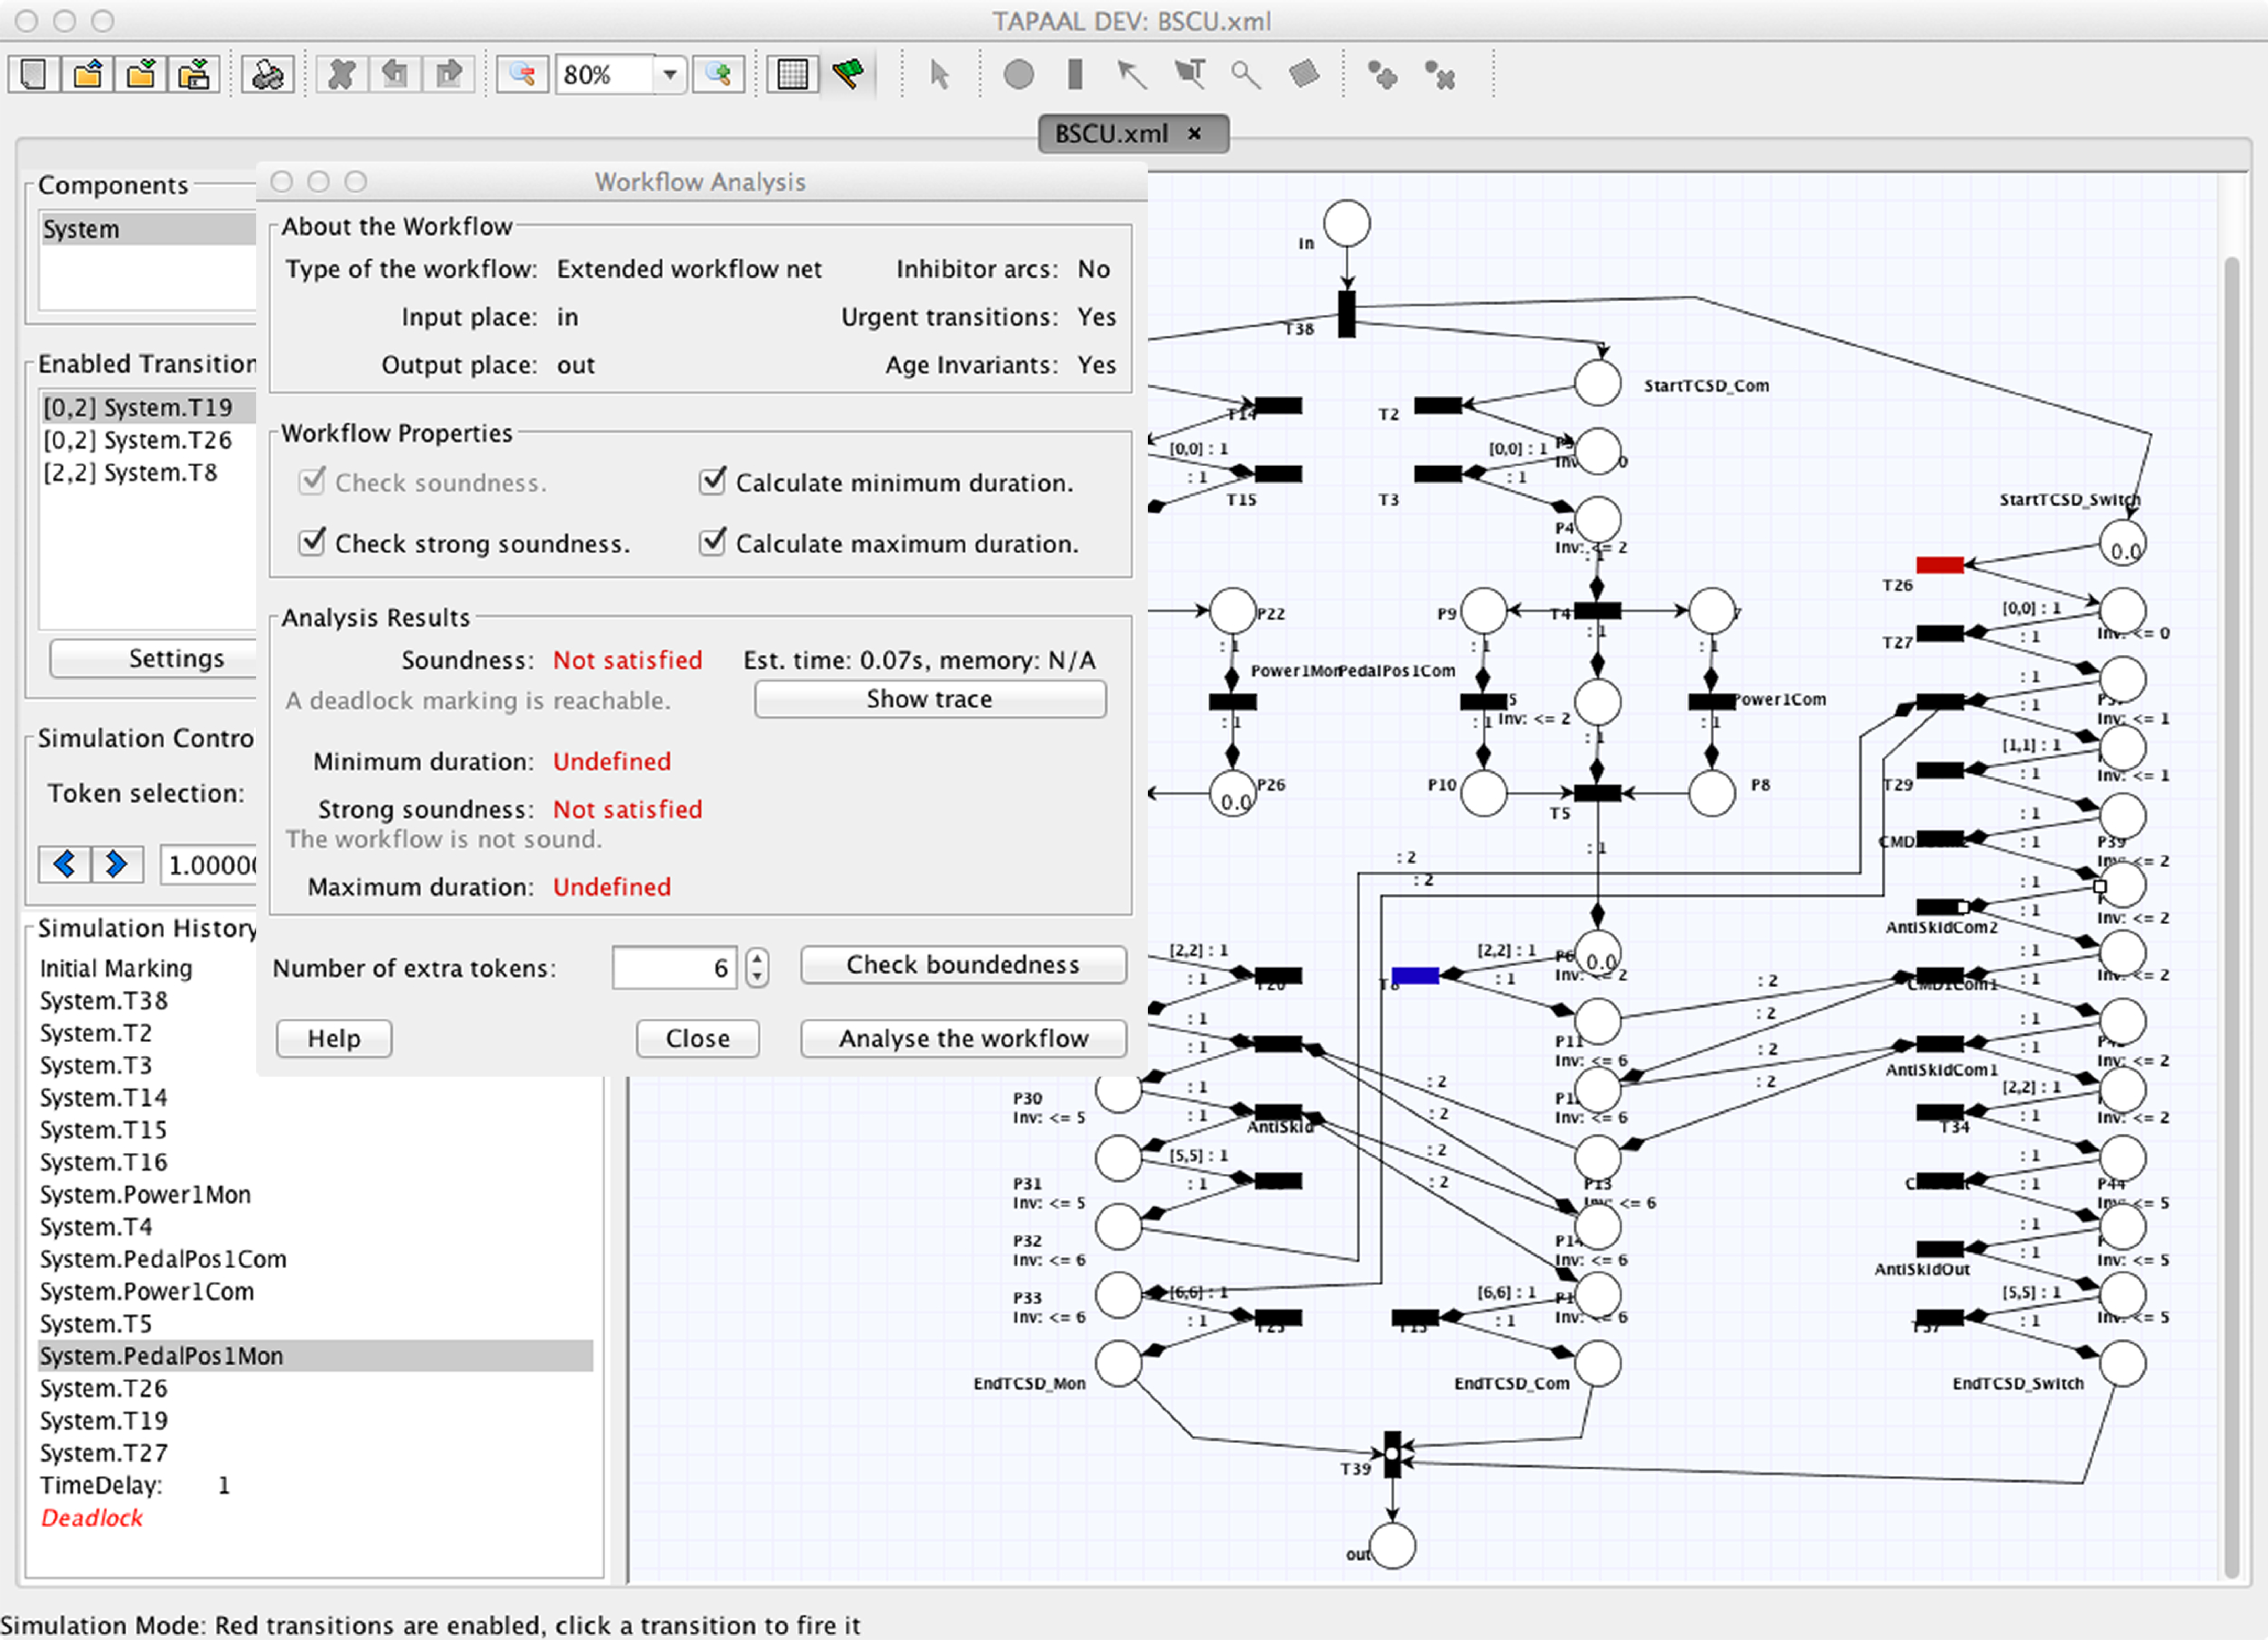
\includegraphics[width=1\textwidth]{Figures/screenshot-combined.eps}
\end{center}
\caption{Screenshot of the workflow analysis tool}
\label{fig:screenshot}
\end{figure}

%\begin{figure}[t]
%\begin{center}
%\includegraphics[height=0.34\textheight]{screenshot1.pdf}
%\includegraphics[height=0.34\textheight]{screenshot2.pdf}
%\end{center}
%\vspace{-4mm}
%\caption{Screenshots of the workflow analysis tool}
%\label{fig:screenshot}
%\end{figure}

We demonstrate the usability of our framework on three case studies.
The studied workflows were modelled and verified with the help of 
a publicly available\footnote{Workflow extension is currently available 
as a beta-release at the bottom of the download section at www.tapaal.net.},
open-source tool TAPAAL~\cite{DJJJMS:TACAS:12}, where
the algorithms presented in this paper are efficiently implemented
in C++. The tool provides a convenient GUI support and
one of the main advantages of our tool is the visualization of traces
disproving soundness (see~\cite{FF:AWPN:06} for more discussion on 
this topic).

In the Brake System Control Unit (BSCU) case study, a part of a 
Wheel Braking System (WBS) used for the certification of civil aircrafts 
in the SAE standard ARP4761~\cite{SEB:FESCA:13}, we discovered  
in less than 1 second that the workflow is not sound due to 
unexpected deadlocks. The authors of~\cite{SEB:FESCA:13} 
were able to detect these problems asking a reachability query,
however, the error traces contradicting soundness were constructed
manually. Our implementation allows a fully automatic detection and
visualization of such situations.

In the second case study describing the workflow of MPEG2 encoding algorithm
run on a multicore processor (Petri net model was taken 
from~\cite{PCVMP:MMM:04}), we verified in about 10 seconds 
both soundness and strong soundness, and computed 
the minimum and maximum encoding time for the IBBP frame sequence.

In the third case study, we checked the soundness 
of a larger blood transfusion workflow~\cite{blood-benchmark},
the benchmarking case study of the little-JIL language. 
The Petri net model was suggested in~\cite{BLS:FHIES:12} but we discovered 
several issues with improper workflow termination that were fixed
and then both soundness and strong soundness was confirmed
in about 1 second, including the information about the minimum 
and maximum execution times. 

TAPAAL models of all case studies can be obtained from www.tapaal.net
and Figure~\ref{fig:screenshot} shows a screenshot of the GUI in the
trace debugging mode for workflow analysis of the brake system control 
unit mentioned above.

\section{Summary}\label{sumWorkflow}
\markright{~\ref{sumWorkflow} Summary}

We presented a framework for modelling of timed workflow processes
via timed-arc workflow nets and studied the classical problem of
soundness and its extension to time-bounded (strong) soundness.
We provided a comprehensive analysis of decidability/undecidability
of soundness and strong soundness on different subclasses of timed-arc
workflow nets. We also suggested efficient algorithms for computing
minimum and maximum execution times of a given workflow and implemented
all algorithms within the tool TAPAAL~\cite{DJJJMS:TACAS:12}. 
As a result we have a complete theory for checking soundness on
timed workflow nets and contrary to many other papers studying
different variants of workflow processes, we took a step further
by providing efficient implementation of the algorithms, including
a platform independent GUI support for modular design of timed
workflow nets and visual error trace debugging. The tool is open-source
and freely available at \url{www.tapaal.net}.
The practical usability of 
the approach was documented on three industry-inspired case studies,
demonstrating a very promising potential for verification of larger
timed workflows.

In the study we focused on the discrete semantics 
of workflow nets that is often sufficient and allows for modelling
of workflows where events can happen in discrete steps.
Nevertheless, we argued that many of the results
are valid also for the continuous semantics. In fact, once we
know that a given net is sound in the continuous semantics,
it is enough to check for strong soundness and minimum/maximum
execution times in the discrete semantics and these answers
are valid also for the continuous case. As a future work, we 
are developing efficient algorithms to decide soundness 
of bounded timed-arc workflow nets in the continuous semantics.
\cleardoublepage

\chapter{Conclusions, Contributions and Future Works}\label{chapter:c6}
\markboth{Chapter~\ref{c6} Conclusions, Contributions and Future Works}{}

This chapter presents the conclusions of this Thesis, reviews the contributions of this work, and suggests some possible future lines of research. It also includes a list of the publications obtained as a result of this work.

%\section{Conclusions}\label{conclusions}
%\markright{~\ref{conclusions} Conclusions}
%
%The work that has been carried out in this Thesis can be divided in two different topics: on the one hand the design and verification of Web Service compositions with time constraints by means of a top-down methodology called Correct-WS and the implementation of the WST tool supporting several phases of this methodology, and on the other hand the specification, validation and verification of electronic contracts with time constraints by means of the definition of a visual model with a formal background called \codiag.
%
%Concerning the first topic, the work carried out in \cite{Cambronero2007} has been continued and extended, adding things such as the treatment of exceptions. The WST tool has been improved in several aspects, completing the implementation of the translation from WS-CDL to timed automata and including the treatment of exceptions in all the different phases supported by the tool.
%
%The advantage of having the Correct-WS methodology and the WST tool is that the correctness of the Web Service compositions, with respect to some properties of interest, can be formally verified in the early phases of the development process. In this way, any problem detected can be solved before implementation, saving the cost of correcting these errors after implementation.
%Another important advantage is that we can obtain automatically XML code from a graphical model of the composition, so non-XML experts do not have to care about specifying the composition in languages such as WS-CDL.
%
%Regarding the second topic, a novel approach for the specification and verification of deontic e-contracts has been defined. It consists of a visual model called \codiag\ representing the obligations, permissions and prohibitions of the contract, including also any condition, reparation and time constraint. The syntax of the model has been formally defined, and the semantics is provided by means of a transformation into a network of timed automata, allowing the verification of some properties of interest on it by using the model-checker of the UPPAAL tool.
%
%Apart from the timed automata semantics, some other applications of \codiag\ are envisaged. They can be used as a user-friendly way of specifying a contract in \CL\ language, as a translation function from \codiag\ to \CL\ has been defined. The diagrams can also be used to check if the behaviours of systems, modelled as timed automata, comply with the contracts represented by \codiag. This can be done by applying the set of satisfaction rules that has been defined.
%
%The main advantage of \codiag\ is that they provide a graphical representation of e-contracts but amenable to formal verification. In this way, non-experts in formal methods can easily specify the contracts in a graphical manner and, as a formal semantics of the model has been defined, the specified contract can be formally verified with respect to some properties of interest. The formal verification of the e-contracts is important to find out any contradiction or unexpected behaviours allowed by the contract, so the contracts can be corrected in a suitable manner.
%
%\section{Contributions}\label{contributions}
%\markright{~\ref{contributions} Contributions}
%
%In this section the contributions produced as a result of the development of this Thesis are summarized in the following list:
%
%\begin{itemize}
%
%\item The continuation and extension of the development of the Correct-WS methodology for the design and verification of Web Service compositions.
%
%\item The improvement of the implementation of the WST tool that supports several phases of the Correct-WS methodology.
%
%\item The definition of a visual model called \codiag\ for the specification of deontic electronic contracts including time constraints.
%
%\item The definition of formal syntax and semantics for \codiag, allowing the formal verification of the contract modelled.
%
%\item The definition of a set of satisfaction rules to check the compliance of the contracts represented by \codiag.
%
%\item The definition of a translation function from \codiag\ to the contract language \CL.
%
%\end{itemize}
%
%\section{Future Works}\label{future}
%\markright{~\ref{future} Future Works}
%
%The work that has been presented in this Thesis has led to several ideas for future work. Some of them are the following:
%
%\begin{itemize}
%
%\item Concerning the WST tool, it is currently under development a new tab supporting the analysis phase of the Correct-WS methodology. This tab will allow the users to develop the KAOS model for the specification of the properties of interest, generating automatically the queries corresponding to this model that have to be check in the verifier of the UPPAAL tool. The inclusion of the translation of WS-CDL documents into Coloured Petri nets in the WST tool is also under development.
%
%\item A study of the complexity and scalability of \codiag\ to see how complex can be the electronic contracts that we can tackle with these diagrams.
%
%\item The application of \codiag\ to different contexts, such as requirements engineering (to formalize
%requirements), product software families (as an extension of feature diagrams), \ldots
%
%\item The development of a tool to model \codiag\ and automatizing the transformation of the diagrams into timed automata supported by the UPPAAL tool, in the same way that the WST tool automatizes several transformations of the Correct-WS methodology.
%
%\item The development of a query language for contracts making possible the specification at a high level of abstraction of the properties of the contracts we want to check, instead of specifying the properties directly in the query language used by the UPPAAL tool. Therefore, a correspondence between the contract query language and the UPPAAL query language would be necessary.
%
%\item We also envisage the possibility of specifying a different diagram for each one of the parties involved instead of having global \codiag\ with multiple agents. This compositional approach can be useful if a composition operator is defined, specifying when two of these new \codiag\ can be composed and the result of the composition.
%
%\end{itemize}
%
%\section{Publications and Collaborations}\label{publications}
%\markright{~\ref{publications} Publications}
%
%The work done during this Thesis has given rise to several publications. They include international journal papers, international conference papers, and a national conference paper. Two technical reports have also been published and works submitted for publication are mentioned too.
%
%\subsection{Journal Papers}
%
%\begin{itemize}
%
%\item 
%Cambronero, M.E., D\'iaz, G., Mart\'inez, E., Valero, V. and Tobarra, L. (2010).
%WST: A Tool Supporting Timed Composite Web Services Model Transformation, \emph{SIMULATION: Transactions of the Society for Modeling and Simulation International}.
%
%\item 
%Cambronero, M.E., D\'iaz, G., Valero, V. and Mart\'inez, E. (2011).
%Validation and Verification of Web Services Choreographies by Using Timed Automata, \emph{Journal of Logic and Algebraic Programming} \textbf{80} pp. 25-49.
%
%\item 
%Cambronero, M.E., Valero, V. and Mart\'inez, E.
%Design and Generation of Web Services Choreographies with Time Constraints, \emph{Journal of Universal Computer Science}, to appear in 2011.
%
%\end{itemize}
%
%\subsection{International Conference Papers}
%
%\begin{itemize}
%
%\item
%Cambronero, M.E., D\'iaz, G., Valero, V. and Mart\'inez, E. (2008). A Tool for the Design and Verification of Composite Web Services, in \emph{Second International Workshop on Formal Languages and Analysis of Contract-Oriented Software}, pp. 9-16.
%
%\item 
%Mart\'inez, E., D\'iaz, G., Cambronero, M.E. and Valero, V. (2009). Design and Verification of Web Services Compositions, in \emph{The Fourth International Conference on Internet and Web Applications and Services}, pp. 395-400.
%
%\item
%Valero, V., Macia, H. and Mart\'inez, E.(2009). Transforming WS-CDL specifications into Coloured Petri Nets, in \emph{International Workshop on Petri Nets and Software Engineering (PNSE09)}.
%
%\item
%Mart\'inez, E., D\'iaz, G., Mart\'inez, C.R., Cambronero, M.E. and Valero, V. (2009). Time Ordering Architecture in SCA, in \emph{TAMoCo 2009 Techniques and Applications for Mobile Commerce}, pp. 117-125.
%
%\item
%Cambronero, M.E., D\'iaz, G., Mart\'inez, E. and Valero, V. (2009). A comparative study between WSCI, WS-CDL, and OWL-S, in \emph{The 2009 IEEE International Conference on e-Business Engineering (ICEBE 2009)}, pp. 377-382.
%
%\item 
%Andr\'es, C., D\'iaz, G., Mart\'inez, E. and Zhang, Y (2009). Formal Study of Prioritized Service Compositions, in \emph{International conference on signal-image technology \& internet based systems, 5th (SITIS 2009)}, pp. 355-362.
%
%\item 
%Mateo, J.A., D\'iaz, G., Mart\'inez, E. and Cambronero, M.E. (2010). Modeling Conference Contribution Management Using Web Services, in \emph{The Fifth International Conference on Internet and Web Applications and Services}, pp. 463-468.
%
%\item
%Mart\'inez, E., D\'iaz, G., Cambronero, M.E. and Schneider, G. (2010). A Model for Visual Specification of e-Contracts, in \emph{The 7th IEEE International Conference on Services Computing (SCC 2010)}, pp. 1-8.
%
%\item
%Mart\'inez, E. and Schneider, G. (2010). Automated Analysis of Conflicts in Software Product Lines, in \emph{1st International Workshop on Formal Methods in Software Product Lines Engineering}, pp. 75-82.
%
%\item
%Mart\'inez, E., D\'iaz G. and Cambronero, M.E. (2010). Visual Specification of Formal e-Contracts, in \emph{Fourth Workshop on Formal Languages and Analysis of Contract-Oriented Software}, pp. 55-62.
%
%\item
%Mateo, J.A., Valero, V., Mart\'inez, E. and D\'iaz, G. (2011). Analysis and Verification of Web Services Resource Framework (WSRF) specifications Using Timed Automata Modeling Conference Contribution Management Using Web Services, in \emph{The Sixth International Conference on Internet and Web Applications and Services}, pp. 222-227.
%
%\item
%Mart\'inez, E., Cambronero, M.E., D\'iaz, G. and Schneider, G. (2011). Timed Automata Semantics for Visual e-Contracts, in \emph{Fifth Workshop on Formal Languages and Analysis of Contract-Oriented Software}, pp. 7-22.
%
%\item
%Mart\'inez, E., D\'iaz, G. and Cambronero, M.E. Contractually Compliant Service Compositions, \emph{The Ninth International Conference on Service Oriented Computing}, to appear in 2011.
%
%\end{itemize}
%
%\subsection{National Conference Papers}
%
%\begin{itemize}
%
%\item 
%Valero, V., Macia, H. and Mart\'inez, E.(2009). A Petri Net Semantics for WS-CDL, in \emph{XVII Jornadas de Concurrencia y Sistemas Distribuidos}, pp. 35-50.
%
%\end{itemize}
%
%\subsection{Technical Reports}
%
%\begin{itemize}
%
%\item Cambronero, M.E., Valero, V., D\'iaz, G. and Mart\'inez, E. (2009). Web Services Choreographies Verification, \emph{Technical Report DIAB-09-04-3}, Computing Systems Department, University of Castilla-La Mancha.
%
%\item Cambronero, M.E., D\'iaz, G., Mart\'inez, E. and Valero, V. (2009). A comparative study between WSCI, WS-CDL, and OWL-S, \emph{Technical Report DIAB-09-04-3}, Computing Systems Department, University of Castilla-La Mancha.
%
%\end{itemize}
%
%%\subsection{Submitted Works}
%
%\subsection{Collaborations}
%
%International Collaborations and stays at international universities and research groups:
%
%\begin{itemize}
%
%\item Department of Applied IT at Chalmers | University of Gothenburg - Sweden for 3 months in 2009.
%
%\end{itemize}
%
%\section{Funds and Grants}\label{funds}
%\markright{~\ref{funds} Funds and Grants}
%
%The present Thesis has been carried out thanks to the funds received from a number of projects and grants:
%
%\begin{itemize}
%
%\item Research project: Modelling and Analysis of Composed Web Services Using Formal Techniques (TIN2009-14312-C02-02)\newline
%Research project funded by Spanish Ministry of Education \& Science.\newline
%Participating Organizations: University de Castilla-La Mancha (Spain).
%
%\item The author of this thesis has been supported by a predoctoral grant from the \textit{Junta de Comunidades de Castilla-La Mancha}, as a part of the program ``\textit{Plan Regional de Investigaci\'{o}n Cient\'{\i}fica, Desarrollo Tecnol\'{o}gico e Innovaci\'{o}n 2005-2010 (PRINCET)}''.
%
%\end{itemize}
\cleardoublepage

\appendix

%\chapter{XSL, XPath, and XSLT}\label{a1}
\markboth{Appendix~\ref{a1}. XSL, XPath, and XSLT}{}

\section{Extensible Stylesheet Language (XSL)}\label{XSL}
\markright{~\ref{XSL} Extensible Stylesheet Language (XSL)}

\begin{figure}[h]
\begin{center}
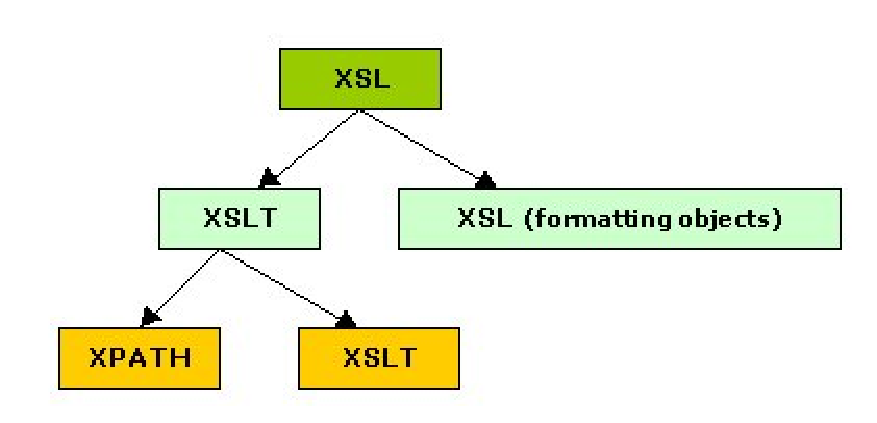
\psfig{file=Figures/esquema.eps,scale=.75}
\end{center}
\caption{Schema of the relationship between XSL, XPath, and XSLT.}
\label{FigureA1}
\end{figure}

The Extensible Stylesheet Language (XSL) \cite{W3C2006} is a language developed by the W3C based on XML that is used to specify how the information in an XML document is transformed to create a new document. This new document can be another XML document, an HTML we want to display in a browser, \ldots\ XSL language was formerly divided into two parts: (i) a transformation language specifying how the transformation between documents is done, and (ii) a formatting language specifying how the resulting XML documents will be.

During the development of the XSL standard the transformation language was split into a different specification called Extensible Stylesheet Language Transformations (XSLT). Moreover, the part of the XSLT language responsible for accessing and navigating the nodes of the XML document was also split into another language. This language was called XML Path Language (XPath) and is intended to be used together with XSLT.

In Figure \ref{FigureA1} we can see a schema showing the relationship between these three specification languages.

\section{XML Path Language (XPath)}\label{XPath}
\markright{~\ref{XPath} XML Path Language (XPath)}

XML Path Language (XPath) \cite{W3C1999} is a language used to find information inside an XML document. The language allows us to navigate across the different elements and attributes composing the document.

XPath uses \textbf{path expressions} to do the nodes selection inside the XML document. These expressions are very similar to the paths used by file systems in operating systems like Windows or Linux.

XPath also provides more than 100 \textbf{functions} offering capabilities such as manipulation of strings, manipulation of numerical values, data comparisons, \ldots

In XPath we can distinguish seven different types of node: root nodes, element nodes, text nodes, attribute nodes, namespace nodes, processing instruction nodes and comment nodes. An XML document is treated as a tree of these nodes, where we have the following relationships between the nodes:

\begin{itemize}

\item \textbf{Parent}: Each element in the document has a parent except the root node.

\item \textbf{Children}: Each element can have zero, one or more children.

\item \textbf{Siblings}: Elements with the same parent are considered siblings.

\item \textbf{Ancestor}: We consider ancestors of an element its parent, its parent's parent, \ldots

\item \textbf{Descendant}: We consider descendants of an element its children, its children's children, \ldots

\end{itemize}

The selection of nodes in XPath is done by following a path. Some of the most common path expressions are the following, where several of them can be combined by means of the operator \textbf{$|$}:

\begin{itemize}

\item \textbf{nodename}: It selects all the children with name \textit{nodename}.

\item \textbf{/}: It selects from the root node.

\item \textbf{//}: It selects the nodes in the document satisfying the selection condition given next, without taking into account the place in the hierarchy where they are.

\item \textbf{.}: It selects the current node.

\item \textbf{..}: It selects the parent of the current node.

\item \textbf{@}: It selects attributes of the node.

\end{itemize}

Predicates are used in XPath to find a node having an specific name or containing an specific value. These predicates are always written inside square brackets (\textit{[]}) and some of the most common are the following, where the symbol \textbf{*} can be used as a wildcard:

\begin{itemize}

\item \textbf{nodename[1]}: It selects the first child of the current node with name \textit{nodename}.

\item \textbf{nodename[last()]}: It selects the last child of the current node with name \textit{nodename}.

\item \textbf{nodename[position $<$ 3]}: It selects the first two children of the current node with name \textit{nodename}.

\item \textbf{nodename[@lang]}: It selects the children of the current node with name \textit{nodename} and having an attribute \textit{lang}.

\item \textbf{nodename[@lang=``es'']}: It selects the children of the current node with name \textit{nodename} and having an attribute \textit{lang} with value \textit{``es''}.

\item \textbf{nodename[price $>$ 20]}: It selects the children of the current node with name \textit{nodename} and having a child element named \textit{price} with a value over \textit{20}.

\end{itemize}

Axes are used in XPath to define a set of nodes relative to the current node. The axes defined in the language are the following:

\begin{itemize}

\item \textbf{ancestor}: It selects all the ancestor nodes of the current node.

\item \textbf{ancestor-or-self}: It selects all the ancestor nodes of the current node and the current node itself.

\item \textbf{attribute}: It selects all the attributes of the current node.

\item \textbf{child}: It selects all the children of the current node.

\item \textbf{descendant}: It selects all the descendants of the current node.

\item \textbf{descendant-or-self}: It selects all the descendants of the current node and the current node itself.

\item \textbf{following}: It selects all the elements in the document after the closing label of the current node.

\item \textbf{following-sibling}: It selects all the subsequent siblings of the current node.

\item \textbf{namespace}: It selects all the namespace nodes inside the current node.

\item \textbf{parent}: It selects the parent of the current node.

\item \textbf{preceding}: It selects all the elements in the document before the opening label of the current node.

\item \textbf{preceding-sibling}: It selects all the previous siblings of the current node.

\item \textbf{self}: It selects the current node.

\end{itemize}

There are also a set of operators that can be used in XPath expressions. They are the following:

\begin{itemize}

\item \textbf{$|$}: It is used to combine two sets of nodes.

\item \textbf{+}: Addition.

\item \textbf{-}: subtraction;.

\item \textbf{*}: Multiplication.

\item \textbf{div}: Division.

\item \textbf{=}: Equality.

\item \textbf{!=}: Inequality.

\item \textbf{$<$}: Less than.

\item \textbf{$<$=}: Less or equal than.

\item \textbf{$>$}: Greater than.

\item \textbf{$>$=}: Greater or equal than.

\item \textbf{or}: Logic operator ``or''.

\item \textbf{and}: Logic operator ``and''.

\item \textbf{mod}: Modulus operator.

\end{itemize}

Finally, XPath also provides a library of functions for multiple purposes: error functions, numeric functions, string manipulation functions, date functions,\ldots

\section{Extensible Stylesheet Language Transformations (XSLT)}\label{XSLT}
\markright{~\ref{XSLT} Extensible Stylesheet Language Transformations (XSLT)}

Extensible Stylesheet Language Transformations (XSLT) \cite{W3C1999-2} is the most important part of XSL. By using XSLT we can add or delete elements and attributes in the generated output document. It also allows us to order elements, make queries and make decisions about which elements are included and which elements are not included in the output document

In the process of transformation, XSLT uses XPath to define parts of the input document that must correspond with one or several templates. If one of these parts is found in the input document, XSLT does the transformation of it into the output document.

The root element of an XSLT document is always $<$xsl:stylesheet$>$ or $<$xsl:transform$>$.

The element $<$xsl:template$>$ is used to build templates. The attribute \textit{match} is used to match a template with an XML element. To define a template corresponding to the full XML document, this attribute must have the value \textbf{/}.

The element $<$xsl:value-of$>$ is used to extract a value from the input XML and adding it to the output XML, using the attribute \textit{select} for this purpose.

The element $<$xsl:sort$>$ is used to order the output by including this element inside element $<$xsl:for-each$>$ and 
using the attribute \textit{select} to specify the ordination criteria.

The element $<$xsl:if$>$ is used to evaluate a condition and its internal code is only executed if this condition is fulfilled, otherwise its code would have no effect. The attribute \textit{test} is used to specify the condition.

The element $<$xsl:choose$>$ is used together with the elements $<$xsl:when$>$ and $<$xsl:otherwise$>$ to evaluate multiple conditions.

The element $<$xsl:apply-templates$>$ applies a template over the current node or over the children of the current node. If the attribute \textit{select} is included only the children corresponding to the attribute value will be processed. In this way, the attribute can be used to determine the order in which children are processed.

There are still more elements that can be used in XSLT: the element \textit{text} to directly write any text in the output document, the element \textit{element} to create the specified node in the output document, the element \textit{call-template} to call templates by means of their name, \ldots
\bibliographystyle{plain}
\bibliography{Bibliography,bibliography}

%%%%%%%%%%%%%%%%%%%%%%%%%%%%%%%%%%%%%%%%%%%%%%%%%%%%%%%%%%%%%%%%%%%%%%%%%%%%%%%%%%%%%%%%%%%%%%
\markboth{\bibname}{\bibname}

\addcontentsline{toc}{chapter}{\bibname}

\bibliography{bibliography}

\cleardoublepage

\end{document}
